\documentclass[final]{ruthesis}
\special{papersize=8.5in,11in} %***for A4-default configurations on servers
\phd

\documentclass[10pts]{article}

%% Language and font encodings
\usepackage[english]{babel}
\usepackage[utf8x]{inputenc}
\usepackage[T1]{fontenc}
\usepackage{float}
\usepackage{listings}
\usepackage{nicefrac}
%% Sets page size and margins
\usepackage[letterpaper,top=3cm,bottom=2cm,left=3cm,right=3cm,marginparwidth=1.75cm]{geometry}

%% Useful packages
\usepackage{amsmath}
\usepackage{amsthm}
\usepackage{graphicx}
\usepackage{subcaption}
\usepackage{color}
\usepackage{xcolor}
\usepackage[colorlinks,allcolors=blue]{hyperref}
\usepackage{cleveref}
\usepackage{booktabs}
\usepackage{multirow}
\usepackage{paralist}
\usepackage{cite}
%\definecolor{codegreen}{rgb}{0,0.6,0}
%\definecolor{codegray}{rgb}{0.5,0.5,0.5}
%\definecolor{codepurple}{rgb}{0.58,0,0.82}
%\definecolor{backcolour}{rgb}{0.95,0.95,0.92}

\newif\ifdraft
\drafttrue
\ifdraft
\definecolor{ocolor}{rgb}{1,0,0.4}
\newcommand{\jwave}[1]{ {\reduwave{#1}}}
\newcommand{\jhanote}[1]{ {\textcolor{red} { ***shantenu: #1 }}}
\newcommand{\mtnote}[1]{ {\textcolor{cyan} { ***matteo: #1 }}}
\definecolor{orange}{rgb}{1,.5,0}
\definecolor{dandelion}{cmyk}{0,0.29,0.84,0}
\newcommand{\gpnote}[1]{{\textcolor{green} {***giannis: #1}}}
\newcommand{\note}[1]{ {\textcolor{magenta} { ***Note: #1 }}}
\else
\newcommand{\jwave}[1]{}
\newcommand{\jhanote}[1]{}
\newcommand{\mtnote}[1]{}
\newcommand{\gpnote}[1]{}
\newcommand{\note}[1]{}
\fi

\theoremstyle{definition}
\newtheorem{defn}{Definition}[section]

\lstdefinestyle{mystyle}{
    backgroundcolor=\color{backcolour},   
    commentstyle=\color{codegreen},
    keywordstyle=\color{magenta},
    numberstyle=\tiny\color{codegray},
    stringstyle=\color{codepurple},
    basicstyle=\footnotesize,
    breakatwhitespace=false,         
    breaklines=true,                 
    captionpos=b,                    
    keepspaces=true,                 
    numbers=left,                    
    numbersep=5pt,                  
    showspaces=false,                
    showstringspaces=false,
    showtabs=false,                  
    tabsize=2
}
 
\lstset{style=mystyle}
\setcounter{tocdepth}{3}

\begin{document}

\author{Ioannis Paraskevakos}
\copyrightp
\title{Software Systems for Supporting Scientific Campaigns on High Performance \& Distributed Computing Resources}
\author{Ioannis Paraskevakos}
\program{Electrical and Computer Engineering}
\director{Dr. Shantenu Jha and Dr. Matteo Turilli}
\approvals{4}
\submissionyear{2020}
\submissionmonth{October}
\figurespage
\tablespage

\abstract{% !TEX root = main.tex
Computational sciences such as biomolecular sciences~\cite{cheatham2015impact,
dakka2018concurrent}, ecological sciences~\cite{goncalves2020sealnet,
paraskevakos2019workflow} and particle physics~\cite{atlas} execute multiple
workflows to achieve scientific insight. Users submit multiple workflows for
execution and monitor their execution while achieving a computational objective.
This way of execution multiple workflows is called a computational campaign.

This dissertation addresses the problem of effectively and efficiently executing
a computational campaign on High Performance Computing (HPC) resources.
Specifically, the dissertation focuses on computational campaigns with
data-intensive workflows that utilize HPC resources at scale.

Data-intensive workflows are not well supported on HPC resources. However, the
MapReduce abstraction is used successfully to execute at scale data-intensive
workflows on cloud resources. Utilizing the MapReduce abstraction on HPC
resources has the potential to efficiently execute data-intensive workflows on
HPC resources. Thus, we utilize the Pilot-Abstraction as an integrating concept
between HPC and MapReduce frameworks (e.g., Hadoop) by extending RADICAL-Pilot,
a Pilot-Abstraction framework, to support Hadoop on HPC resources. We then
experimentally characterize the execution time of data-intensive workflows and
extension's overheads and show that Hadoop indeed reduces the execution time of
such workflows on HPC resources.

However, MapReduce frameworks offer different abstraction and capabilities and
no single framework suits any type of data-intensive workflow, as they have
different characteristics (e.g., MapReduce or embarrassingly parallel). As
MapReduce frameworks utilize task-parallelism to execute workflows in a
scalable and efficient manner, we experimentally investigate the suitability of
three task-parallel frameworks for the execution of data-intensive workflows on
HPC resources. Based on our experimental analysis, we provide a conceptual
model as to which framework is more suitable based on the characteristics of
the data-intensive workflows. The conceptual model along with the extension of
the Pilot-Abstraction provide a methodology for application developers to
maximize resource utilization while reducing the engineering effort needed to
develop and execute data analysis workflows on HPC resources.

In addition to MapReduce style workflows, there are data-intensive workflows
that do not necessarily conform to MapReduce. These workflows are data-
and compute-intensive requiring efficient utilization of heterogeneous 
resources. Further, there are architecturally equivalent task-parallel designs
to support such workflows. Selecting a suitable design can significantly
increase resource utilization and reduce any overhead imposed by the design. To
that extent, we implement and experimentally characterize three equivalent
designs and show which design approach is best suited for scientific workflows
with similar characteristics.

After establishing the methodology to effectively and efficiently execute
data-intensive workflows on HPC, we investigate the support of computational
campaigns. We elicit the requirements for a campaign manager from three
scientific computational campaigns. Based on those requirements, we design and
implement a campaign manager prototype. The prototype is domain-agnostic and
adheres to the building blocks design approach. The campaign manager prototype
creates an execution plan and simulates the execution of a campaign on HPC
resources. Further, we investigate three algorithms to derive an execution plan
and characterize their performance in terms of makespan and plan sensitivity to
resource performance changes and workflow runtime estimation uncertainty. Based
on our analysis, we provide a conceptual model for selecting a suitable
planning algorithm based on characteristics of a computational campaign and
resources.

The research of this dissertation makes the following contributions:
\begin{inparaenum}
    \item Integrate MapReduce frameworks and HPC to offer unified environment
    for compute- and data-intensive workflows.
    \item Provide a conceptual model for selecting a task-parallel framework
    based on the workflow requirements and framework abstractions and
    performance
    \item Provide design guidelines for supporting data- and compute-intensive
    workflows on HPC and an experimental methodology to compare equivalent
    designs
    \item Design and implement a campaign manager prototype to plan and execute
    computational campaigns
    \item Provide a conceptual model for selecting a planning algorithm to 
    derive an execution plan based on campaign, resources and algorithm
    characteristics

\end{inparaenum}
}
\acknowledgements{hello}

\beforepreface
\afterpreface

% ---------------------------------------------------------
% CHAPTER 1
% ---------------------------------------------------------
\chapter{Introduction}
\label{ch:intro}
\label{ch:intro}
This is the introduction of my dissertation. This document will try to show all the details of my work over the last six years.

\begin{figure}
    \centering
    \includegraphics{}
    \caption{Caption}
    \label{fig:my_label}
\end{figure}

% ---------------------------------------------------------
% CHAPTER 2
% ---------------------------------------------------------
\chapter{Data Analytics and High Performance Computing}
\label{ch:pilot-data-hadoop}
% !TEX root = main.tex
\label{ch:pilot-data-hadoop}

Computational campaigns on High Performance Computing (HPC) resources can execute compute- or data- intensive workflows and applications.
Compute-intensive applications and workflows are associated with either a single long running executable or an ensemble of compute-intensive tasks~\cite{balasubramanian2018harnessing}.
On the other hand, data-intensive applications are associated with multiple stages of execution which can I/O, memory and compute bound.
While MPI is the most common programming model for compute-intensive applications, the MapReduce~\cite{dean2004mapreduce} abstraction is commonly used for data-intensive applications~\cite{hellerstein2012science}.

%However, HPC resources are designed to support mainly compute-intensive long-running MPI applications, as they offer
%Not surprisingly, HPC resource architectures offer large number of computing resources, e.g., CPUs and GPUs, connected by high-end networks (e.\,g.\ Infiniband) and filesystems, such as Lustre and PVFS.
%They have however limitations in supporting data-intensive and I/O bound workflows.

Hadoop~\cite{hadoop} popularized the use of MapReduce~\cite{dean2004mapreduce} for data-intensive applications.
Hadoop's distirbuted filesystem (HDFS) automatically partitions data and distributes them to different nodes in a distributed cluster.
In addition, Hadoop's engine takes advantage of data-locality and transfers computations to nodes allowing to process data in parallel while reducing data transfers.
While Hadoop simplified the processing of vast volumes of data, it has limitations in its expressiveness~\cite{yelick2011magellan,isard2007dryad}.
The complexity of creating sophisticated applications such as iterative machine learning algorithms required multiple MapReduce jobs and persistence to Hadoop's Filesystem (HDFS) after each iteration.
This lead to several higher-level abstractions for implementing sophisticated data pipelines.

The most well-known processing framework in the Hadoop ecosystem is Spark~\cite{zaharia2010spark}.
In contrast to MapReduce, it provides a richer API, more language bindings and a memory-centric processing engine that can utilize distributed memory and retain resources across multiple task generations.
Spark's \emph{Reliable Distributed Dataset (RDD)} ~\cite{zaharia2012resilient} abstraction provides a powerful way to manipulate distributed collections stored in cluster nodes' memory.
Spark is used for building complex data workflows and advanced analytic tools, such as MLLib~\cite{mllib}.
Although the addition/development of new and higher-level execution frameworks addressed some of the problems of data processing, it introduced the problem of heterogeneity of access and resource management.

% Problem statement.
Some computational campaigns cannot be easily classified as only compute- or data-intensive, such as bio-molecular dynamics~\cite{dror2012biomolecular}.
Bio-molecular simulations are now high-performant, reach increasing time scales and problem sizes, and thus generating immense amounts of data.
Often times the data generated needs to be analyzed so as to determine the next set of simulation configurations.
Several tools evolved to meet the demand for molecular dynamics data analysis, such MDAnalysis~\cite{michaud2011mdanalysis,gowers2016mdanalysis}, CPPTraj~\cite{roe2013ptraj} and HiMach~\cite{tiankai2008scalable}.
Although these tools offer domain-specific analytics, scaling them to high data volumes remains a challenge.
This points to the need for environments that support scalable data processing while preserving the ability to run simulations at the scale so as to generate the data.
To the best of our knowledge, there does not exist a solution that provides the integrated capabilities of Hadoop and HPC.

% Solution
In this chapter, we explore the integration between Hadoop~\cite{hadoop}, and Spark~\cite{zaharia2010spark} and HPC resources.
We utilize the Pilot-Abstraction~\cite{luckow2012pstar} allowing to manage HPC and data-intensive applications in a uniform way.
We explore two extensions to RADICAL-Pilot~\cite{merzky2018design}, a Pilot-Job~\cite{luckow2012pstar} runtime system designed for implementing task-parallel applications on HPC: 
\begin{inparaenum}[1)]
    \item the ability to spawn and manage Hadoop/Spark clusters on HPC infrastructures on demand (Mode I); and
    \item to connect and utilize Hadoop and Spark clusters for HPC applications (Mode II)
\end{inparaenum}.
Both extensions facilitate the complex application and resource management requirements of data-intensive applications.
By supporting these two usage modes, RADICAL-Pilot dramatically simplifies the barrier of deploying and executing HPC and Hadoop/Spark workflows side-by-side.

The chapter is organized as follows: In section~\ref{sec:hpc_hadoop_rel} we discuss the current solutions and challenges of integrating data analytics and HPC.
We continue with discussing the modes of integration and interoperability between data analytics and HPC in \S~\ref{sec:integration_mode} and the experimental validations of the integration in ~\S~\ref{sec:rph-exps}.
The chapter closes with our conclusions in section~\ref{sec:hpc_hadoop_concl}.

\section{Related Work and Challenges}
\label{sec:hpc_hadoop_rel}
\subsection{Related Work}
There are several frameworks which explored the usage of Hadoop on HPC resources, e.\,g., Hadoop on Demand~\cite{hod}, JUMMP~\cite{moody2013jummp}, MagPie~\cite{chu2015magpie}, MyHadoop~\cite{krishnan2011myhadoop}, MyCray~\cite{mycray}.
These frameworks provide users with a set of scripts that can spawn and manage a Hadoop cluster on HPC resources.
As soon as Hadoop is started, users can either submit their MapReduce jobs interactively or via a script.

Although these frameworks can spawn and manage Hadoop clusters, they isolate the Hadoop cluster from the HPC environment.
The scripts and capabilities they offer interact directly with the HPC's submission system.
As a result, users cannot execute on the same set of nodes HPC and Hadoop applications.
Further, they do not necessarily optimize configurations and resource usage, including the use of available SSDs, parallel filesystems and high-end network features, e.\,g.\ RDMA~\cite{rahman2014homr}.

\subsection{Challenges}
Hadoop originally provided a rudimentary resource management system, the YARN scheduler.
The YARN scheduler~\cite{vavilapalli2013apache} provides an application-level scheduling framework addressing the increased requirements with respect to applications and infrastructure, such as more complex data localities (memory, disk, datacenter), long-lived services, periodic jobs, interactive and batch jobs.
In contrast, to batch schedulers of HPC resources, YARN is optimized for supporting data-intensive environments and managing a large number of fine-grained tasks.

While YARN manages system-level resources, applications need to implement an application-level scheduler that optimizes their specific requirements, e.,g., with respect to data locality.
This application-level scheduler, the \textit{Application Master}, is responsible for allocating resources ---called containers---  and executing tasks on these resources.
In addition, the Application Master manages data locality, e.,g., between HDFS blocks and container locations, by allocating containers on specific nodes.

Managing resources on top of YARN is associated with several challenges.
While applications with fine-grained, short-running tasks are well supported, applications with coarse-grained, long-running task, such as MPI applications, are not.
To achieve interoperability and integration between Hadoop and HPC, it is essential to consider a more diverse set of applications on top of YARN.

A particular challenge for Hadoop on HPC deployment is the choice of storage and filesystem backend.
Typically, when using Hadoop local storage is preferred.
Nevertheless, in some cases, e.\,g.\ processing many small files, random data access is required or the number of parallel tasks is low to medium, using a parallel filesystem can yield a better performance.
For this purpose, many parallel filesystems provide a special client library which improves the interoperability with Hadoop, but limits data locality and any data placement optimization.

Another challenge is the integration between both HPC and Hadoop environments.
Rather than preserving HPC and Hadoop ``environments'' as software silos, there is a need for an approach that integrates them. 
We utilize the Pilot-Abstraction as a unifying concept to efficiently support the integration, and not just the interoperability between HPC and Hadoop.
By utilizing the multi-level scheduling capabilities of YARN, the Pilot-Abstraction can efficiently manage Hadoop resources providing an application with the means to reason about data, compute resources and allocation.
In addition, we show how the Pilot-Abstraction can be used to manage Hadoop applications on HPC environments.

The Pilot-Abstraction~\cite{luckow2012pstar} is successfully used on HPC resources supporting a diverse set of task-based workflows.
A Pilot-job is a placeholder job which is submitted to the resource management system and represents a container for a dynamic set of tasks.
Pilot-jobs are, also, a well-known example of multi-level scheduling, which is often used to separate system-level resource and user-level workload management.
The Pilot-Abstraction defines the following entities:
\begin{inparaenum} [1)]
    \item a Pilot which allocates a set of computational resources (e.\,g.\,cores); and
    \item  a Compute-Unit (CU) as a self-contained piece of work represented as an executable.
\end{inparaenum}
The Pilot-Abstraction has been implemented within RADICAL-Pilot~\cite{merzky2018design}.


\section{Data analytics and HPC integration: RADICAL-Pilot and YARN/ Spark}
\label{sec:integration_mode}
Having established the potential of the Pilot~-Abstraction for a range of high-performance applications~\cite{treikalis2016repex,ragothaman2014developing,ko2014numerical}, we use it as the starting point for integrating HPC and data-intensive analytics.
As depicted in Figure~\ref{fig:figures_hadoop-on-hpc-viceverse}, there are at least two different usage modes to consider:
\begin{inparaenum}[1)]
    \item Mode I: Running Hadoop/Spark applications on HPC environments (Hadoop on HPC),
    \item Mode II: Running HPC applications on YARN clusters (HPC on Hadoop).
\end{inparaenum}

\begin{figure}[t]
    \centering
    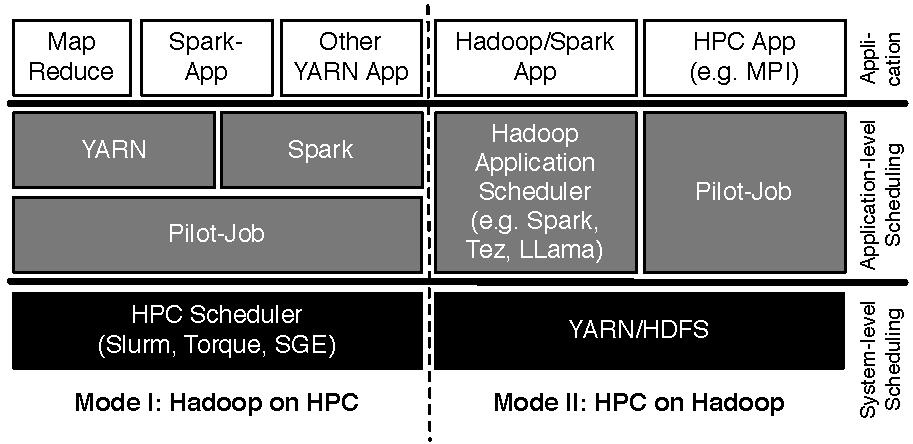
\includegraphics[width=.85\textwidth]{figures/data_analytics_hpc/hpc_hadoop/hadoop-on-hpc-viceverse.pdf}
    \caption{Hadoop and HPC Interoperability modes\label{fig:figures_hadoop-on-hpc-viceverse}}
\end{figure}

Mode I is critical to support traditional HPC environments so as to support applications with both compute and data requirements.
Mode II is important for cloud environments (e.\,g.\ Amazon's Elastic MapReduce) and an emerging class of HPC machines with new architectures and usage modes, such as Wrangler~\cite{wrangler}, that support Hadoop natively.
For example, Wrangler supported dedicated Hadoop environments (based on Cloudera Hadoop 5.3) via a reservation mechanism.
%We discuss, the integration of Hadoop and Spark runtimes into RADICAL-Pilot, which enables both the interoperable use of HPC and Hadoop, as well as the integration of HPC and Hadoop applications (Mode I and II).
Using these new capabilities, applications can seamlessly connect HPC stages (e.\,g.\ simulation stages) with analysis staging using the Pilot-Abstraction to provide unified resource management.
%\subsection{Mode I---II: }
%\label{ssec:rp-impl}

With the introduction of YARN, a broader set of applications can be executed within a Hadoop cluster than earlier.
However, developing and deploying YARN applications potentially side-by-side with HPC applications remains a difficult task.
Established abstractions which are easy to use while enabling users to reason about compute and data resources across infrastructure types (i.\,e.\ Hadoop, HPC and clouds) are missing. 

Schedulers such as YARN effectively facilitate application-level scheduling.
Although, the development efforts for YARN applications are still high.
YARN provides a low-level abstraction for resource management, e.g., a Java API and protocol buffer specification.
Typically interactions between YARN and applications are much more complex than the interactions between an application and an HPC scheduler.
Further, applications must be able to run on a dynamic set of resources; YARN e.\,g.\ can preempt containers in high-load situations.
Data/compute locality need to be manually managed by the application scheduler by requesting resources at the location of a file chunk.
Also, the scheduler can preempt resources (the so called YARN containers).

To address these shortcomings, various frameworks that aid the development of YARN applications have been proposed.
Llama~\cite{llama} offers a long-running application master for YARN designed for the Impala SQL engine.
Apache Slider~\cite{apache-slider} supports long-running distributed application on YARN with dynamic resource needs allowing applications to scale to additional containers on demand.
While these frameworks simplify development, they do not address concerns such as interoperability and integration of HPC/Hadoop.
Integrating YARN and RADICAL-Pilot (RP) allows applications to run HPC and YARN applications on HPC resources concurrently.

\subsubsection*{RADICAL-Pilot and YARN Overview}
\label{sssec:rp_yarn}
% RADICAL-Pilot Overview
Figure~\ref{fig:comp_rp_arch} illustrates the architecture of RADICAL-Pilot and the components that were extended.
The figure on the left shows the macro architecture of RADICAL-Pilot.
The figure on the right shows the architecture of the Pilot-Agent which is a critical functional component.
RADICAL-Pilot consists of a client module with the Pilot-Manager and Unit-Manager and a set of RADICAL-Pilot-Agents running on resources.
The Pilot-Manager is the central entity responsible for managing a set of pilots.
Pilots are described via a Pilot description, which contains the pilot's resource requirements and is submitted to the Pilot-Manager.
The Pilot-Manager, then, submits a placeholder job which will run the RADICAL-Pilot-Agent via the Resource Management System using the SAGA-API~\cite{merzky2015saga} (steps P.1-P.2).
Subsequently, the Unit-Manager and the RADICAL-Pilot-Agent manage the application workload (the Compute-Units,steps U.1-U.7)~\cite{merzky2019using}.

\begin{figure}
    \centering
    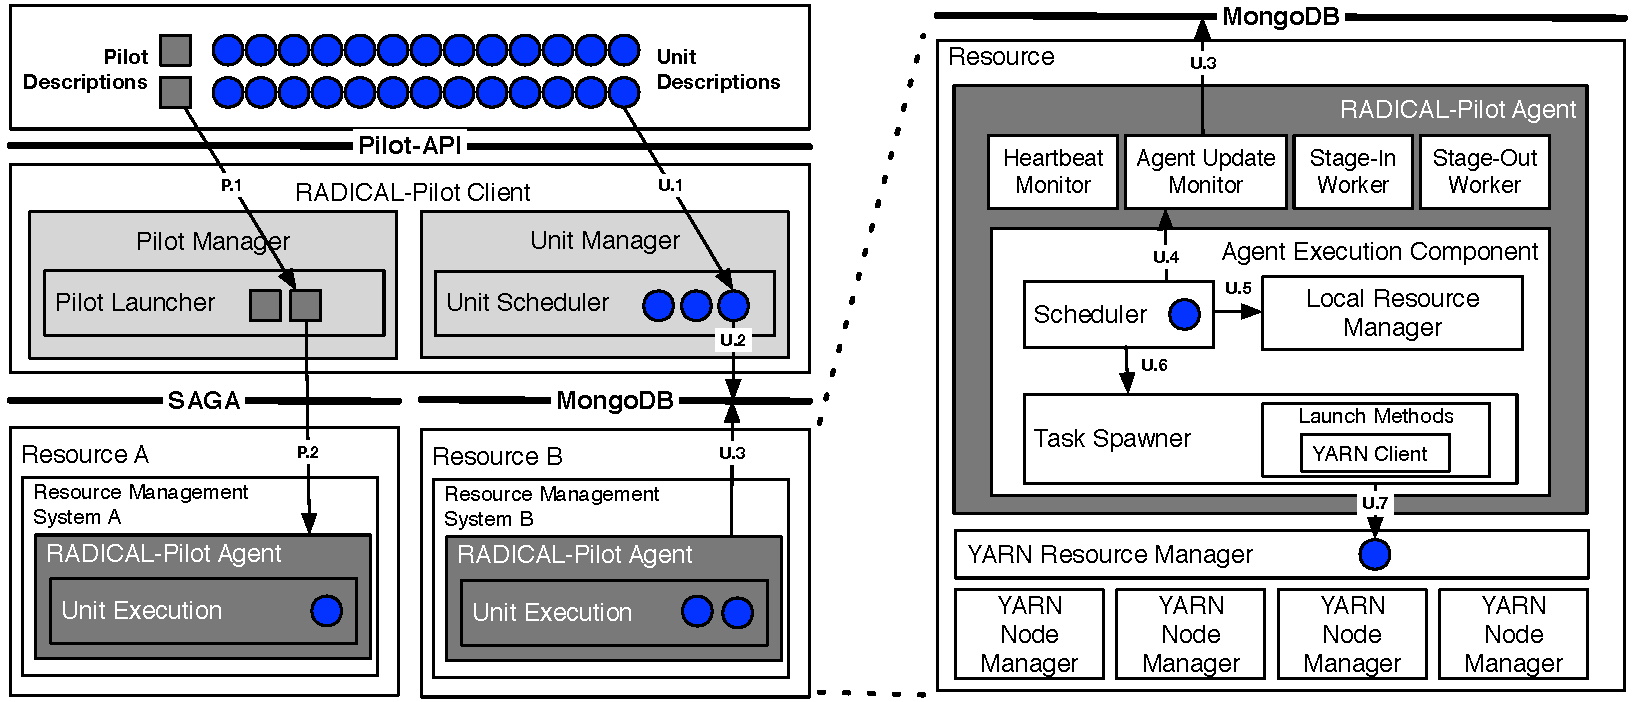
\includegraphics[width=0.85\textwidth]{figures/data_analytics_hpc/hpc_hadoop/rp-architecture-yarn.pdf}
    \caption{\textbf{RADICAL-Pilot and YARN Integration:} There are two main interactions between the application and RADICAL-Pilot -- the management of Pilots (P.1-P.2) and the management of Compute Units (U.1-U.7).  All YARN specifics are encapsulated in the RADICAL-Pilot-Agent.\label{fig:comp_rp_arch}}
\end{figure}

The RADICAL-Pilot-Agent has a modular and extensible architecture and consists of the following components: the Agent Execution Component, Heartbeat Monitor, Agent Update Monitor, Stage In and Stage Out Workers.
The main integration of YARN and RP is done in the Agent Execution Component.
This component consist of four sub-components:
\begin{inparaenum}[a)]
    \item the \textit{scheduler} is responsible for monitoring the resource usage and assigning CPUs/GPUs to Compute Units;
    \item the \textit{Local Resource Manager} (LRM) interacts with the batch system and communicates to the pilot the available number of computing resources and how they are distributed;
    \item the \textit{Task Spawner/ Executor} configures the execution environment, executes and monitors each unit; and
    \item the \textit{Launch Method} encapsulates the environment specifics for executing an application, e.\,g.\ the usage of \texttt{mpiexec} for MPI applications, machine-specific launch methods (e.g. \texttt{aprun} on Cray machines) or the usage of YARN.
\end{inparaenum}
After unit completes its execution, the Task Spawner collects the exit code, standard output, and informs the scheduler about the freed cores.

\subsubsection*{RADICAL-Pilot and YARN Integration}
\label{sssec:rp-yarn}

There are two integration options for RADICAL-Pilot and YARN: (i) Integration on Pilot-Manager level, via a SAGA adaptor, and (ii) integration on the RADICAL-Pilot-Agent level.
The first approach is associated with several challenges: firewalls typically prevent the communication between external machines and a YARN cluster.
A YARN application is not only required to communicate with the resource manager, but also with the node managers and containers.
Further, this approach would require significant extension of the Pilot-Manager, which currently relies on the SAGA Job API for launching and managing pilots.
Capabilities like on-demand provisioning of a YARN cluster and complex application-resource management protocol required by YARN are difficult to abstract behind the SAGA API.

The second approach encapsulates YARN specifics on resource-level and a YARN cluster is decentrally provisioned.
Units are scheduled and submitted to the YARN cluster via the Unit-Manager and the RADICAL-Pilot-Agent scheduler.
By integrating at the RADICAL-Pilot-Agent level, RADICAL-Pilot supports both Mode I and II as outlined in Figure~\ref{fig:figures_hadoop-on-hpc-viceverse}.

As illustrated in Figure~\ref{fig:comp_rp_arch}, RADICAL-Pilot  (steps P.1 and P.2) starts on the remote resource using SAGA.
In Mode I, during the launch of the RADICAL-Pilot-Agent a YARN cluster is spawned on the allocated resources (Hadoop on HPC), while in Mode II the RADICAL-Pilot-Agent connects to a YARN cluster running on the resources of the RADICAL-Pilot-Agent.
Once the RADICAL-Pilot-Agent is started, it accepts Compute Units submitted via the Unit-Manager (step U.1).
The Unit-Manager queues new Compute Units using a shared MongoDB (step U.2).
The RADICAL-Pilot-Agent periodically checks for new Compute Units (U.3) and queues them in the scheduler (U.4).
Finally, the Executor manages the execution of the Compute Units (step U.6 and U.7).

The \emph{Local Resource Manager (LRM)} provides an abstraction to local resource details for other components of the RADICAL-Pilot-Agent.
The LRM evaluates the environment variables provided by the resource management systems to obtain information, such as the number of cores per node, memory and the assigned nodes.
This information can be accessed through the Resource Manager's API.
In Mode I (Hadoop on HPC), during the initialization of the RADICAL-Pilot-Agent, the LRM setups the HDFS and YARN daemons.
First, the LRM downloads Hadoop and creates the necessary configuration files, i.\,e. the \texttt{mapred-site.xml}, \texttt{core-site.xml}, \texttt{hdfs-site.xml}, \texttt{yarn-site.xml} and the slaves and master file containing the allocated nodes.
The node that is running the Agent, runs the master daemons of Hadoop: the HDFS Namenode and the YARN Resource Manager.
After the configuration files are written, HDFS and YARN are started and meta-data about the cluster, i.\,e.\ the number of cores and memory, are provided to the scheduler.
They remain active until all the tasks are executed.
Before termination of the agent, the LRM stops the Hadoop and YARN daemons and removes the associated data files.
In Mode II (Hadoop on HPC), the LRM solely collects the Hadoop cluster resource information.

The \emph{scheduler} is another extensible component of the RADICAL-Pilot-Agent responsible for queuing compute units and assigning them to resources.
To support YARN, we created a special scheduler that utilizes the cluster state information (e.\,g.\ the amount of available cores, memory, queue information, application quotas etc.) obtained via the YARN's Resource Manager's REST API.
In contrast to other RADICAL-Pilot schedulers, it specifically utilizes memory in addition to cores for assigning resources to Compute Units.

The \emph{Task Spawner} is responsible for managing and monitoring the execution of a Compute Unit.
The \emph{Launch Method} component encapsulates resource/launch-method specific operations, e.\,g.\ the usage of the \texttt{yarn} command line tool for submitting and monitoring applications.
After the launch of a Compute Unit, the Task Spawner periodically monitors its execution and updates its state in the shared MongoDB instance by utilizing the application log file.

\begin{figure}[t]
    \centering
    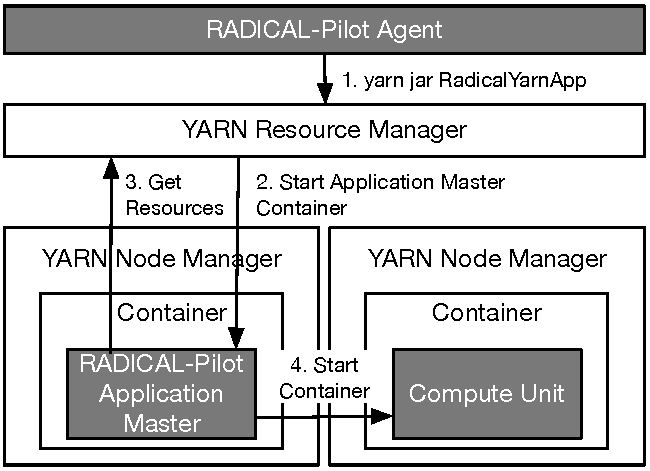
\includegraphics[width=.65\textwidth]{figures/data_analytics_hpc/hpc_hadoop/yarn.pdf}
    \caption{RADICAL-Pilot YARN Agent Application.}
%    \caption{\textbf{RADICAL-Pilot YARN Agent Application: }
%        RADICAL-Pilot provides a YARN application that manages the execution of Compute Units.
%        The application is initialized with parameters defined in the Compute Unit Description and started by the Task Spawner (step 1/2).
%        The Application Master requests resources from the Resource Manager and starts a container running the Compute Unit (step 3/4).}
    \label{fig:figures_yarn}
\end{figure}

\emph{RADICAL-Pilot Application Master:}
A particular integration challenge is the multi-step resource allocation process imposed by YARN depicted in Figure~\ref{fig:figures_yarn}, which differs significantly from HPC schedulers.
The central component of a YARN application is the Application Master, which is responsible for negotiating resources with the YARN Resource Manager as well as managing the execution of an application in the assigned resources.
The unit of allocation in YARN is a container~\cite{murthy2014apache}.
The YARN client (part of the YARN Launch Method) implements a YARN Application Master, which is the central instance for managing the resource requirements of an application.
RADICAL-Pilot utilizes a managed application master that is run inside a YARN container.
Once the Application Master container is started, it is responsible for requesting a YARN container meeting the resource requirements of the Compute Unit from the YARN's Resource Manager.
Once YARN allocates a set of containers, the CU starts inside these containers.
A wrapper script responsible for setting up a RADICAL-Pilot environment, staging of the specified files and running the executable defined in the Compute Unit Description, is used for this purpose.
Every Compute Unit is mapped to a YARN application consisting of an Application Master and a container of the size specified in the Compute Unit Description.

\subsubsection*{RADICAL-Pilot and Spark Integration}
\label{sssec:rp_spark}
Spark offers multiple deployment modes: standalone, YARN and Mesos.
While it is possible to support Spark on top of YARN, this approach is associated with significant complexity and overhead as two instead of one framework need to be configured and bootstrapped.
Since RADICAL-Pilot operates in user-space and single-user mode, no advantages with respect to using a multi-tenant YARN cluster environment exist.
Thus, we support Spark via the standalone deployment mode.

Similar to the YARN integration, the necessary changes for Spark are confined to the RADICAL-Pilot-Agent.
Similarly, the Local Resource Manager is responsible for initialization and deployment of the Apache Spark environment.
In the first step the LRM detects the number of cores, memory and nodes provided by the Resource Management System, verifies and downloads necessary dependencies (e.\,g.\ Java, Scala, and the necessary Spark binaries).
It then creates the necessary configuration files, e.\,g.\ \texttt{spark-env.sh}, \texttt{slaves} and \texttt{master} files, for running a multi-node, standalone Spark cluster.

Finally, the LRM starts the Spark cluster using the previously generated configuration.
Similar to YARN, a Spark RADICAL-Pilot-Agent scheduler is used for managing Spark resource slots and assigning CUs.
During the termination of the RADICAL-Pilot-Agent, the LRM is shutting down the Spark cluster using Spark’s termination script, which stops both the master and the slave nodes.
Similarly, the Spark specific methods for launching and managing Compute Units on Spark are encapsulated in a Task Spawner and Launch Method component.

\section{Experiments and Evaluation}
\label{sec:rph-exps}

To evaluate the RADICAL-Pilot YARN and Spark extension, we conduct two experiments.
In \S~\ref{ssec:startup_pilot_unit}, we analyze and compare RADICAL-Pilot and RADICAL-Pilot-YARN with respect to startup times of both the Pilot and the Compute Units.
We use the well-known K-Means algorithm to investigate the performance and runtime trade-offs of a typical data-intensive application, in \S~\ref{ssec:kmeans}.
Experiments are performed on two different XSEDE allocated machines: Wrangler~\cite{wrangler} and Stampede~\cite{stampede}.
On Stampede every node had 16 cores and 32 GB of memory; on Wrangler 48 cores and 128 GB of memory.
For our experiments we used RADICAL-Pilot v0.45, Hadoop v2.6 and Spark v2.0.2.

\subsection{Pilot Startup and Compute Unit Submission Characterization}
\label{ssec:startup_pilot_unit}

\begin{figure}[t]
    \centering
    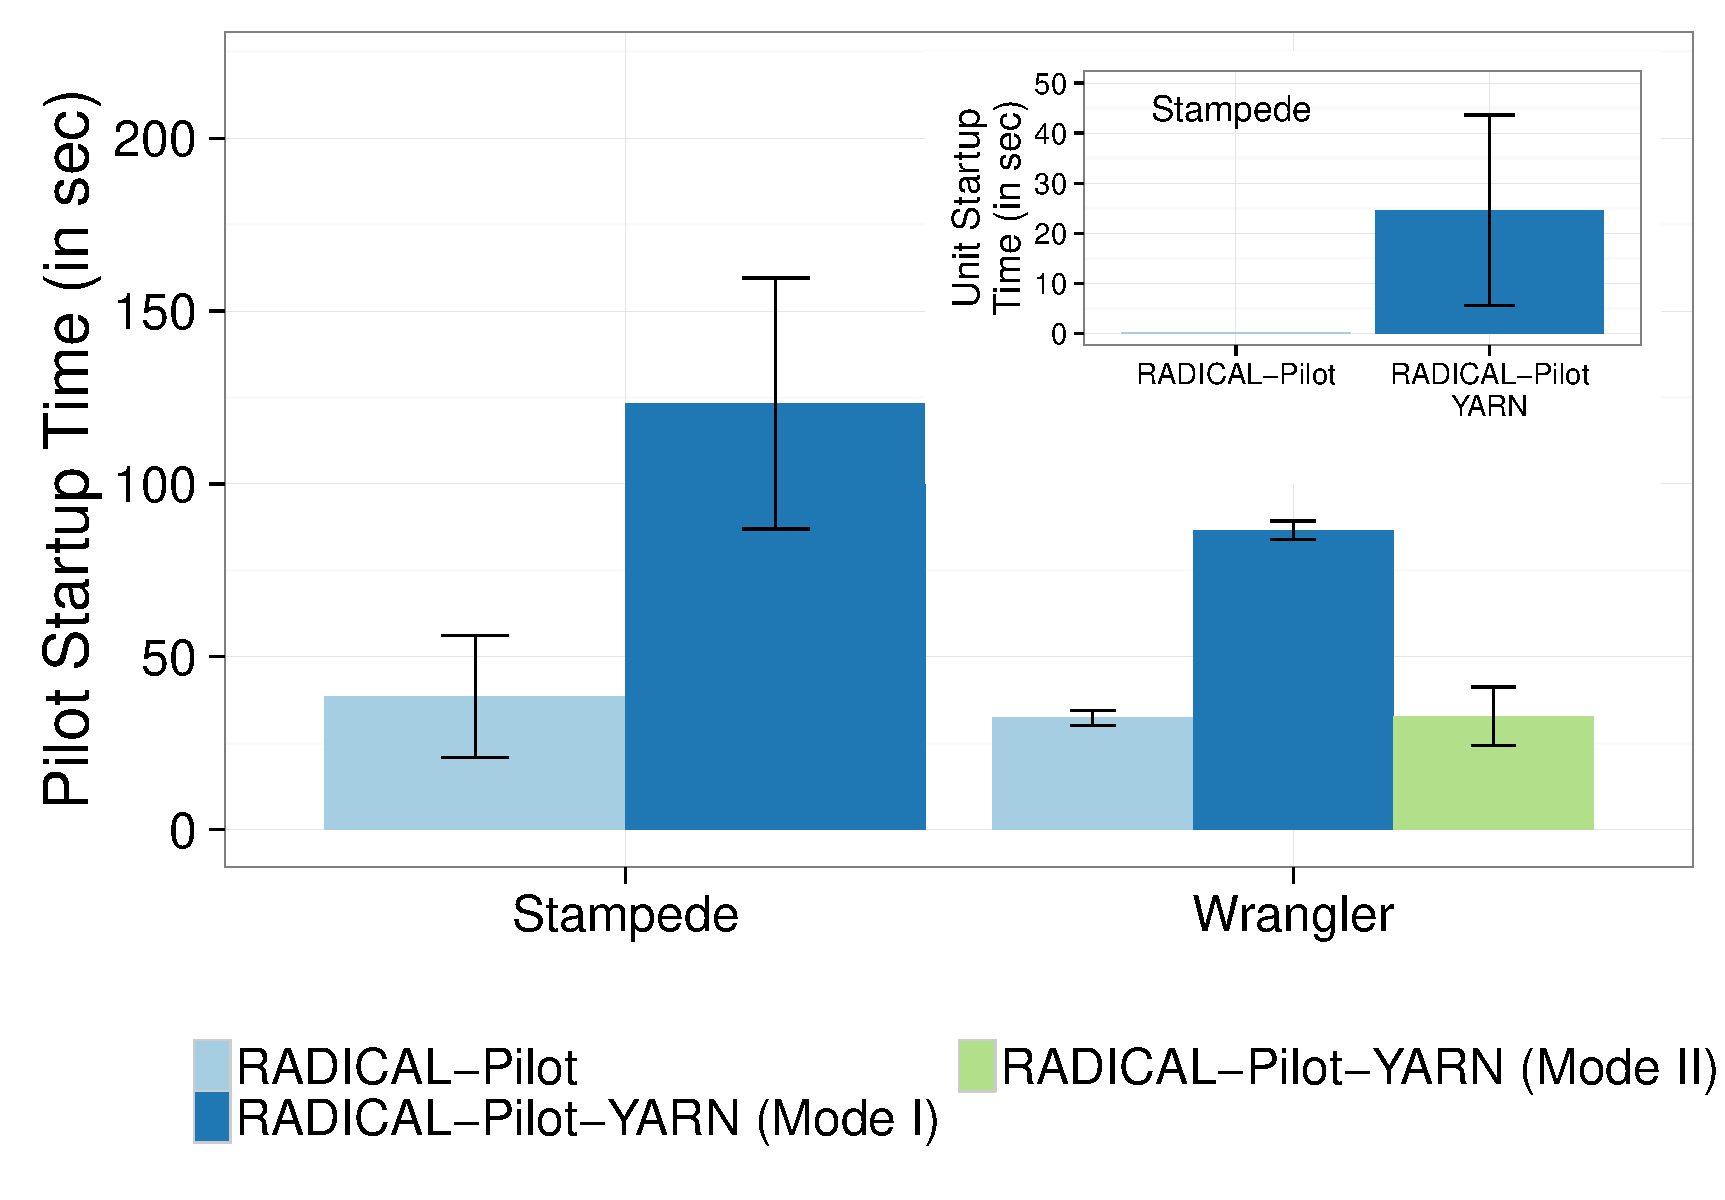
\includegraphics[width=0.75\textwidth]{figures/data_analytics_hpc/hpc_hadoop/pilot_unit_startup.pdf}
    \caption{RADICAL-Pilot and RADICAL-Pilot-YARN startup overheads.
        \label{fig:startup_yarn}}
%    \caption{\textbf{RADICAL-Pilot and RADICAL-Pilot-YARN startup overheads:}
%        The agent startup time is higher for YARN due to the overhead for spawning the YARN cluster.
%        The inset shows that the Compute Unit startup time (time between application submission to YARN and startup) is also significantly higher for YARN.
%        \label{fig:startup_yarn}}
\end{figure}

In Figure~\ref{fig:startup_yarn} we analyze the measured overheads when starting RADICAL-Pilot and RADICAL-Pilot-YARN, and when submitting Compute Units.
The agent startup time for RADICAL-Pilot-YARN is defined as the time between RADICAL-Pilot-Agent starts and the processing of the first Compute Unit.
On Wrangler, we compare both Mode I (Hadoop on HPC) and Mode II (HPC on Hadoop).
For Mode I the startup time is higher compared to the normal RADICAL-Pilot startup time and also compared to Mode II.
This can be explained by the necessary steps required tp download, configure and start the YARN cluster.
For a single node YARN environment, the overhead for Mode I (Hadoop on HPC) is between 50-85\,sec depending upon the resource selected.
The startup times for Mode II on Wrangler -- using the dedicated Hadoop environment provided via the data portal -- are comparable to the normal RADICAL-Pilot startup times as it is not necessary to spawn a Hadoop cluster.

The inset of Figure~\ref{fig:startup_yarn} shows the time taken to start Compute Units via RADICAL-Pilot to a YARN cluster.
For each CU, resources have to be requested in two stages: first the application master container is allocated followed by the containers for the actual compute tasks.
For short-running jobs this represents a bottleneck.

In summary, while there are overheads associated with executing inside of YARN, we believe these are acceptable, in particular for long-running tasks.
The novel capabilities of executing HPC tasks and YARN tasks within the same application has significant benefits for which measured overheads are likely acceptable.

\subsection{K-Means Performance Characterization}
\label{ssec:kmeans}
We compare the time to completion of the K-Means algorithm using two configurations: RADICAL-Pilot on HPC and RADICAL-Pilot in HPC/YARN mode. 
We use three different scenarios: 10,000 points and 5,000 clusters, 100,000 points / 500 clusters and 1,000,000 points / 50 clusters.
Each point belongs to a three dimensional space.
The compute requirements depend on the product of the number of points and clusters, thus it is constant for all three scenarios.
We use an optimized version of K-Means in which the sum and number of points are precomputed in the map phase, thus only these two attributes per cluster need to be shuffled.
The shuffle traffic depends on the number of clusters and decreases with the number of clusters.
For the purpose of this benchmark, we run two iterations of K-Means.

We utilize up to 3 nodes on Stampede and Wrangler.
Experiments are performed with the following configurations: 8 tasks on 1 node, 16 tasks on 2 nodes and 32 tasks on 3 nodes.
For RADICAL-Pilot-YARN, we use Mode II (Hadoop on HPC): the YARN Resource Manager is deployed on the node running the RADICAL-Pilot-Agent.

Figure~\ref{fig:experiments_kmeans_rpyarnkmeans} shows the results of executing K-Means over different scenarios and configurations.
For RADICAL-Pilot-YARN the runtimes include the time required to download and start the YARN cluster on the allocated resources.

\begin{figure}[t]
    \centering
    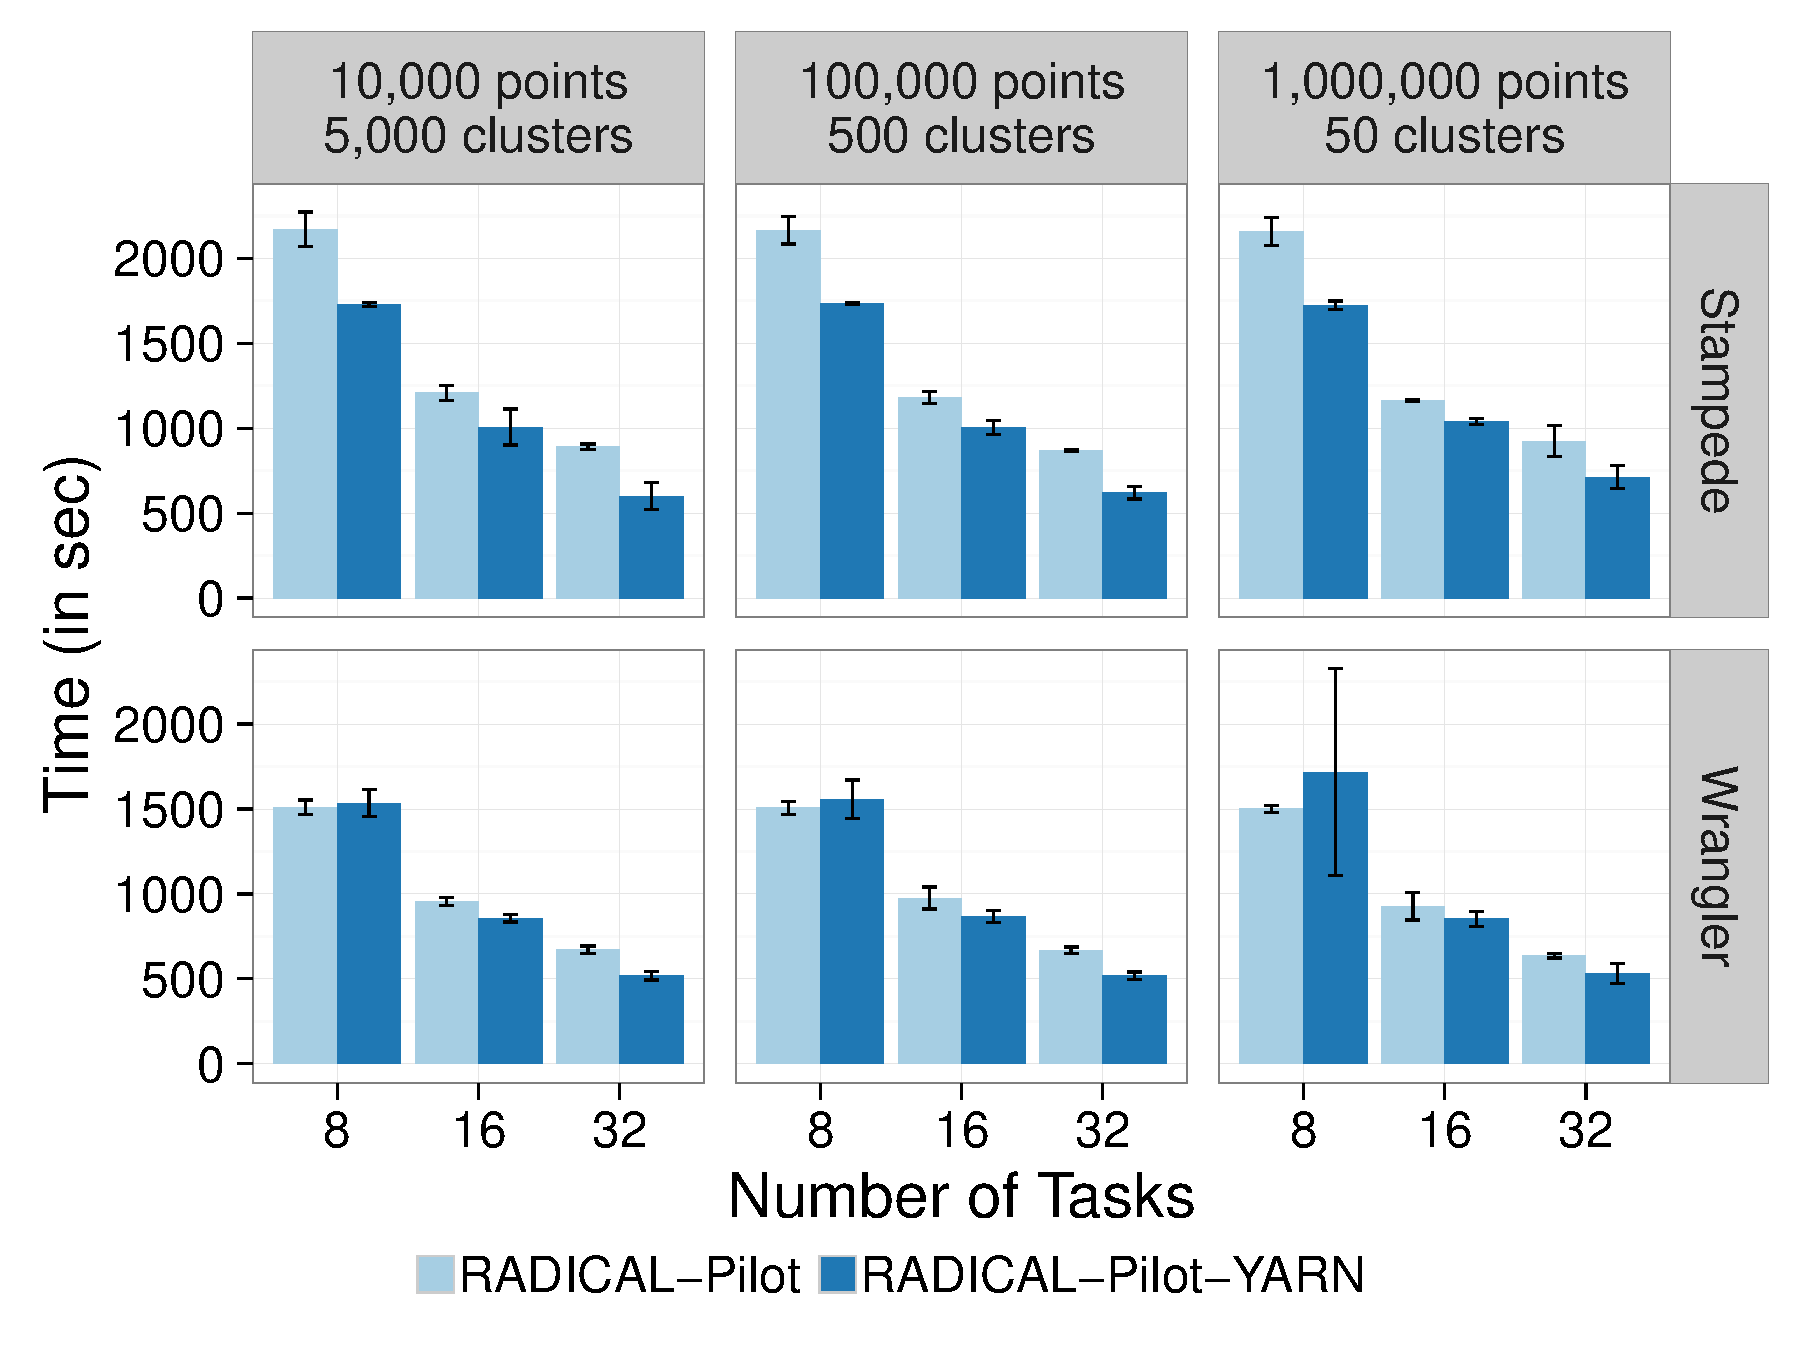
\includegraphics[width=.75\textwidth]{figures/data_analytics_hpc/hpc_hadoop/kmeans.pdf}
    \caption{RADICAL-Pilot and YARN-based K-Means time to completion on Stampede and Wrangler.}
%\caption{\textbf{RADICAL-Pilot and YARN-based K-Means on Stampede and Wrangler:}
%        Across all configurations the performance of the YARN backend is in average 13\,\% better.
%        On Wrangler a significant better performance and scalability (higher speedups) were observed.}
    \label{fig:experiments_kmeans_rpyarnkmeans}
\end{figure}

Independent of the scenario, the runtimes decrease with the number of tasks.
In particular, in the 8 task scenarios the overhead of YARN is visible on Wrangler.
For larger number of tasks, we observed on average 13~\% shorter runtimes for RADICAL-Pilot-YARN.
Also, RADICAL-Pilot-YARN achieves better speedups, e.\,g., 3.2 for 32 tasks for the 1 million points scenario, which is significantly higher than the RADICAL-Pilot speedup of 2.4 (both on Wrangler and compared to base case of 8 tasks).
One of the reasons is that for RADICAL-Pilot-YARN uses the local file system, while for RADICAL-Pilot uses the Lustre filesystem.

For similar scenarios and task/resource configuration, the runtimes on Wrangler show a significant performance improvements over Stampede.
This is attributed to the better hardware (CPUs, memory) of Wrangler than Stampede.
In particular for RADICAL-Pilot-YARN we observed on average higher speedups on Wrangler, indicating that we saturated the 32 GB of memory available on each Stampede node.

In summary, despite the overheads of RADICAL-Pilot-YARN with respect to Pilot and Compute Unit startup time, we were able to observe performance improvements (on average 13~\% better time to completion) mainly due to the better performance of the local disks.


\section{Conclusions}
\label{sec:hpc_hadoop_concl}
Hadoop and Spark are used by increasing number of scientific applications mainly due to accessible abstractions they provide.
HPC and Hadoop environments are converging, for example, MLLib/Spark utilize BLAS, Hadoop frameworks adopt parallel and in-memory computing concepts that originated in HPC.
Currently, traditional HPC applications lack the ability to access and use Hadoop and other Hadoop tools, without sacrificing the advantages of HPC environments.
One prominent reason behind the limited uptake, is finding effective and scalable resource management techniques usable for Hadoop frameworks on HPC infrastructure.

This chapter motivates the use of the Pilot-Abstraction as an integrating concept, discusses the design and implementation of RADICAL-Pilot extensions for Hadoop and Spark, and validates them with scalability analysis on two supercomputers.
Our experiments use RADICAL-Pilot, and introduce two extensions to RADICAL-Pilot to better integrate Hadoop on HPC.
We demonstrate that the Pilot-Abstraction strengthens the state of practice in utilizing HPC resources in conjunction with emerging Hadoop frameworks by allowing users to combine a diverse set of best-of-breed tools running on heterogeneous infrastructure consisting of HPC.
Using these capabilities, complex data campaigns can utilize a diverse set of Hadoop and HPC frameworks enabling scalable data ingests and analytics workflows.
Providing both a unifying and powerful abstraction that enables all parts of such a data pipeline to co-exist is critical.

While we demonstrated the importance of integrated capabilities for supporting data analytics on HPC, we want to understand their performance impact on scientific task-based data analytics scientific workflows.
This is important when executing computational campaigns on HPC resources, as selecting a suitable capability to execute data-intensive workflows is desirable.
Thus, we continue our work with integrating and measuring the performance of molecular dynamics data-analysis workflows utilizing these capabilities on HPC resources.

%%%%%%%%%%%%%%%%%%%%%%%%%%%%%%%%%%%%%%%%%%%%%%%%%%%%%%%%%%%%%%%%%%%%%%%%%%%%%%%%
%
%For example, Cray's analytics platform Urika~\footnote{http://www.cray.com/products/analytics} has Hadoop and Spark running on HPC architecture as opposed to regular clusters, but without the HPC software environment and capabilities.
%However, several applications ranging from bio-molecular simulations to epidemiology models~\cite{network1} require significant simulations interwoven with analysis capabilities such as clustering and graph analytics; in other words some stages (or parts of the same stage) of an application would ideally utilize Hadoop/Spark environments and other stages (or parts thereof) utilize HPC environments.
%
%Over the past decades, the High Performance Distributed Computing (HPDC) community has made significant advances in addressing resource and workload management on heterogeneous resources.
%For example, the concept of multi-level scheduling~\cite{1392910} as manifested in the decoupling of workload assignment from resource management using the concept of intermediate container jobs (also referred to as \pilotjobs~\cite{pstar12}) has been adopted for both HPC and Hadoop.
%Multi-level scheduling is a critical capability for data-intensive applications as often only application-level schedulers can be aware of the localities of the data sources used by a specific application.
%This motivated the extension of the \pilot-Abstraction to \pilotdata~\cite{pilot-data-jpdc-2014} to form the central component of a resource management middleware.
%
%In the following sections, we discuss a set of tools for supporting both of these usage modes:
%In section~\ref{ssec:saga_hadoop} we present SAGA-Hadoop, a light-weight tool for running Hadoop on HPC (Mode I).
%We then discuss, the integration of Hadoop and Spark runtimes into RADICAL-Pilot, which enables both the interoperable use of HPC and Hadoop, as well as the integration of HPC and Hadoop applications (Mode I and II) (Section~\ref{ssec:rp-impl}).
%Using these new capabilities, applications can seamlessly connect HPC stages (e.\,g.\ simulation stages) with analysis staging using the Pilot-Abstraction to provide unified resource management.
%
%\subsection{Mode I: SAGA-Hadoop, supporting Hadoop/Spark on HPC}
%\label{ssec:saga_hadoop}
%
%SAGA-Hadoop~\cite{saga-hadoop} is a tool for supporting the deployment of Hadoop and Spark on HPC resources (Mode I in Figure~\ref{fig:figures_hadoop-on-hpc-viceverse}).
%Using SAGA-Hadoop an applications written for YARN (e.\,g.\ MapReduce) or Spark (e.\,g. PySpark, DataFrame and MLlib applications) can be executed on HPC resources.
%
%Figure~\ref{fig:saga-hadoop} illustrates the architecture of SAGA-Hadoop.
%SAGA-Hadoop uses SAGA~\cite{merzky2015saga} to spawn and control Hadoop clusters inside an environment managed by an HPC scheduler.
%SAGA is used for dispatching a bootstrap process that generates the necessary configuration files and starting Hadoop.
%The specifics of the Hadoop framework (i.\,e.\ YARN and Spark) are encapsulated in a Hadoop framework plugin (also referred to as adaptors).
%SAGA-Hadoop delegates tasks, such as the download, configuration and start of a framework to this plugin.
%In the case of YARN, the plugin is then responsible for launching YARN's Resource and Node Manager processes; in the case of Spark, the Master and Worker processes.
%This architecture is extensible as new frameworks, e.\,g.\ Flink, can easily be added.
%
%\begin{figure}[t]
%    \centering
%    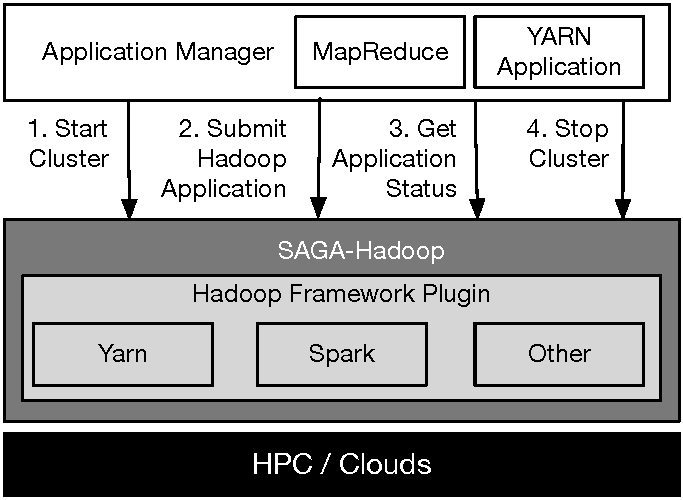
\includegraphics[width=.95\textwidth]{figures/data_analytics_hpc/hpc_hadoop/pilot-abds.pdf}
%    \caption{SAGA-Hadoop for HPC and Cloud Infrastructures.}
%    \label{fig:saga-hadoop}
%\end{figure}
%
%While nearly all Hadoop frameworks (e.\,g.\ MapReduce and Spark) support YARN for resource management, Spark provides a standalone cluster mode, which is more efficient in particular on dedicated resources.
%Thus, a special adaptor for Spark is provided.
%Once the cluster is setup, users can submit applications using SAGA's API that allows them to start and manage YARN or Spark application processes.
%
%While SAGA-Hadoop provides the interoperability between YARN and HPC resources by treating YARN as a substitute for common HPC schedulers, the integration of YARN and HPC applications or application stages remains challenging.
%As a consequence, we explored the usage of the Pilot~-Abstraction~\cite{luckow2012pstar}, through RADICAL-Pilot~\cite{merzky2019using}, to enable the integration between these different application types.

% ---------------------------------------------------------
% CHAPTER 3
% ---------------------------------------------------------
\chapter{Task-Parallel Data Analytics on HPC Platforms}
\label{ch:task-par}
\label{sec:task-par}

Data based workflow engines exploit task-parallelism by partitioning the data and generating stages of independent tasks.
These stages then ordered and implement data dependencies by shuffling, aggregating or coupling intermediate results.
The MapReduce~\cite{dean2004mapreduce} abstraction, along with its implementations, popularized this method of processing.

Spark~\cite{zaharia2010spark} and Dask~\cite{rocklin2015dask} are two Big Data frameworks.
Both provide MapReduce abstractions and are optimized for parallel processing of large data volumes, interactive analytics and machine learning.
Their runtime engines can automatically partition data, generate parallel tasks, and execute them on a cluster.
In addition, Spark offers in-memory capabilities allowing caching data that are read multiple times, making it suited for interactive analytics and iterative machine learning algorithms.
Dask also provides a MapReduce API (Dask Bags).
Furthermore, Dask's API is more versatile, allowing custom workflows and parallel vector/matrix computations.

\section{Molecular Dynamics (MD) Data Analysis}
%\label{ssec:use_cases}
Some commonly used algorithms for analyzing MD trajectories are Root Mean Square Deviation (RMSD), Pairwise Distances (PD), and Sub-setting~\cite{mura2014biomolecules}.
Two more advanced algorithms are Path Similarity Analysis (PSA)~\cite{seyler2015path} and Leaflet Identification~\cite{michaud2011mdanalysis}.
RMSD is used to identify the deviation of atom positions between frames.
PD and PSA methods calculate distances based on different metrics either between atoms or trajectories.
Sub-setting methods are used to isolate parts of interest of MD simulation.
Leaflet Identification provides information about groups of lipids by identifying the lipid leaflets in a lipid bilayer.
All these methods, in some way, read and process the whole physical system generated via simulations.
The analysis reduces the data to either a number or a matrix.

We discuss two of these methods, a Path Similarity Analysis (PSA) algorithm using the Hausdorff distance and a Leaflet Identification method, and their implementations in MDAnalysis~\cite{michaud2011mdanalysis,gowers2016mdanalysis}.
Section~\ref{ssec:mda} discusses the reasons for selecting these two algorithms in more detail.
%In addition, we implemented the PSA algorithm using CPPTraj~\cite{roe2013ptraj}.
%Furthermore, we explore the applications' Ogres Facets and Views~\cite{fox2014towards}, which provide a more systematic characterization.

%Big Data Ogres~\cite{fox2014towards} are organized into four classes, called \emph{views}.
%The possible features of a view are called \emph{facets}.
%A combination of facets from all views defines an Ogre.
%The Views are: 
%\begin{inparaenum}[1)]
%    \item execution - describes aspects, such as I/O, memory, compute ratios, whether computations are iterative, and the 5 V's of Big Data (Volume, Velocity, Value, Variety and Veracity),
%    \item data source \& style - discusses input data collection, storage and access,
%    \item processing - describes algorithms and kernels used for computation, and
%    \item problem architecture - describes the application architecture.
%\end{inparaenum}


\subsection{Applications and Algorithms: MDAnalysis}
\label{ssec:mda}
MDAnalysis is a Python library~\cite{michaud2011mdanalysis,gowers2016mdanalysis} that provides a comprehensive environment for filtering, transforming and analyzing MD trajectories in all commonly used file formats.
It provides a common object-oriented API to trajectory data and leverages existing libraries in the scientific Python software stack, such as NumPy~\cite{numpy} and Scipy~\cite{scipy}.

\subsubsection*{Path Similarity Analysis (PSA): Hausdorff Distance}Path Similarity Analysis (PSA)~\cite{seyler2015path} is used to quantify the similarity between trajectories considering their full atomic detail.
The basic idea is to compute pair-wise distances (for instance, using the Hausdorff metric~\cite{huttenlocher1993comparing}) between members of an ensemble of trajectories and cluster the trajectories based on their distance matrix.

Each trajectory is represented as a two dimensional array.
The first dimension corresponds to time frames of the trajectory, the second to the $N$ atom positions, in 3-dimensional space.

\begin{algorithm}[t]
    \scriptsize
    \caption{Path Similarity Algorithm: Hausdorff Distance}
    \label{alg:hausdorff}
    \begin{algorithmic}[1]
        \Procedure{HausdorffDistance}{$T_1$,$T_2$}\Comment{$T_1$ and $T_2$ are a set of 
            3D points}
        \State \texttt{List $D_1$,$D_2$}
        \For{$\forall frame_1$ in $T_1$}
        \For{$\forall frame_2$ in $T_2$}
        \State \texttt{Append in $D_1$ $d_{RMS}$($frame_1$, $frame_2$)}
        \EndFor
        \State \texttt{$D_{t_1}$ append $min(D_1)$}
        \EndFor
        \For{$\forall frame_2$ in $T_2$}
        \For{$\forall frame_1$ in $T_1$}
        \State \texttt{Append in $D_2$ $d_{RMS}$($frame_2$, $frame_1$)}
        \EndFor
        \State\texttt{$D_{t_2}$ append $min(D_2)$}
        \EndFor
        \State \textbf{return} $max\Big(max(D_{t_1}),max(D_{t_2})\Big)$
        \EndProcedure
        \\        
        \Procedure{PSA}{$Traj$}\Comment{$Traj$ is a set of trajectories}
        \For{$\forall T_1$ in $Traj$}
        \For{$\forall T_2$ in $Traj$}
        \State \texttt{ $D_{( T_1,T_2 )}$=HausdorffDistance$\Big( T_1,T_2 \Big)$} 
        \EndFor
        \EndFor
        \State \Return $D$
        \EndProcedure
    \end{algorithmic}
\end{algorithm}

Algorithm~\ref{alg:hausdorff} describes the PSA algorithm with the Hausdorff metric over multiple trajectories.
We apply a 2-dimensional data partitioning over the output matrix to parallelize, shown in algorithm~\ref{alg:partition}.
Our Hausdorff metric calculation is based on a naive algorithm.
Recently, an algorithm was introduced that uses early break to speedup execution~\cite{taha2015efficient}, although we are not aware of a parallel implementation of this algorithm.

\begin{algorithm}[t]
    \scriptsize
    \caption{Two Dimensional Partitioning}
    \label{alg:partition}
    \begin{algorithmic}[1]
        \State Initially, there are $N^2$ distances, where $N$ is the number of trajectories.
        Each distance defines a computation task.
        \State Map the initial set to a smaller set with $k=N/n_1$ elements, where $n_1$ is a divisor of $N$, by grouping $n_1$ by $n_1$ elements together.
        \State Execute over the new set with $k^2$ tasks.
        Each task is the comparisons between $n_1$ and $n_1$  elements of the initial set.
        They are executed serially.
    \end{algorithmic}
\end{algorithm}

The algorithm is embarrassingly parallel and uses linear algebra kernels for calculations.
It has complexity $O(n^2)$ (problem architecture \& processing views).
Input data volume is medium to large while the output is small.
Specific execution environments, such as HPC nodes, and Python arithmetic libraries, e.g., NumPy, are used (execution view).
Input data are produced by HPC simulations, and are stored on HPC storage systems, such as parallel filesystem like Lustre (data source \& style view).

Embarrassingly parallel algorithms are good candidates to utilize task parallelization.
The data are partitioned to independent parts and each part is assigned to a task.
These tasks can then execute as a bag of tasks.
As a result, they are ideally suited for task-management and MapReduce APIs.
They can be expressed as a bag of tasks using a task management API or a map-only application in a MapReduce-style API.
All three selected frameworks support the execution of bag of tasks, with RADICAL~-Pilot and Dask offering specific abstractions (as discussed in \S~\ref{ssec:frameworks}).

\subsubsection*{Leaflet Finder}Algorithm~\ref{alg:leafletfinder} describes the Leaflet Finder (LF) algorithm as presented in Ref.~\cite{michaud2011mdanalysis}.
LF assigns particles to one of two curved but locally approximately parallel sheets, provided that the inter-particle distance is smaller than the distance between sheets.
In biomolecular simulations of lipid membranes, consisting of a double layer of lipid molecules, LF is used to identify the lipids in the outer and inner leaflets (sheets).
The algorithm consists of two stages:
\begin{inparaenum}[a)]
    \item construction of a graph connecting particles based on threshold distance (cutoff), and
    \item computing the connected components of the graph, determining the lipids located on the outer and inner leaflets.
\end{inparaenum}

\begin{algorithm}[t]
    \scriptsize
    \caption{Leaflet Finder Algorithm}
    \label{alg:leafletfinder}
    \begin{algorithmic}[1]
        \Procedure{LeafletFinder}{$Atoms,Cutoff$}
        \Comment{$Atoms$ is a set of 3D points that represent the position of atoms in space. $Cutoff$ is an Integer Number}
        \State \texttt{Graph G =$(V=Atoms,E=\emptyset)$}
        \For{$\forall atom$ in $Atoms$}
        \State \texttt{$N = [a\in V: d(a,atom)\le Cutoff]$}
        \State \texttt{Add edges $[(atoms,a): a \in N]$ in G}
        \EndFor
        \State \texttt{C = ConnectedComponents(G)}
        \State \Return C
        \EndProcedure
    \end{algorithmic}
\end{algorithm}

The application stages have different complexities.
The first stage identifies neighboring atoms.
There are different implementation alternatives: 
\begin{inparaenum}[i)]
    \item computing the distance between all atoms ($O(n^2)$);
    \item utilizing a tree-based nearest neighbor (Construction: $O(n\log n)$, 
    Query: $O(\log n)$).
\end{inparaenum}
In both alternatives the input data volume is medium size and the output is smaller than the input.
The complexity of connected components is: $O(|V|+|E|)$ ($V$: Vertices, $E$: Edges), i.\,e. it greatly depends on the characteristics of the graph.

The application typically uses HPC nodes as the execution environment, and NumPy arrays (execution view).
It uses matrices to represent the physical system and the distance matrix.
The output data representation is a graph.
Leaflet Finder can be efficiently implemented using the MapReduce abstraction (problem architecture view).
It uses graph algorithms and linear algebra kernels (processing view facets).
The data source \& style view facets are the same as the PSA algorithm.

Leaflet Finder is more complex as it requires two stages.
It is possible to implement Leaflet Finder with a simple task-management API, although the MapReduce programming model allows more efficient implementation with a \texttt{map} for computing and filtering distances and a \texttt{reduce} for finding the components.
The shuffling required between map and reduce is medium as the number of edges is a fraction of the input data.
Spark and Dask natively support MapReduce and implementinf the Leaflet Finder algorithm is relatively straightforward.
RADICAL-Pilot, on the other hand, does not support natively MapReduce.
As a result, it is required by the application developer to define the data shuffling between the \emph{map} and \emph{reduce} phase of the algorithm.

%\subsubsection{CPPTraj}
%CPPTraj~\cite{roe2013ptraj,roe2018parallelization} is a C++ MD trajectory analysis tool.
%It is parallelized via MPI and OpenMP.
%CPPtraj reads in parallel frames from a single trajectory file or ensemble members of the same trajectory from different files.
%The frames are equally distributed to the MPI processes.
%Computational intensive algorithms are further parallelized using OpenMP.
%It requires at least one MPI process per ensemble member, where each member is a single trajectory file.


\subsection{Current Solutions for Parallel MD Data Analysis}
\label{ssec:related_work}
MD analysis algorithms were until recently executed serially and parallelization was not straightforward.
During the last years several frameworks emerged providing parallel algorithms for analyzing MD trajectories.
Some of those frameworks are CPPTraj~\cite{roe2013ptraj,roe2018parallelization}, HiMach~\cite{tiankai2008scalable}, PMDA~\cite{fan2019pmda}, Pteros 2.0~\cite{yesylevskyy2015pteros} and nMoldyn-3~\cite{hinsen2012nmoldyn}.
%We compare these frameworks with our approach over the parallelization techniques used.

Several different techniques are used for parallelizing these algorithms.
CPPTraj~\cite{roe2018parallelization} utilizes MPI and OpenMP to exeucte large scale analysis on HPC.
OpenMP is also utilized by Pteros~\cite{yesylevskyy2015pteros} to parallelize the compute intensive parts of the analysis.
HiMach~~\cite{tiankai2008scalable} extends Google's MapReduce and defines Map and Reduce methods.
nMoldyn-3~\cite{hinsen2012nmoldyn} parallelizes the execution through a Master Worker architecture.
The master defines analysis tasks, submits them to a task manager, which then are executed by the worker process.

%HiMach~\cite{tiankai2008scalable} was developed by D. E. Shaw Research group to provide a parallel analysis framework for MD simulations, and extends Google's MapReduce.
%HiMach API defines trajectories, does per frame data acquisition (Map) and cross-frame analysis (Reduce).
%HiMach's runtime is responsible to parallelize and distribute Map and Reduce phases to resources.
%Data transfers are done through a communication protocol created specifically for HiMach.

%Pteros-2.0~\cite{yesylevskyy2015pteros} is a open-source library that is used for modeling and analyzing MD trajectories, providing a plugin for each supported algorithm.
%The execution is done by a user defined driver application, which setups trajectory  I/O and frame dispatch for analysis.
%It offers a C++ and Python API.
%Pteros 2.0 parallelizes computational intensive algorithms via OpenMP and Multithreading.
%As a result, it is bounded to execute on a single node, making any analysis execution highly dependent on memory size.
%Through RADICAL-Pilot, Spark and Dask, we avoided recompiling every time there is a change to the underlying resource, ensuring the application's execution.

%MDTraj~\cite{mcgibbon2015mdtraj} is a Python package for analyzing MD trajectories.
%It links MD data and Python statistical and visualization software.
%MDTraj proposes parallelizing the execution by using the parallel package of IPython as a wrapper along with an out-of-core trajectory reading method.
%Our approach allows data parallelization on any level of the execution, not only in data read.

%nMoldyn-3~\cite{hinsen2012nmoldyn} parallelizes the execution through a Master Worker architecture.
%The master defines analysis tasks, submits them to a task manager, which then are executed by the worker process.
%In addition, it provides adaptability, allowing on-the-fly addition of resources, and execution fault tolerance when worker processes disconnect.

A common denominator of most approaches is that they do not use general purpose frameworks for parallelizing the execution.
Although, they are optimized to get as much performance as possible from the environments they are developed for, their portability is limited.
CPPTraj~\cite{roe2018parallelization} and Pteros~\cite{yesylevskyy2015pteros}, for example, are highly dependent on the underlying low level libraries of the resource they use.
HiMach~\cite{tiankai2008scalable} is build specifically for the Antons Supercomputer.

In contrast, our approach and PMDA~\cite{fan2019pmda} utilize more general purpose frameworks for parallelization.
Specifically, PMDA utilizes Dask to parallelize MD Trajectory analysis.
The frameworks used provide higher level abstractions, e.g machine learning, so any  integration with other data analysis methods can be fast and easier.
In addition, resource acquisition and management is done transparently.

\section{Task-Parallel Frameworks: RADICAL-Pilot, Spark, Dask}
\label{ssec:frameworks}
The landscape of frameworks for data-intensive applications is manifold~\cite{jha2014tale,kamburugamuve2017anatomy} and has been extensively studied in the context of scientific~\cite{jha2017introducing} applications.
In this section, we discuss the suitability of frameworks such as Spark~\cite{zaharia2010spark}, Dask~\cite{rocklin2015dask} and RADICAL~-Pilot~\cite{merzky2019using}, for MD data analytics.

\subsection{Background}
%MapReduce~\cite{dean2004mapreduce} and its open source Hadoop implementation combined a simple functional API with a powerful distributed computing engine that exploits data locality to allow optimized I/O performance.
%However, MapReduce is inefficient for interactive workloads and iterative machine learning algorithms~\cite{zaharia2010spark,ekanayake2010twister}.
Spark and Dask provide rich APIs, caching and other capabilities critical for analytics applications.
Spark is considered the standard solution for iterative data-parallel applications.
Dask is quickly gaining support in the scientific community, since it offers a fully python environment.
RADICAL~-Pilot is a Pilot-Job framework~\cite{luckow2012pstar} that supports task-level parallelism on HPC resources and adds a parallelization level on top of HPC MPI-based applications.
%RADICAL~-Pilot is a Pilot-Job framework~\cite{luckow2012pstar} that supports task-level parallelism on HPC resources.
%It successfully adds a parallelization level on top of HPC MPI-based applications.

As described in~\cite{jha2014tale}, these frameworks typically comprise of distinct layers, e.\,g.,cluster scheduler access, framework-level scheduling, and higher-level abstractions.
On top of low-level resource management capabilities various higher-level abstractions can be provided, e.\,g., MapReduce-inspired APIs.
These then provide the foundation for analytics abstractions, such as Dataframes, Datasets and Arrays.
Figure~\ref{fig:figures_bigdata_framework_stack} visualizes the different components of RADICAL~-Pilot, Spark and Dask.
The following describes each framework in detail.

\begin{figure}[ht]
    \centering
    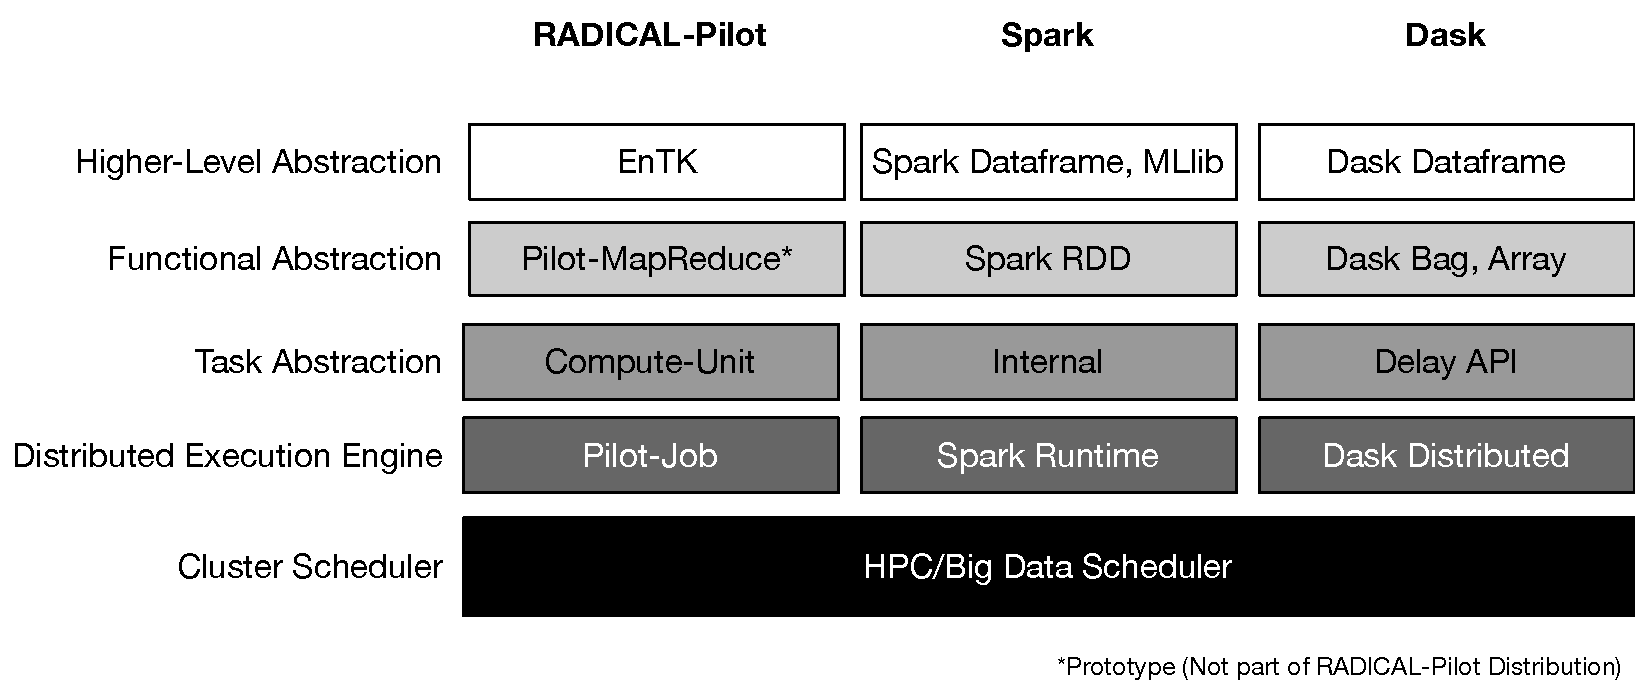
\includegraphics[width=.95\textwidth]{figures/data_analytics_hpc/task_par/bigdata_framework_stack.pdf}
    \caption{Architecture of RADICAL~-Pilot, Spark and Dask.}
    %\caption{\textbf{Architecture of RADICAL~-Pilot, Spark and Dask:}
    %The frameworks share common architectural components for managing cluster resource, and tasks.
    %Spark, Dask offer several high-level abstractions inspired by MapReduce.}
    \label{fig:figures_bigdata_framework_stack}
\end{figure}

\subsubsection*{RADICAL-Pilot}
%RADICAL~-Pilot~\cite{merzky2019using} is a Pilot system that implements the pilot paradigm as outlined in Ref.~\cite{turilli2018comprehensive}.
%RADICAL~-Pilot (RP) is implemented in Python and provides a well defined API and usage modes.
%Although RP is vehicle for research in scalable computing, it also supports production grade science.
%Currently, it is being used by applications drawn from diverse domains, ranging from earth and biomolecular sciences to high-energy physics.
%RP can be used as a runtime system by workflow or workload management systems~\cite{turilli2019middleware,treikalis2016repex,balasubramanian2018harnessing,dakka2018high,turilli2017evaluating}.
%In 2017, RP was used to support more than 100M core-hours on US DOE, NSF resources (BlueWaters and XSEDE), and European supercomputers (Archer and SuperMUC).

As discussed in \S~\ref{sec:pilot-data-hadoop}, RADICAL~-Pilot allows concurrent task execution on HPC resources.
The user defines a set of Compute~-Units (CU)~- the abstraction that defines a task along with its dependencies - which are submitted to RADICAL~-Pilot.
RADICAL~-Pilot schedules these CUs to be executed under the acquired resources.
It uses the existing environment of the resource to execute tasks.
Any data communication between tasks is done via an underlying shared filesystem, e.g., Lustre.
Task execution coordination and communication is done through a database (MongoDB).

%RADICAL~-Pilot's learning curve can be quite steep at the beginning, at least until the user becomes familiar with the concept and usability of Pilots and CUs.
%Once the user is comfortable with RADICAL~-Pilot's API, she can easily develop new algorithms.

\subsubsection*{Spark}
Spark~\cite{zaharia2010spark} extends MapReduce~\cite{dean2004mapreduce} providing a rich set of operations on top of the Resilient Distributed Dataset (RDD) abstraction~\cite{zaharia2012resilient}.
RDDs are cached in-memory making Spark well suitable for iterative applications that need to cache a set of data across multiple stages.
PySpark provides a Python API to Spark.

A Spark job is compiled of multiple stages; a stage is a set of parallel tasks executed without communicating (e.\,g., \texttt{map}) and an action (e.\,g., \texttt{reduce}).
Each action defines new stage.
The \texttt{DAGScheduler} is responsible for translating the workflow specified via RDD transformations and actions to an execution plan.
Spark's distributed execution engine handles the low-level details of task execution.
The execution of a Spark job is triggered by actions.
Spark can read data from different sources, such as HDFS, blob storage, parallel and local filesystems.
While Spark caches loaded data in memory, it offloads to disk when an executor does not have enough free memory to hold all the data of its partition.
Persisted RDDs remain in memory, unless specified to use the disk either complementary or as a single target.
In addition, Spark writes to disk data that are used in a shuffle.
As a result, it allows quick access to those data when transmitted to an executor.
Finally, Spark provides a set of actions that write text files, Hadoop sequence files or object files to local filesystems, HDFS or any filesystem that supports Hadoop.
In addition, Spark supports higher-level data abstractions for processing structured data, such as dataframes, Spark-SQL, datasets, and data streams.

\subsubsection*{Dask}
Dask~\cite{rocklin2015dask} provides a Python-based parallel computing library, which is designed to parallelize native Python code written for NumPy and Pandas.
In contrast to Spark, Dask also provides a lower-level task API (\texttt{delayed} API) that allows users to construct arbitrary workflow graphs.
Being written in Python, it does not require to translate data 
types from one language to another like PySpark, which moves data between Python's interpreter and Java/Scala.

In addition to the low-level task API, Dask offers three higher-level abstractions: Bags, Arrays and Dataframes.
Dask Arrays are a collection of NumPy arrays organized as a grid.
Dask Bags are similar to Spark RDDs and are used to analyze semi-structured data, like JSON files.
Dask Dataframe is a distributed collection of Pandas dataframes that can be analyzed in parallel.

Furthermore, Dask offers three schedulers: multithreading, multiprocessing and distributed.
The multithreaded and multiprocessing schedulers can be used only on a single node and the parallel execution is done via threads and processes respectively.
The distributed scheduler creates a cluster with a scheduling process and multiple worker processes.
A client process creates and communicates a DAG to the scheduler.
The scheduler assigns tasks to workers.

Dask's learning curve cannot be considered steep.
Its API is well defined and documented.
In addition, familiarity with Spark or MapReduce helps to minimize the learning curve even further.
As a result, implementing MD analysis algorithms on Dask did not require significant engineering time.
In addition, setting up a Dask cluster on a set of resources was relatively straightforward, since it provides all the binaries, e.g. \texttt(dask-ssh).

%\subsubsection*{RADICAL-Pilot}
%RADICAL~-Pilot~\cite{merzky2019using} is a Pilot system that implements the pilot paradigm as outlined in Ref.~\cite{turilli2018comprehensive}.
%RADICAL~-Pilot (RP) is implemented in Python and provides a well defined API and usage modes.
%Although RP is vehicle for research in scalable computing, it also supports production grade science.
%Currently, it is being used by applications drawn from diverse domains, ranging from earth and biomolecular sciences to high-energy physics.
%RP can be used as a runtime system by workflow or workload management systems~\cite{turilli2019middleware,treikalis2016repex,balasubramanian2018harnessing,dakka2018high,turilli2017evaluating}.
%In 2017, RP was used to support more than 100M core-hours on US DOE, NSF resources (BlueWaters and XSEDE), and European supercomputers (Archer and SuperMUC).

%RADICAL~-Pilot allows concurrent task execution on HPC resources.
%The user defines a set of Compute~-Units (CU)~- the abstraction that defines a task along with its dependencies - which are submitted to RADICAL~-Pilot.
%RADICAL~-Pilot schedules these CUs to be executed under the acquired resources.
%It uses the existing environment of the resource to execute tasks.
%Any data communication between tasks is done via an underlying shared filesystem, e.g., Lustre.
%Task execution coordination and communication is done through a database (MongoDB).

%RADICAL~-Pilot's learning curve can be quite steep at the beginning, at least until the user becomes familiar with the concept and usability of Pilots and CUs.
%Once the user is comfortable with RADICAL~-Pilot's API, she can easily develop new algorithms.

\subsection{Comparison}
\begin{table}[t]
    \begin{tabular}{@{}p{2.75cm}|p{3.25cm}p{3.25cm}p{3.25cm}@{}}
        \toprule
        &\textbf{RADICAL-Pilot} &
        \textbf{Spark} &
        \textbf{Dask} \\
        \midrule
        % row 1
        Languages &
        Python &
        Java, Scala, Python, R &
        Python\\
        % Row 2
        Task &
        Task &
        Map-Task &
        Delayed\\
        % row 3
        Abstraction &
        &
        & \\
        % row 4
        Functional Abstraction  &
        - &
        RDD API &
        Bag\\
        % row 5        
        Higher-Level Abstractions &
        EnTK~\cite{balasubramanian2018harnessing} &
        Dataframe, ML Pipeline, MLlib~\cite{meng2016mllib} &
        Dataframe, Arrays for block computations\\
        % row 6
        Resource Management &
        Pilot-Job &
        Spark Execution Engines &
        Dask Distributed Scheduler\\
        % row 7
        Scheduler    &
        Individual Tasks &
        Stage-oriented DAG &
        DAG\\
        % row 8        
        Shuffle      &
        -       &
        hash/sort-based shuffle &
        hash/sort-based shuffle\\
        % row 8
        Limitations &
        no shuffle, filesystem-based communication  &
        high overheads for Python tasks (serialization)   &
        Dask Array can not deal with dynamic output shapes\\
        \bottomrule
    \end{tabular}
    \caption{Task-parallel Frameworks Comparison.\label{tab:frameworks}}
    %\caption{\textbf{Task-parallel Frameworks Comparison:} Dask and Spark are designed for data-related task, while RADICAL~-Pilot focuses on compute-intensive tasks.\label{tab:frameworks}}
\end{table}

Table~\ref{tab:frameworks} summarizes the properties of these frameworks with respect to abstractions and runtime provided to create and execute parallel data applications. 

\subsubsection*{API and Abstractions} 
RADICAL~-Pilot provides a low-level API for executing tasks onto resources.
While this API can be used to implement high-level capabilities, e.\,g. MapReduce~\cite{mantha2012pilot}, they are not provided out-of-the box.
Both Spark and Dask provide such capabilities.
Dask's API is generally lower level than Spark's , e.\,g., it allows specifying arbitrary task graphs.
Although, data partition size is automatically decided, in many cases it is necessary to tune parallelism by specifying the number of partitions.

Another important aspect is the availability of high-level abstractions.
High-level tools for RADICAL~-Pilot, such as Ensemble Toolkit~\cite{balasubramanian2018harnessing}, are designed for workflows involving compute-intensive tasks.
Spark and Dask already offer a set of high-level data-oriented abstractions, such as Dataframes.

\subsubsection*{Scheduling}
Both Spark and Dask create a Direct Acyclic Graph (DAG) based on operations over data, which is then executed using their execution engine.
Spark jobs are separated into stages.
When a stage is completed, the scheduler executes the next stage.

Dask's DAGs are represented by a tree where each node is a task.
Leaf tasks do not depend on other task for execution.
Dask tasks are executed when their dependencies are satisfied, starting from leaf tasks.
When a task is reached with unsatisfied dependencies, the scheduler executes the dependent task first.
Dask's scheduler does not rely on synchronization points that Spark's stage-oriented scheduler introduces.
RADICAL~-Pilot does not provide a DAG and requires the execution order and synchronization to be specified by the user.

\subsection{Frameworks Evaluation}
\label{sec:framework_eval}

As data-parallelism often involves a large number of short-running tasks, task throughput is a critical metric to assess the different frameworks.
To evaluate the throughput we use zero workload tasks (\texttt{/bin/hostname}).
We submit an increasing number of such tasks to RADICAL~-Pilot, Spark and Dask and measure the execution time on a single node.

For RADICAL~-Pilot, all tasks were submitted simultaneously. RADICAL~-Pilot's backend database was running on the same node to avoid large communication latencies.
For Spark, we created an RDD with as many partitions as the number of tasks -- each partition is mapped to a task by Spark.
For Dask, we created tasks using \texttt{delayed} functions that were executed by the Distributed scheduler.
We used Wrangler and Comet for this experiment.

\begin{figure}[t]
    \centering
    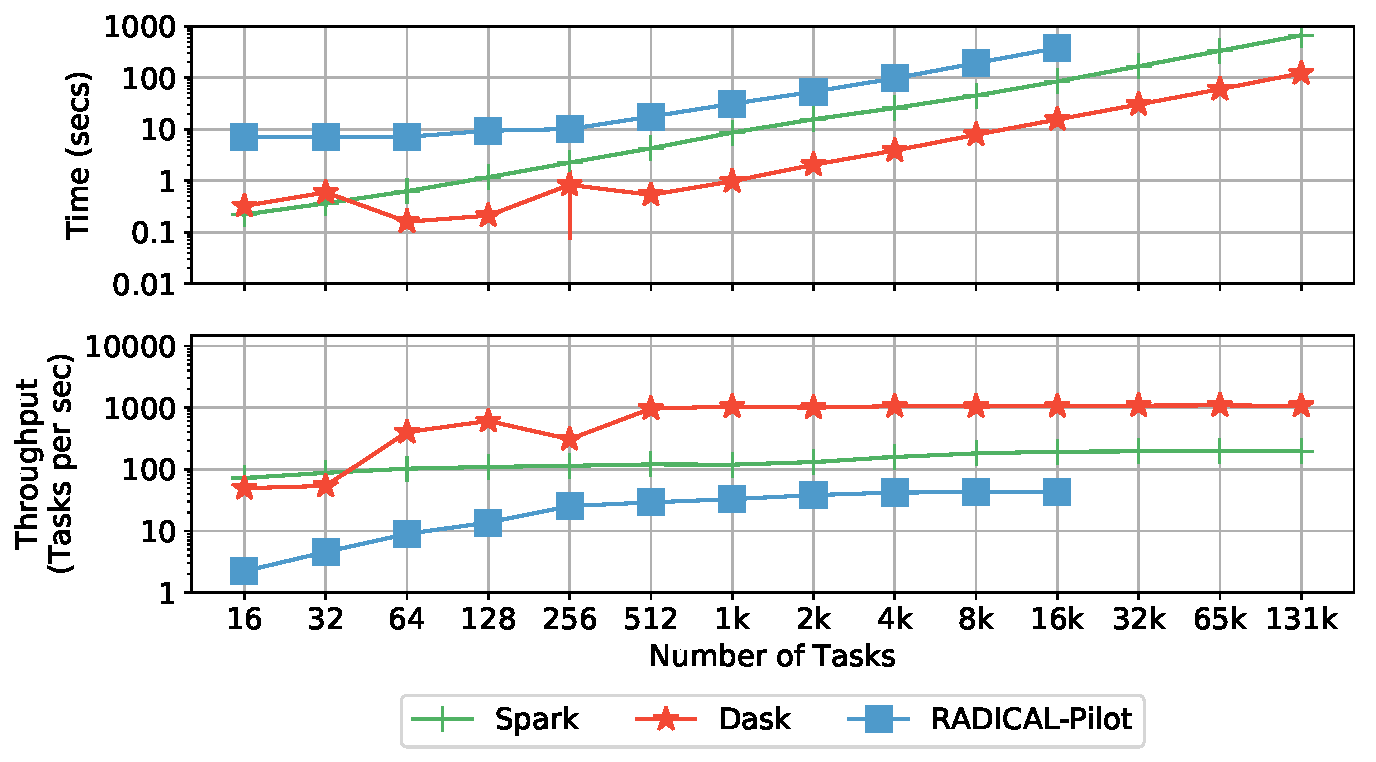
\includegraphics[width=.95\textwidth]{figures/data_analytics_hpc/task_par/dask_spark_rp_wrangler.pdf}
    \caption{Total time to completion and task throughput by framework on a single node for an increasing number of tasks.}
    %\caption{\textbf{Task Throughput by Framework (Single Node):} 
    %    Time/Throughput executing a given number of zero-workload tasks on Wrangler.
    %    Dask performs best; Dask and Spark have very small delays for few tasks.
    %    RADICAL~-Pilot offers the smallest throughput.}
    \label{fig:dask_spark_rp_wrangler}
\end{figure}

Figure~\ref{fig:dask_spark_rp_wrangler} shows the total time to completion and task throughput.
Dask needed the least time to schedule and execute the assigned tasks, followed by Spark and RADICAL~-Pilot.
Dask and Spark quickly reach their maximum throughput, which is sustained as the number of tasks increased.
RADICAL~-Pilot showed the worst throughput and scalability mainly due to some architectural limitations.
It relies on a MongoDB to communicate between Client and Agent, as well as several components that allow RADICAL~-Pilot to move data and introduce delays in the execution of the tasks.
Thus, we were not able to scale RADICAL~-Pilot to 32k or more tasks.

\begin{figure}[t]
    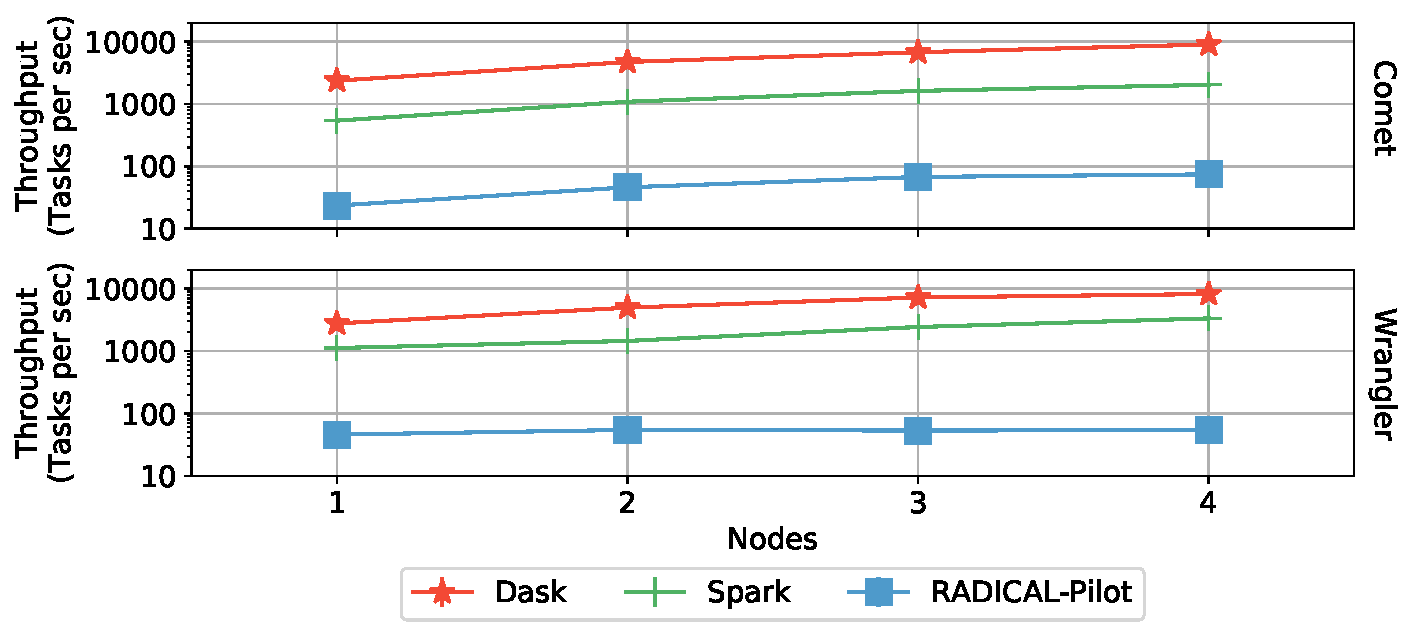
\includegraphics[width=.95\textwidth]{figures/data_analytics_hpc/task_par/daskVSsparkVSRpThroughput.pdf}
    \caption{Task throughput by framewrork for $100k$ tasks on different number of nodes.}
    %\caption{\textbf{Task Throughput by Framework (Multiple Nodes):}
    %    Task throughput for $100k$ zero-workload tasks on different numbers of nodes for each framework. 
    %    Dask has the largest throughput, followed by Spark and RADICAL~-Pilot.}
    \label{fig:RP_Dask_Spark_throughput}
\end{figure}

Figure~\ref{fig:RP_Dask_Spark_throughput} illustrates the throughput when scaling to multiple nodes measured by submitting $100k$ tasks.
Dask's throughput on both resources increases almost linearly to the number of nodes.
Spark's throughput is an order of magnitude lower than Dask's.
RADICAL~-Pilot's throughput plateaus at below $100 task/sec$.
Wrangler and Comet show a comparable performance with Comet slightly outperforming Wrangler.

%\subsubsection*{Suitability for MDAnalysis Algorithms}
%Trajectory analysis methods are often embarrassingly parallel.
%So, they are ideally suited for task management and MapReduce APIs.
%PSA-like methods typically require a single pass over the data and return a set of values that correspond to a relationship between frames or trajectories.
%They can be expressed as a bag of tasks using a task management API or a map-only application in a MapReduce-style API.

%Leaflet Finder is more complex and requires two stages:
%\begin{inparaenum}[a)]
%    \item the edge discovery stage, and
%    \item the connected components stage.
%\end{inparaenum}
%It is possible to implement Leaflet Finder with a simple task-management API, although the MapReduce programming model allows more efficient implementation with a \texttt{map} for computing and filtering distances and a \texttt{reduce} for finding the components.
%The shuffling required between map and reduce is medium as the number of edges is a fraction of the input data.

\section{Task-Parallel MD Trajectory Data Analysis: Implementation \& Characterization}
\label{impl_exp}
In this section, we characterize the performance of RADICAL~-Pilot, Spark and Dask compared to MPI4py.
In section~\ref{sec:framework_eval} we evaluate the task throughput using a synthetic workload.
In sections~\ref{sec:psa} and~\ref{sec:leaflet} we evaluate the performance of two algorithms from MDAnalysis: PSA and Leaflet Finder using different real-world datasets.
We investigate: 
\begin{inparaenum}[1)]
    \item which capabilities and abstractions of the frameworks are needed to efficiently express these algorithms,
    \item what architectural approaches can be used to implement these algorithms with these frameworks, and
    \item the performance trade-offs of these frameworks.
\end{inparaenum}

The experiments were executed on the XSEDE Supercomputers: Comet and Wrangler.
SDSC Comet is a 2.7 PFlop/s cluster with 24\, Haswell cores/node and 128\,GB memory/node (6,400 nodes).
TACC Wrangler has 24\, Haswell hyper-threading enabled cores/node and 128\,GB memory/node (120 nodes).
Experiments were carried using RADICAL~-Pilot and Pilot-Spark (as discusses on \S~\ref{sec:pilot-data-hadoop}) extension, which allows to efficiently manage Spark on HPC resources through a common resource management API.
We utilize a set of custom scripts to start the Dask cluster.
We used RADICAL~-Pilot 0.46.3, Spark 2.2.0, Dask 0.14.1 and Distributed 1.16.3.
The data presented are means over multiple runs; error bars represent the standard deviation of the sample.
We employed up to $10$ nodes in Comet and Wrangler. 

\subsection{Path Similarity Analysis: Hausdorff Distance}
\label{sec:psa}
The PSA algorithm is embarrassingly parallel and can be implemented using simple task-level parallelism or a map only MapReduce application.
The input data, i.\,e. a set of trajectory files, is equally distributed over the cores, generating one task per core.
Each task reads its respective input files in parallel, executes and writes the result to a file.

For RADICAL~-Pilot we define a Compute~-Unit for each task and execute them using a Pilot-Job. 
For Spark, we create an RDD with one partition per task.
The tasks are executed in a \texttt{map} function.
In Dask, the tasks are defined as \texttt{delayed} functions.
In MPI, each task is executed by a process.

The experiments were executed on Comet and Wrangler. 
The dataset used consists of three different atom count trajectories: 
\begin{inparaenum}[1)]
    \item small ($3341$ atoms/frame), 
    \item medium ($6682$ atoms/frame) and 
    \item large ($13364$ atoms/frame).
\end{inparaenum}
We used $102$ frames, and $128$ and $256$ trajectories of each size.

Figure~\ref{fig:HausdorffWrangler} shows the runtime for 128 and 256 trajectories on Wrangler.
Figure~\ref{fig:comet_wrangler_haus} compares the execution times on Comet and Wrangler for $128$ large trajectories.
We see that the frameworks have similar performance on both systems.
Furthermore, we see that Wrangler gives smaller speedup than Comet.
Although, we used the same number of cores, we see that utilizing half the nodes due to hyperthreading results to smaller speedup.

\begin{figure}[t]
    \centering
    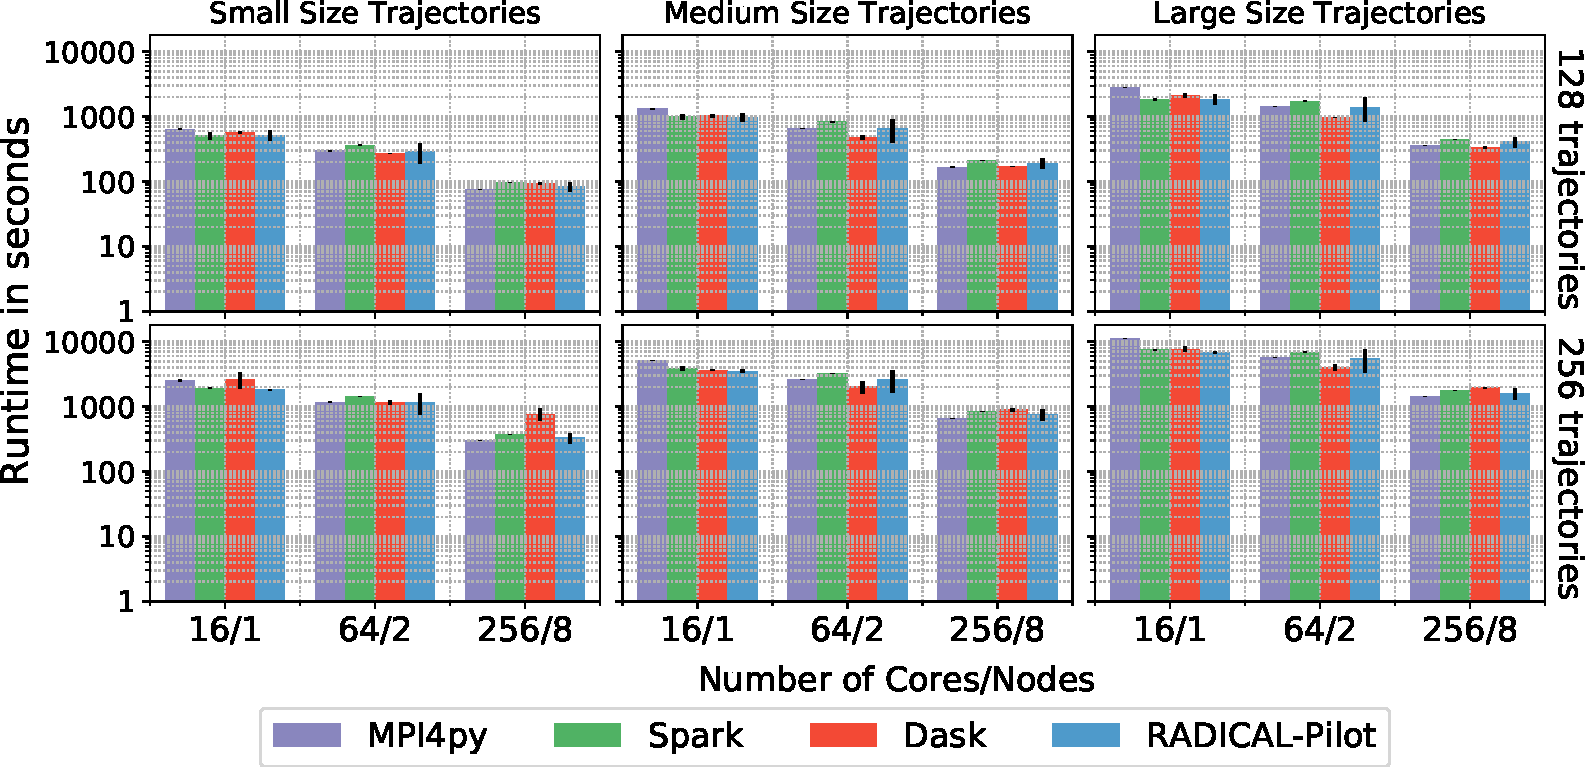
\includegraphics[width=0.95\textwidth]{figures/data_analytics_hpc/task_par/HausdorffSingleFig.pdf}
    \caption{Time to completion of Hausdorff Distance on Wrangler using RADICAL~-Pilot, Spark and Dask over different number of cores, trajectory sizes, and number of trajectories.}
%    \caption{\textbf{Hausdorff Distance on Wrangler using RADICAL~-Pilot, Spark and Dask:}
%            Runtimes over different number of cores, trajectory sizes, and number of trajectories.
%            All frameworks scaled by a factor of 6 from 16 to 256 cores.}
            \label{fig:HausdorffWrangler}
\end{figure}

\begin{figure}[t]
    \centering
    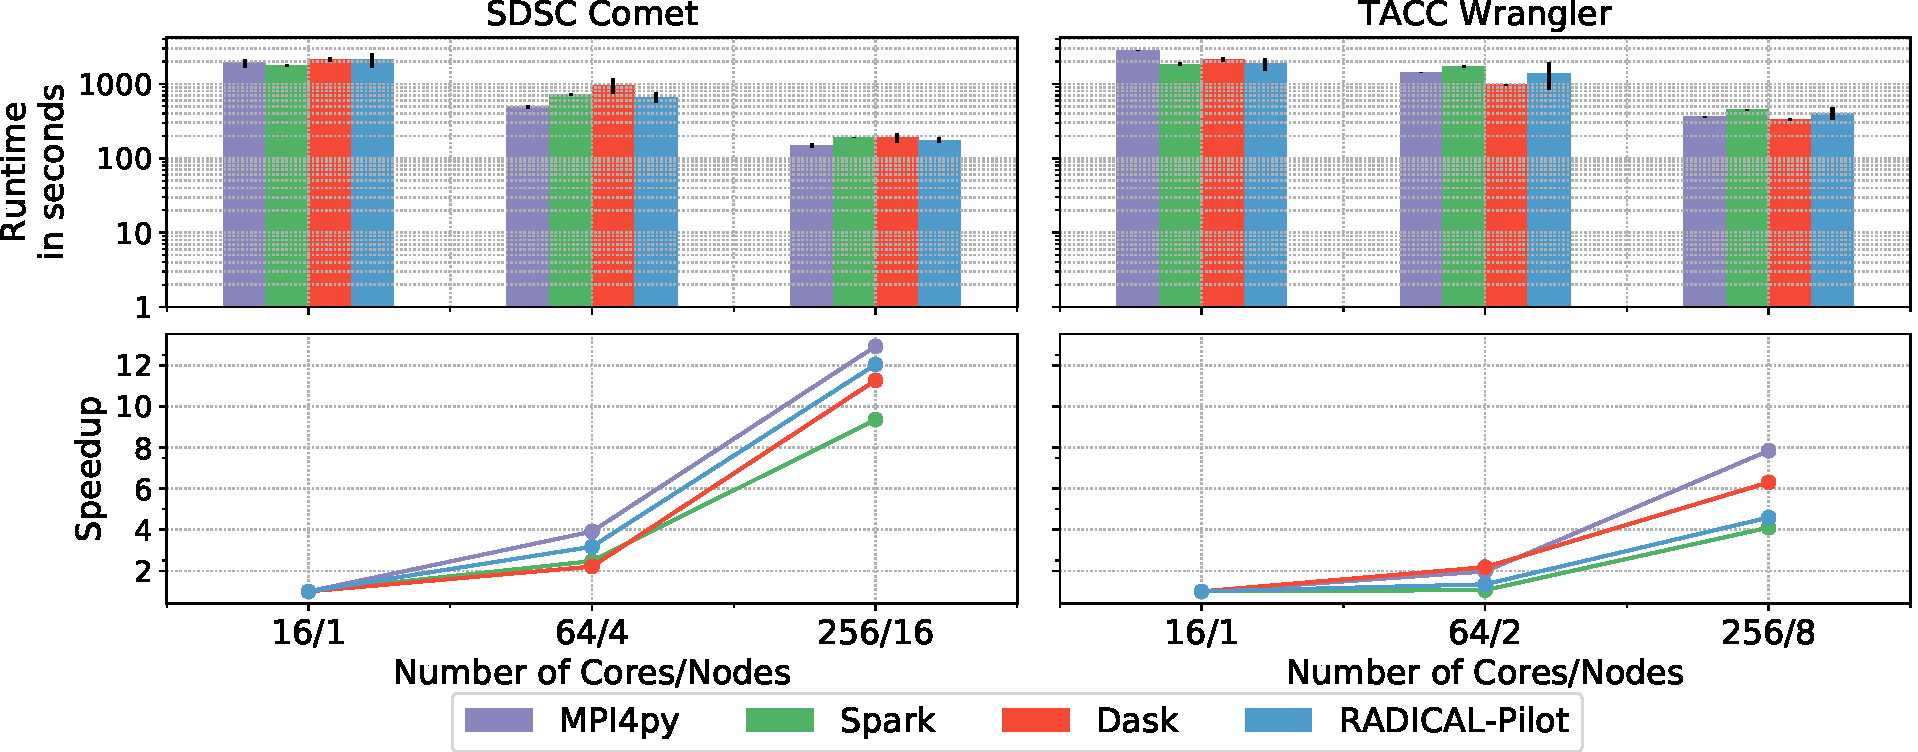
\includegraphics[width=.95\textwidth]{figures/data_analytics_hpc/task_par/comet_wrangler_haus.pdf}
    \caption{Time to completion and speedup of Hausdorff Distance execution on Comet and Wrangler for 128 large trajectories.} 
    \label{fig:comet_wrangler_haus}
\end{figure}

MPI4py, RADICAL~-Pilot, Spark and Dask have similar performance when used to execute embarrassingly parallel algorithms.
All frameworks achieved similar speedups as the number of cores increased, scaling by a factor of 6 from 16 to 256 cores, which are lower than MPI4py.
Although, the frameworks' overheads are comparably low in relation to the overall runtime, they were significant to impact their speedup.
RADICAL~-Pilot's large deviation is due to sensitivity to communication delays with the database.
In summary, all three frameworks provide appropriate abstractions and runtime performance, compared to MPI, for embarrassingly parallel algorithms. 
In this case aspects such as programmability and integrate-ability are more important considerations,e.\,g., both RADICAL~-Pilot and Dask are native Python frameworks making the integration with python native frameworks easier and more efficient than with other frameworks, which are based on other languages.

%\begin{figure}[ht]
%    \centering
%    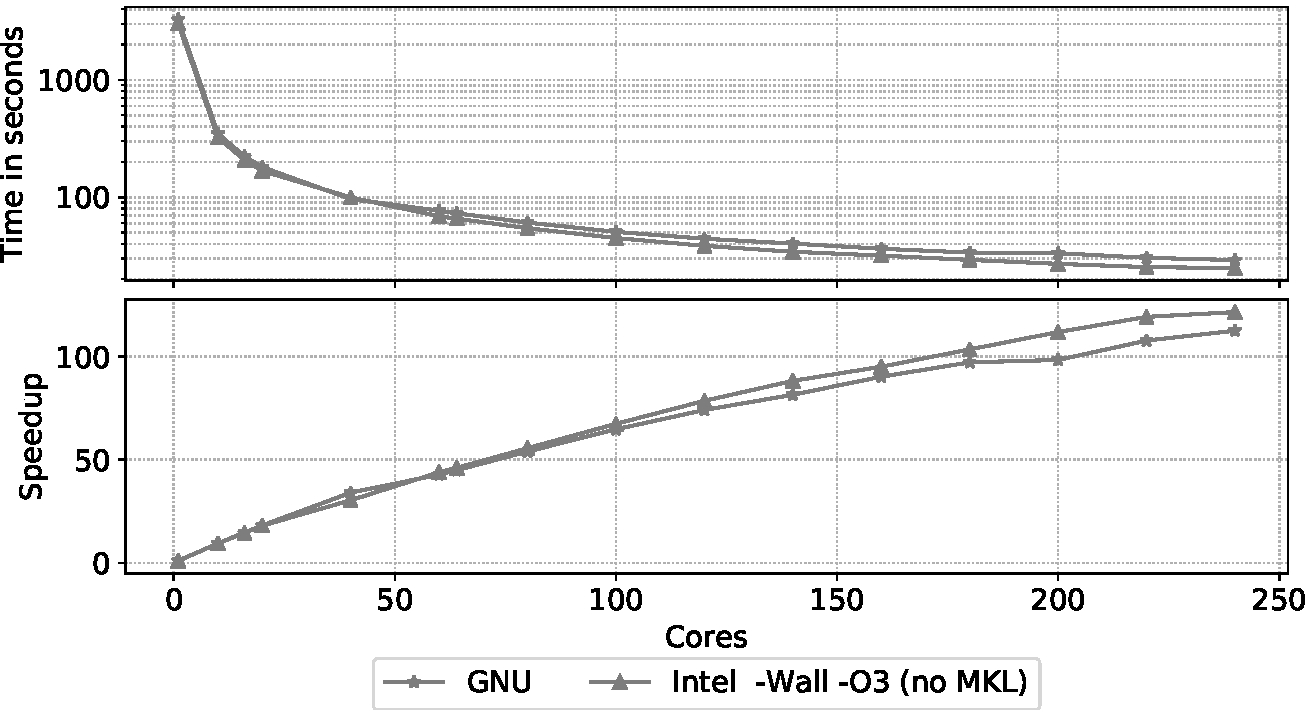
\includegraphics[width=.95\textwidth]{figures/data_analytics_hpc/task_par/cpptrajHausdorff.pdf}
%    \caption{\label{fig:cpptraj_resutls}\textbf{Hausdorff Distance using CPPTraj:}
%    Runtimes and Speedup over different number of cores.} 
%\end{figure}

%CPPTraj~\cite{roe2018parallelization} provides an optimized C++ implementation of the 2D-RMSD, which is Algorithm~\ref{alg:hausdorff} with no $\min-\max$ operations.
%The 2D-RMSD between trajectories was executed in parallel.
%The results were gathered and the Hausdorff distance was calculated.
%CPPTraj~\cite{roe2018parallelization} was compiled with GNU C++ compiler and no optimizations, and with Intel's compiler O3 optimization enabled.
%An experiment was run with 20-core Haswell nodes and 128 small trajectories; number of cores ranging from 1 up to 240.
%Figure~\ref{fig:cpptraj_resutls} shows the runtimes and speedup.
%MPI C++ provides lower execution times.
%However, we are interested in scalable solutions, that may offer worse performance in absolute numbers, but allows easier integration, i.e., less lines of code, and/or less engineering time.

\subsection{Leaflet Finder}
\label{sec:leaflet}
\begin{table*}[t]
    \centering
    \begin{tabular}{@{}p{2cm}|p{2.8cm}p{2.8cm}p{2.8cm}p{2.8cm}@{}}
        \toprule
        &
        \textbf{Broadcast and 1-D} (Approach 1) &
        \textbf{Task API and 2-D} (Approach 2) &
        \textbf{Parallel Connected Components} (Approach 3) &
        \textbf{Tree-Search} (Approach 4)\\
        \midrule
        % row 1
        Data Partitioning  & 
        1D  & 
        2D & 
        2D & 
        2D\\
        % row 2
        Map & 
        Edge Discovery via Pairwise Distance &
        Edge Discovery via Pairwise Distance &
        Edge Discovery via Pairwise Distance and Partial Connected Components & 
        Edge Discovery via Tree-based Algorithm and Partial Connected Components\\
        % row 3
        Shuffle &
        Edge List ($O(E)$) &
        Edge List ($O(E)$) &
        Partial Connected components ($O(n)$) &
        Partial Connected components ($O(n)$)\\
        % row 4
        Reduce   &
        Connect Components  &
        Connected Components &
        Joined Connected Components &
        Joined Connected Components\\
        \bottomrule
    \end{tabular}
    \caption{MapReduce Operations used by Leaflet Finder\label{tab:app_operators}}
\end{table*}

\begin{figure*}[t]
    \centering
    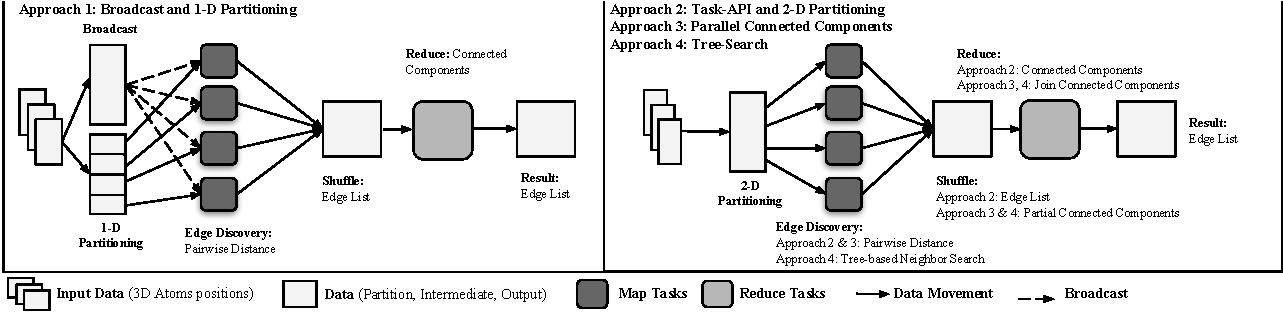
\includegraphics[width=.98\textwidth]{figures/data_analytics_hpc/task_par/lf_approaches.pdf}
    \caption{Architectural approaches for implementing the Leaflet finder algorithm\label{fig:lf_approaches}} 
\end{figure*}

We developed four different approaches for implementing the Leaflet Finder algorithm using RADICAL~-Pilot, Spark, Dask, and MPI4py (see Fig~\ref{fig:lf_approaches} and Table~\ref{tab:app_operators}):
\begin{enumerate}[1)]
    \item \textbf{Broadcast and 1-D Partitioning:}
    The physical system is broadcast and partitioned through a data abstraction.
    Use of RDD API (broadcast), Dask Bag API (scatter), and MPI Bcast to distribute data to all nodes.
    A \texttt{map} function calculates the edge list using \texttt{cdist} from SciPy~\cite{scipy} -- realized as a loop for MPI.
    The list is collected to the master process (gathered to rank 0) and the connected components are calculated.\label{en:1}
    \item \textbf{Task API and 2-D Partitioning:}
    Data management is done without using the data-parallel API.
    The framework is used for task scheduling.
    Data are pre-partitioned in 2-D partitions and passed to a \texttt{map} function that calculates the edge list using \texttt{cdist}-- realized as a loop for MPI.
    The list is collected (gathered to rank 0) and the connected components are calculated.\label{en:2}
    \item \textbf{Parallel Connected Components:}
    Data are managed as in approach~\ref{en:2}.
    Each \texttt{map} task performs edge list and connected components computations.
    The reduce phase joins the calculated components into one, when there is at least one common node.\label{en:3}
    \item \textbf{Tree-based Nearest Neighbor and Parallel-Connected Components (Tree-Search):}
    This approach is different to approach~\ref{en:3} only on the way edge discovery in the \texttt{map} phase is implemented.
    A tree containing all atoms is created which is then used to query for adjacent atoms.\label{en:4}
\end{enumerate}

We use four physical systems with $131k$, $262k$, $524k$, and $4M$ atoms with $896k$, $1.75M$, $3.52M$, and $44.6M$ edges in their graphs.
Experimentation was conducted on Wrangler where we utilized up to 256 cores.
Data partitioning results into $1024$ partitions for each approach, thus $1024$ \texttt{map} tasks.
Due to memory limitations from using \texttt{cdist} -- uses double precision floating point -- Approach \ref{en:3} data partitioning of the $4M$ atom dataset resulted to $42k$ tasks for both Spark and MPI4py.

Figure \ref{fig:All4approachesNoRp} shows the runtimes for all datasets for Spark, Dask and MPI4py.
RADICAL~-Pilot's performance is illustrated in Figure~\ref{fig:rpLF}.
We continue by analyzing the performance of each architectural approach and used framework in detail.

\begin{figure}[t]
    \begin{subfigure}{.95\textwidth}
        \centering
        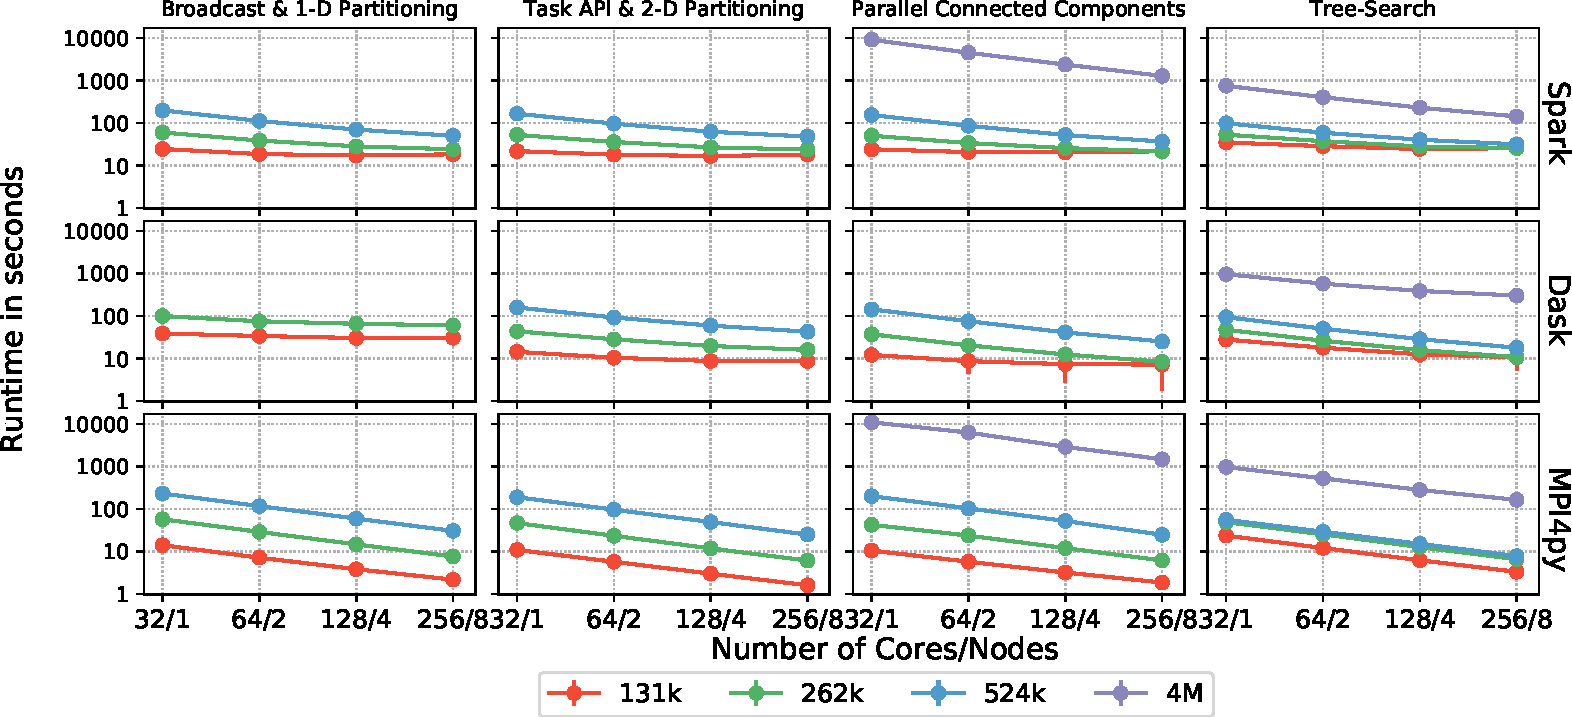
\includegraphics[width=1\linewidth]{figures/data_analytics_hpc/task_par/All4approachesWith4M_logscaleline.pdf}
    \end{subfigure}\\
    \begin{subfigure}{.95\textwidth}
        \centering
        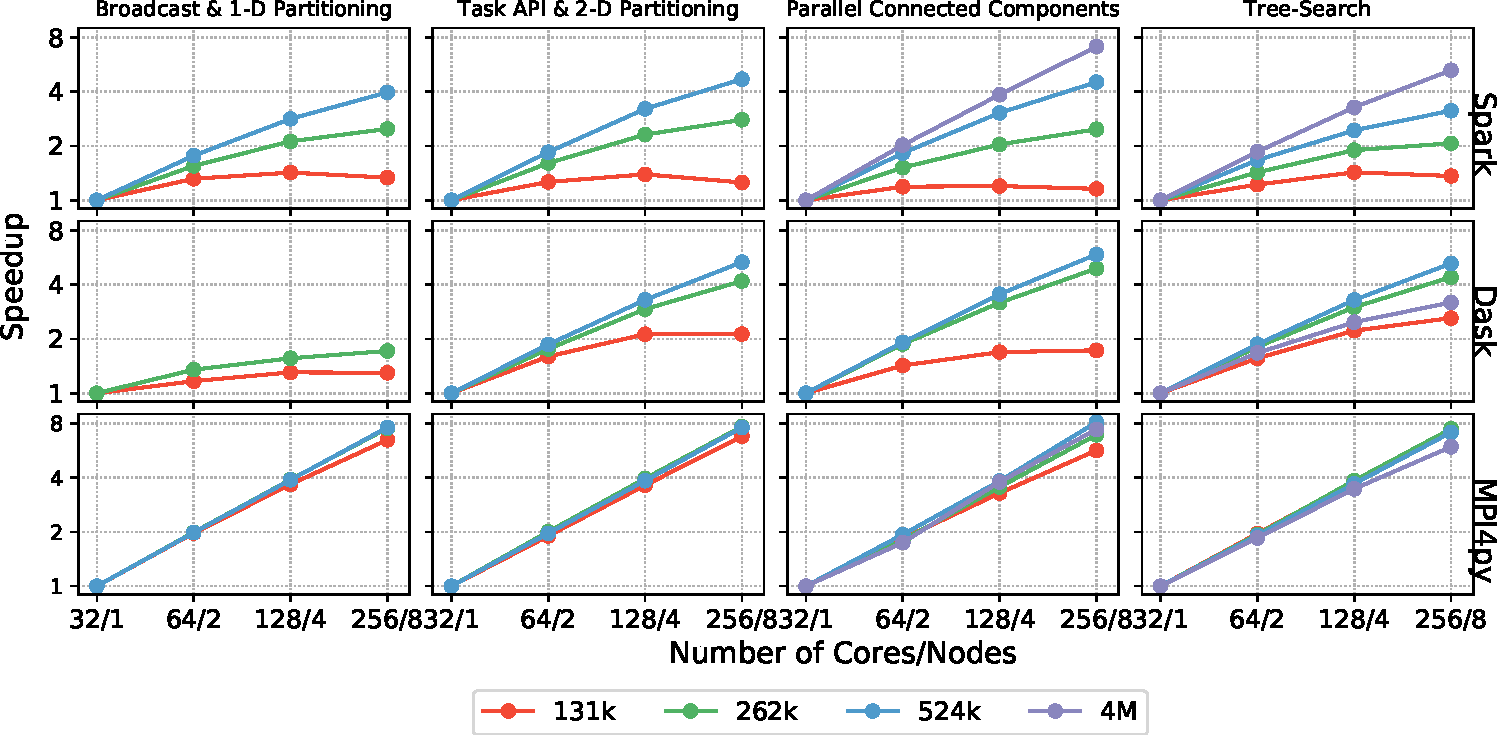
\includegraphics[width=.95\linewidth]{figures/data_analytics_hpc/task_par/All4approachesWith4MSpeedup.pdf}
    \end{subfigure}
    \caption{Leaflet Finder Performance of Different Architectural Approaches for Spark \& Dask.
            Runtimes and Speedups for different system sizes over different number of cores for all approaches and frameworks.}
    \label{fig:All4approachesNoRp}
\end{figure}

%%%%%%%%%%%%%%% APPROACH 1 %%%%%%%%%%%%%%%%%%

\begin{figure}[t]
    \centering
    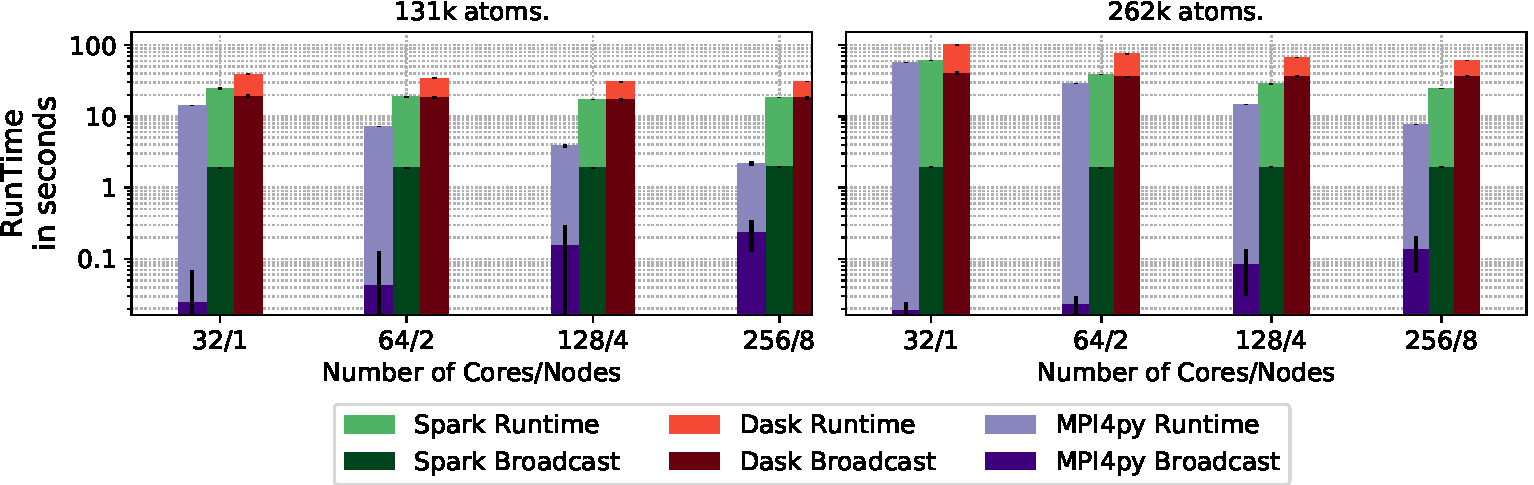
\includegraphics[width=.95\textwidth]{figures/data_analytics_hpc/task_par/spark_dask_lf_approach1.pdf}
    \caption{Broadcast and 1-D Partitioned Leaflet Finder (Approach 1).
    Runtime for multiple system sizes on different number of cores for Spark, Dask and MPI4py.}
    \label{fig:WranglerLeafLetFinderApp1}
\end{figure}

\subsubsection*{Broadcast and 1-D Partitioning}
Approach 1 utilizes a broadcast to distribute the data to all nodes, which is supported by Spark, Dask and MPI.
All nodes maintain a complete copy of the dataset.
Each \texttt{map} task computes the pairwise distance on its partition.
We use 1-D partitioning.
Figure~\ref{fig:WranglerLeafLetFinderApp1} shows the detailed results: as expected the usage of a broadcast has severe limitations for Spark and Dask.
MPI broadcast is a fraction of the overall execution time and significantly smaller than Spark and Dask.
MPI's broadcast times increase linearly as the number of processes increases, while Spark's and Dask's remain relatively constant for each dataset, due to more elaborate broadcast algorithms compared to MPI.
Broadcast times are about $3\%$ -- $15\%$ of the edge discovery time for Spark, $40\%$ -- $65\%$ for Dask, and $<1\%$ -- $10\%$ for MPI4py.
Spark offers a more efficient communication subsystem compared to Dask.
In addition, Dask broadcast partitions the dataset to a list where each element represents a value from the initial dataset.
This did not allow broadcasting the $524k$ atom dataset.
Nevertheless, the limited scalability of this approach due to transmitting the entire dataset renders it only usable for small datasets.
It shows the worst performance and scaling of all approaches for Spark, Dask and MPI4py.

Furthermore, this approach only scales up to $262k$ atoms for Dask, and $524k$ atoms for Spark and MPI4py on Wrangler.
Spark's performance is comparable to MPI4py for the $262k$, and $524k$ datasets.
It also shows better performance for the smallest core count in the $524k$ case.
Dask is at least two times slower than our MPI implementation.

%%%%%%%%%%%%%%% APPROACH 2 %%%%%%%%%%%%%%%%%%


\begin{figure}[t]
    \centering
    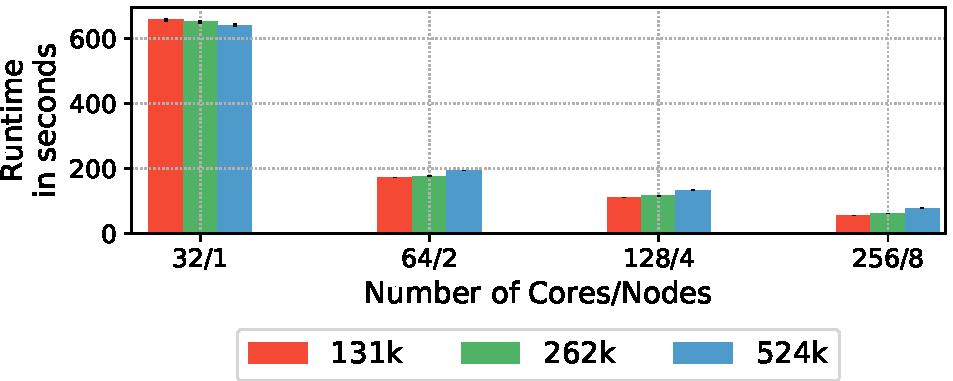
\includegraphics[width=.95\textwidth]{figures/data_analytics_hpc/task_par/rpLF.pdf}
    \caption{RADICAL~-Pilot Task API and 2-D Partitioned Leaflet Finder (Approach 2).
    Runtime for multiple system sizes over different number of cores.}
    %Overheads dominate since execution times are similar despite the system size.}
    \label{fig:rpLF}
\end{figure}

\subsubsection*{Task-API and 2-D Partitioning}
Approach~\ref{en:2} tries to overcome the limitations of approach 1, especially broadcasting and 1-D partitioning.
A 2-D block partitioning is essential, as it evenly distributes the compute and more efficiently utilizes the available memory.
2-D partitioning is not well supported by Spark and Dask.
Spark's RDDs are optimized for data-parallel applications with 1-D partitioning.
While Dask's array supports 2-D block partitioning, it was not used for this implementation.
We return the adjacency list of the graph instead of an array to fully use the capabilities of the abstraction.
Thus, each task works on a 2-D pre-partitioned part of the input data.

Figure~\ref{fig:All4approachesNoRp} shows the runtimes of approach~\ref{en:2} for Spark, Dask, MPI4py and Figure~\ref{fig:rpLF} for RADICAL~-Pilot.
As expected this approach overcomes the limitations of approach 1 and can easily scale to larger datasets (e.\,g., $524k$ atoms) while improving the overall runtime.
Dask's execution time was smaller by at least a factor of two.
However, we were not able to scale this implementation to the 4M dataset, due to memory requirements of \texttt{cdist}.
For RADICAL~-Pilot we observed significant task management overheads (see also section~\ref{sec:framework_eval}).
This is a limitation of RADICAL~-Pilot with respect to managing large numbers of tasks.
This is particularly visible when the scenario was run on a single node with 32 cores.
As more resources become available, i.e. more than 64 cores, the performance improves dramatically.

Furthermore, Spark and Dask did not scale as well as MPI, which achieved linear speedups of $\sim8$ when using $256$ cores.
Spark and Dask achieved maximum speedups of $4.5$ and $\sim5$ respectively.
Despite this fact, both frameworks had similar performance on $32$ cores for the $262k$ and $524k$ datasets.

%%%%%%%%%%%%%% Approach 3 %%%%%%%%%%%%%%%%%%%%%%%

\subsubsection*{Parallel Connected Components}
Communication between the edge discovery and connected components stages is another important aspect.
The edge discovery phase output for the $524k$ atoms dataset is $\approx$ $100\,\textup{MB}$.
To reduce the amount of data that need to be shuffled, we refined the algorithm to compute the graph components on the partial dataset in the \texttt{map} phase.
The partial components are then merged in a \texttt{reduce} phase.
This reduces the amount of shuffle data by more than $50\%$ (e.\,g., to $12\textup{MB}$ for Spark and $48\textup{MB}$ for Dask).
Figure~\ref{fig:All4approachesNoRp} shows the improvements in runtime, by $\sim20\%$ for Spark and Dask, but not MPI4py.
Further, we were able to run very large datasets, such as the 4M dataset, using this architectural approach using Spark and MPI4py.
Dask was restarting its worker processes because their memory utilization was reaching $95\%$.

Spark, and Dask have comparable performance with MPI on 32 cores, which utilizes a single node on Wrangler.
However, the MPI4py implementation scales almost linearly for all datasets, Spark and Dask cannot, reaching a maximum of $\sim5$ for the three smaller datasets.
In addition, Spark is able to scale almost linearly for the $4M$ atoms dataset providing comparable performance to MPI4py.

%%%%%%%%%%%%%% Approach 4 %%%%%%%%%%%%%%%%%%%%%%%

\subsubsection*{Tree-Search}
A bottleneck of approaches~\ref{en:1},~\ref{en:2} and~\ref{en:3} is the edge 
discovery via the naive calculation of the distances between all pairs of atoms. 
In approach~\ref{en:4}, we replace the pairwise distance function with a tree-based, 
nearest neighbor search algorithm, in particular BallTree~\cite{omohundro89five}. 
The algorithm: 
\begin{inparaenum}
    \item constructs of a tree, and
    \item queries for neighboring atoms.
\end{inparaenum}

Using tree-search, the computational complexity can be reduced from $n^2$ to $log$. 
We use a BallTree as offered by Scikit-Learn~\cite{scikit-nearest} for our implementation.

Figure \ref{fig:All4approachesNoRp} illustrates the performance of the implementation.
For small datasets, i.\,e., $131k$ and $262k$ atoms, approach~\ref{en:3} is faster than the tree-based approach, since the number of points is too small.
For the large datasets, the tree approach is faster.
In addition, the tree has a smaller memory footprint than \texttt{cdist}.
This allowed to scale to larger problems, e.\,g., a $4M$ atoms and $44.6M$ edges dataset without changing the total number of tasks.

Dask shows better scaling than Spark for $131k$, $262k$, and $524k$ atoms.
This is not true for $4M$ atoms, indicating that Dask's communication layer is not able to scale as well as Spark's.
Spark shows similar performance with MPI4py for the largest dataset due to minimal shuffle traffic.
Thus, MPI's efficient communication does not become relevant.

\section{Task-Parallel Framework Selection Conceptual Model and Discussion}
In this section we provide a conceptual model that allows application developers to carefully select a framework according to their requirements (e.\,g., compute and I/O).
It is important to understand both the properties of the application and Big Data frameworks.
Table~\ref{tab:framework} illustrates the criteria of this conceptual model and ranks the three frameworks.

\begin{table}[t]
    \centering
    \begin{tabular}{@{}cccc@{}}
        \toprule
        &\textbf{RADICAL~-Pilot}     &\textbf{Spark} &\textbf{Dask}\\
        \multicolumn{4}{l}{\textbf{Task Management}} \\
        \midrule
        Low Latency   &- &o &+\\
        Throughput    &- &+ &++\\
        MPI/HPC Tasks &+ &o &o\\
        Task API   &+ &o &++\\
        Large Number of Tasks   &-- &++ &++\\\hline
        \multicolumn{4}{l}{\textbf{Application Characteristics}}\\\midrule
        Python/native Code &++ &o &+\\
        Java               &o &++ &o\\
        Higher-Level Abstraction &- &++ &+\\
        Shuffle                  &- &++ &+\\
        Broadcast                &- &++ &+\\
        Caching                  &- &++ &o\\
        \bottomrule
    \end{tabular}
    \caption{Task-parallel framework selection decision methodology: Criteria and Ranking for Framework Selection. -~: Unsupported or low performance
        +~: Supported, ++~: Major Support, and o~:Minor support.\label{tab:framework}}
\end{table}
%  application perspective

\subsubsection*{Application Perspective}
We showed that we can implement MD trajectory data analysis applications using all three frameworks, as well as MPI4py.
Implementation aspects, such as computational complexity, and shuffled data size influence the performance greatly.
For embarrassingly parallel applications with coarse grained tasks, such as PSA, the choice of the framework does not significantly influence performance (Figures~\ref{fig:HausdorffWrangler} and~\ref{fig:comet_wrangler_haus}).
In addition, the performance difference against MPI4py was not significant (Figures~\ref{fig:HausdorffWrangler} and~\ref{fig:comet_wrangler_haus}).
Thus, aspects, such as programmability and integrate-ability, become more important.

For fine-grained data parallelism, a Big Data framework, such as Spark and Dask, clearly outperforms RADICAL~-Pilot (Figures~\ref{fig:All4approachesNoRp},~\ref{fig:rpLF}).
If coupling is introduced, i.\,e. task communication is required (e.\,g., reduce), using Spark becomes advantageous (Approaches~\ref{en:3} \& \ref{en:4}). 
PI4py outperformed Dask, and Spark, despite both frameworks scaling for the larger datasets.
Especially Spark was able to provide linear speedup for approach~\ref{en:3} of Leaflet Finder (Figure~\ref{fig:All4approachesNoRp}).
Integrating with frameworks that provide higher level abstractions provides scalable solutions for more complex algorithms.
However, integrating Spark with other tools needs to be carefully considered.
The integration of Python tools, e.\,g. MDAnalysis, often causes overheads due to the frequent need for serialization and copying data between the Python and Java space.

Dask had the smallest learning curve of all three frameworks.
As a result, it allows for faster prototyping compared to RADICAL~-Pilot and Spark.
RADICAL~-Pilot's learning curve is more steep, but is more versatile than Dask and Spark, by offering the lowest level abstraction. 
Spark had the slowest learning curve.
It required tuning to get the number of tasks correctly, as well as argument passing to map and reduce functions.

\subsubsection*{Framework Perspective}
RADICAL~-Pilot is well suited for HPC applications, e.\,g., ensembles (up to $50k$ tasks) of parallel MPI applications, as shown in Ref.~\cite{merzky2018design,merzky2019using}.
It has limited scalability when supporting large numbers of short-running tasks, as often found in data-intensive workloads.
The file staging implementation of RADICAL~-Pilot is not suitable for supporting the data exchange patterns, i.e. shuffling, required for these applications.
However, executing MPI and Spark applications alongside on the same resource makes RADICAL~-Pilot particularly suitable when different programming models need to be combined.

% framework perspective
Dask provides a highly flexible, low-latency task management and excellent support for parallelizing Python libraries.
We established that Dask has higher throughput (Figures~\ref{fig:dask_spark_rp_wrangler} and~\ref{fig:RP_Dask_Spark_throughput}).
However, Spark provides better speedups for the largest datasets compared to Dask (Figure ~\ref{fig:All4approachesNoRp}).
Dask's broadcast (Leaflet Finder approach~\ref{en:1}) and shuffle (Leaflet Finder approaches~\ref{en:2}-~\ref{en:4}) performance is worse for larger problems compared to Spark.
Thus, Dask's communication layer shows some weaknesses that are particularly visible during broadcast and shuffle.
Spark needs to be particularly considered for shuffle-intensive applications.
Its in-memory caching mechanism is particularly suited for iterative algorithms that maintain a static set of data in-memory and conduct multiple passes on that set.


% ---------------------------------------------------------
% CHAPTER 4
% ---------------------------------------------------------
\chapter{Evaluating Middleware for Task-Parallel Data Analytics on HPC Platforms}
\label{ch:designs}
% !TEX root = main.tex
\label{ch:designs}

This far, we have discussed how to efficiently and scalably support the execution of MapReduce workflows, as part of a computational campaign, on High Performance Computing (HPC) resources.
There are, though, computational campaigns whose workflows do not necessarily conform to the MapReduce abstraction.
The tasks of such workflows can be heterogeneous, implementing a diverse set of functionalities that are compute-intensive.
As a consequence, data-parallel frameworks, like Spark and Dask may not be the most suitable choice for their execution.
From a middleware perspective, the design and architectural space is large and the lack of performance analysis makes it difficult to select among equivalent implementations.

From a design perspective, a promising approach is isolating tasks from execution management.
Tasks are assumed to be self-contained programs which are executed in the operating system (OS) environment of HPC compute nodes.
Compared to approaches in which tasks are functions or methods, a program-based approach offers several benefits as, for example, simplified implementation of execution management, support of general purpose programming models, and separate programming of management and domain-specific functionalities.
Nonetheless, program-based designs also impose performance limitations, including OS-mediated intertask communication and task spawning overheads, as programs execute as OS processes and do not share a memory space.

Due to their performance limitations, program-based designs of computing frameworks are best suited to execute compute-intense workflows in which each task requires a certain amount of parallelism and runs from several minutes to hours.
The emergence of workflows that require heterogeneous, compute-intense tasks to process large amount of data is pushing the boundaries of program-based designs, especially when scale requirements suggest the use of modern HPC infrastructures with large number of CPUs/GPUs and dedicated data facilities.

We use a paradigmatic use case workflow from the polar science domain to evaluate three alternative task-based designs, and experimentally characterize and compare their performance.
Our use case requires us to analyze satellite images of Antarctica to detect pack-ice seals taken across a whole calendar year.
The resulting dataset consists of $3,097$ images for a total of $\approx4$~TB.
The use case requires us to repeatedly process these images, running both CPUs and GPUs code that exchange several GB of data.
The first design uses a pipeline to independently process each image, while the second and third designs use the same pipeline to process a series of images with differences in how images are bound to available compute nodes.

The chapter is organized as follows.
Section~\ref{sec:ucase} presents the use case and discusses it computational requirements as well as its task-based workflow.
In \S~\ref{sec:design}, we discuss the three architecturally equivalent design to support task-based workflows.
 \S\ref{sec:des_experiments} presents a performance evaluation of the designs and discusses the lessons learned.
 
 \section{Related Work}
Several tools and frameworks are available for image analysis based on diverse designs and programming paradigms, and implemented for specific resources.
Numerous image analytics frameworks for medical, astronomical, and other domain specific imagery provide MapReduce implementations.
MaReIA~\cite{vo2018mareia}, built for medical image analysis, is based on Hadoop and Spark~\cite{zaharia2010spark}.
Kira~\cite{zhang2016kira}, built for astronomical image analysis, is also built on top of Spark and pySpark, allowing users to define custom analysis applications.
Further, Ref.~\cite{yan2014large} proposes a Hadoop-based cloud Platform as a Service, utilizing Hadoop's streaming capabilities to reduce filesystem reads and writes.
These frameworks support clouds and/or commodity clusters for execution.
 
BIGS~\cite{ramos2012bigs} is a framework for image processing and analysis.
BIGS is based on the master-worker model and supports heterogeneous resources, such as clouds, grids and clusters.
The user is responsible to define the input, processing pipeline, and launch BIGS workers.
BIGS utilizes a database to perform data transfers between workers.
In addition, BIGS offers a diverse set of APIs for developers.
BIGS approach is very close to Design 1 we described in~\S\ref{des1}.

Image analysis libraries, frameworks and applications have been proposed for HPC resources.
PIMA(GE)\textsuperscript{2} Library~\cite{galizia2015mpicuda} provides a low-level API for parallel image processing using MPI and CUDA.
SIBIA~\cite{gholami2017framework} is a framework for coupling biophysical models with medical image analysis, and provides parallel computational kernels through MPI and vectorization.
Tomosaic~\cite{vescovi2018tomosaic} is a Python framework, used for medical imaging, employing MPI4py to parallelize different parts of the workflow.
 
Petruzza et al.~\cite{petruzza2017isavs} describe a scalable image analysis library.
Their approach defines pipelines as data-flow graphs, with user defined functions as tasks.
Charm++ is used as the workflow management layer, by abstracting the execution level details, allowing execution on local workstations and HPC resources.
Teodoro et al.~\cite{teodoro2013highthroughput} define a master-worker framework supporting image analysis pipelines on heterogeneous resources.
The user defines an abstract dataflow and the framework is responsible to schedule tasks on CPU or GPUs.
Data communication and coordination is done via MPI.
 
Our approach proposes designs for image analysis pipelines that are domain independent.
In addition, the workflow and runtime systems we use allow  execution on multiple HPC resources with no change in our approach. 
Furthermore, parallelization is inferred in one of the proposed designs,  allowing correct execution regardless of the multi-core or multi-GPU  capabilities of the used resource.
 
All the above, except Ref.~\cite{zhang2016kira}, focus on characterizing the performance of the proposed solution.
Ref.~\cite{zhang2016kira} compares different implementations, one with Spark, one with pySpark, and an MPI C-based implementation.
This comparison is based on the weak and strong scaling properties of the approaches.
Our approach offers a well-defined methodology to compare different designs for task-based and data-driven pipelines with heterogeneous tasks.
 

\section{Satellite Imagery Analysis Application}
\label{sec:ucase}
Imagery employed by ecologists as a tool to survey populations and ecosystems come from a wide range of sensors, e.g., camera-trap surveys~\cite{karanth1995estimating} and aerial imagery transects~\cite{western2009impact}.
Very High Resolution (VHR) satellite imagery provides an effective alternative to perform large scale surveys at locations with poor accessibility such as surveying Antarctic fauna~\cite{lynch2012detection}.
To take full advantage from increasingly large VHR imagery, and reach the spatial and temporal breadths required to answer ecological questions, it is paramount to automate image processing and labeling.

Convolutional Neural Networks (CNN) represent the state-of-the-art for nearly every computer vision routine.
For instance, ecologists have successfully employed CNNs to detect large mammals in airborne imagery~\cite{kellenberger2018detecting,polzounov2016right}, and camera-trap survey imagery~\cite{norouzzadeh2018automatically}.
We use a Convolutional Neural Network (CNN) to survey Antarctic pack-ice seals in VHR imagery.
Pack-ice seals are a main component of the Antarctic food web~\cite{fabra2008convention}: estimating the size and trends of their populations is key to understanding how the Southern Ocean ecosystem copes with climate change~\cite{hillebrand2018climate} and fisheries~\cite{reid2019climate}.

This use case workflow processes WorldView 3 (WV03) panchromatic imagery, which has the highest available resolution for commercial satellite imagery.
%We use the best performing CNN model~\cite{goncalves2020sealnet} on an archive of over $3,097$ WV03 images, with a total dataset size of $\approx4$~TB.
Due to limitations on GPU memory, it is necessary to tile WV03 images into smaller patches before sending input imagery through the seal detection CNN.
Taking tiled imagery as input, the CNN outputs the latitude and longitude of each detected seal.
%While the raw model output still requires statistical treatment, such `mock-run' emulates the scale necessary to perform a comprehensive pack-ice seal census.
We order the tiling and seal detection stages into a pipeline that can be run with different imagery datasets.
This allows domain scientists to create seal abundance time series that can aid in Southern Ocean monitoring.
To create this time series, domain scientists define a computational campaign where each workflow analyzes imagery from different calendar years or seasons.


\section{Workflow Design and Implementation}\label{sec:design}
Computationally, the use case described in~\S\ref{sec:ucase} presents three main challenges: heterogeneity, scale and repeatability.
The images of the use case dataset vary in size with a wide distribution.
Each image requires tiling, per tile counting of seal populations and result aggregation across tiles.
Tiling is memory intensive while counting is computationally intensive, requiring CPU and GPU implementations, respectively.

We address these challenges by codifying image analysis into a workflow.
We then execute this workflow on HPC resources, leveraging the concurrency, storage systems and compute speed they offer to reduce time to completion.
Typically, this type of workflow consists of a sequence (i.e., pipeline) of tasks, each performing part of the end-to-end analysis on one or more images.
The implementation of this workflow varies, depending on the API of the chosen workflow system and its supported runtime system.
Here, we compare two common designs: one in which each image is processed independently by a dedicated pipeline; the other in which a pipeline processes multiple images.

Note that both designs separate the functionalities required to process each image from the functionalities used to coordinate the processing of multiple images.
This is consistent with moving away from vertical, end-to-end single-point solutions, favoring designs and implementations that satisfy multiple use cases, possibly across diverse domains.
Accordingly, the two designs we consider, implement, and characterize use two tasks (i.e., programs) to implement the tiling and counting functionalities required by the use case.

Both designs are functionally equivalent, in that they both enable the analysis of the given dataset.
Nonetheless, each design leads to different amounts of concurrency, resource utilization and overheads, depending on data/compute affinity, scheduling algorithm, and coordination between CPU and GPU computations.
Based on a performance analysis, it will be possible to know which design entails the best tradeoffs for common metrics as total execution time or resource utilization.

Consistent with HPC resources currently available for research and our use case, we make three architectural assumptions: 
\begin{inparaenum}[(1)]
    \item each compute node has $c$ CPUs;
    \item each compute node has $g$ GPUs where $g \le c$; and
    \item each compute node has enough memory to enable concurrent execute of a certain number of tasks.
\end{inparaenum}
As a result, at any given point in time there are $C = n\times c$ CPUs and $G = n\times g$ GPUs available, where $n$ is the number of compute nodes.

\begin{figure}[H]
    \centering
    \begin{subfigure}[b]{0.75\textwidth}
        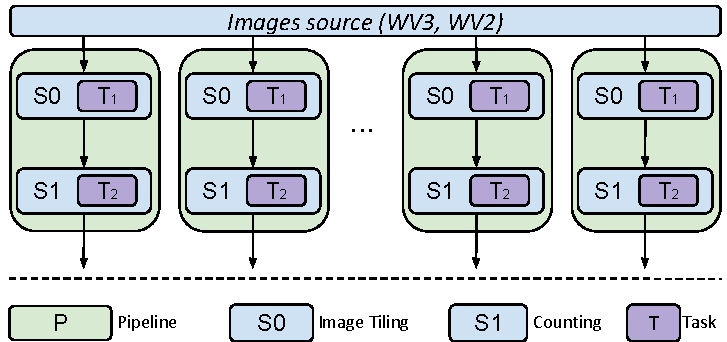
\includegraphics[width=\linewidth]{figures/designs/SealsDesign1.pdf}
        \caption{}
        \label{fig:seals_design1}
    \end{subfigure}\\
    ~ 
    \begin{subfigure}[b]{0.75\textwidth}
        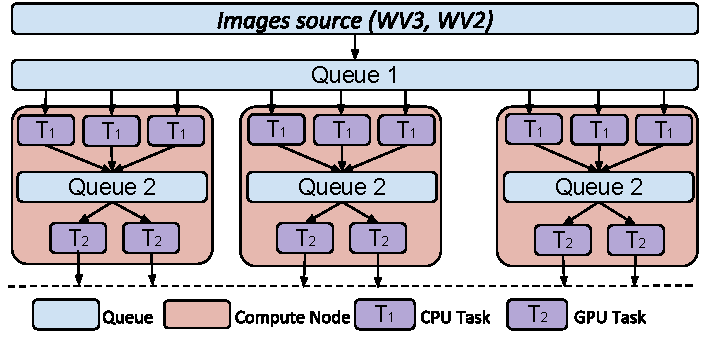
\includegraphics[width=\linewidth]{figures/designs/SealsDesign2.pdf}
        \caption{}\label{fig:seals_design2}
    \end{subfigure}\\
    ~ 
    \begin{subfigure}[b]{0.75\textwidth}
        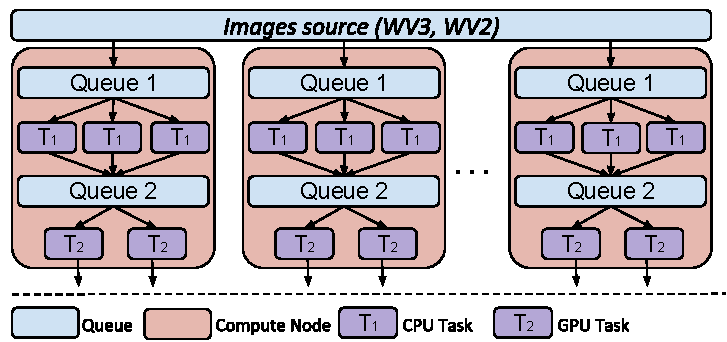
\includegraphics[width=\linewidth]{figures/designs/SealsDesign3.pdf}
        \caption{}\label{fig:seals_design3}
    \end{subfigure}
    \caption{Design approaches to implement the workflow required for the Seals use case.~\ref{fig:seals_design1}
        --\textbf{Design 1}: Pipeline, stage and task based design.~\ref{fig:seals_design2}
        --\textbf{Design 2}: Queue based design with a single queue for all the tiling tasks.~\ref{fig:seals_design3}
        --\textbf{Design 2.A}: Queue based design with multiple queues for the tiling tasks.}\label{fig:designs}
\end{figure}

% ---------------------------------------------------------------------------
\subsection{Design 1: One Image per Pipeline}
\label{ssec:approach1}\label{des1}


% ---------------------------------------------------------------------------
% Design
% ---------------------------------------------------------------------------

We specify the workflow for counting the number of seals in a set of images as a set of pipelines.
Each pipeline is composed of two stages, each with one type of task.
The task of the first stage gets an image as input and generates tiles of that image as output.
The task of the second stage gets the generated tiles as input, counts the number of seals found in each tile and outputs the aggregated result for the whole image.

Formally, we define two types of tasks:
\begin{itemize}
    \item $T_{1} = <I, f_{I}, t>$, where $I$ is an image, $f_{I}$ is a tiling function and $t$ is a set of tiles that correspond to $I$.
    \item $T_{2} = <t, f_{A}, S>$, where $f_{A}$ is a function that counts seals from a set of tiles and $S$ is the number of seals.
\end{itemize}


% ---------------------------------------------------------------------------
% Implementation
% ---------------------------------------------------------------------------
Tiling in $T_{1}$ is implemented with OpenCV~\cite{bradski2000opencv} and Rasterio~\cite{gillies2013rasterio} in Python.
Rasterio allows us to open and convert a GeoTIFF WV3 image to an array.
The array is then partitioned to sub\-arrays based on a user-specified scaling factor.
Each sub\-array is converted to an compressed image via OpenCV routines and saved to the filesystem.

Seal counting in $T_{2}$ is performed via a Convolutional Neural Network (CNN) implemented with PyTorch~\cite{paszke2017automatic}.
The CNN counts the number of seals for each tile of an input image.
When all tiles are processed, the coordinates of the tiles are converted to the geographical coordinates of the image and saved in a file, along with the number of counted seals.
Note that the number of seals in an tile does not affect the execution of the network, i.e. the same number of operations will be executed.

Both tiling and seal counting implementations are invariant between the designs we consider.
This is consistent with the designs being task-based, i.e., each task exclusively encapsulates the capabilities required to perform a specific operation over an image or tile.
Thus, tasks are independent from the capabilities required to coordinate their execution, whether each task processes a single image or sequence of images.

We implemented Design~1 via EnTK, a workflow engine which exposes an API based on pipelines, stages, and tasks~\cite{balasubramanian2018harnessing}.
The user can define a set of pipelines, where each pipeline has a sequence of stages, and each stage has a set of tasks.
Stages are executed respecting their order in the pipeline while the tasks in each stage can execute concurrently, depending on resource availability.

For our use case, EnTK has three main advantages compared to other workflow engines:
\begin{inparaenum}[(1)]
    \item it exposes pipelines and tasks as first-order abstractions implemented in Python;
    \item it is specifically designed for concurrent management of up to $10^5$ pipelines; and
    \item it supports RADICAL-Pilot.
\end{inparaenum} 
Together, these features address the challenges of heterogeneity, scale and repeatability: users can encode multiple pipelines, each with different types of tasks, executing them at scale on HPC machines without explicitly coding parallelism and resource management.

When implemented in EnTK, the use case workflow maps to a set of pipelines, each with two stages $St_{1}$, $St_{2}$.
Each stage has one task $T_{1}$ and $T_{2}$ respectively.
The pipeline is defined as $P = (St_{1},St_{2})$.
For our use case the workflow consists of $N$ pipelines, where $N$ is the number of images.

Figure~\ref{fig:seals_design1} shows the workflow.
For each pipeline, EnTK submits the task of stage $St_{1}$ to the runtime system (RTS).
As soon as the task finishes, the task of stage $St_{2}$ is submitted for execution.
This design allows concurrent execution of pipelines and, as a result, concurrent analysis of images, one by each pipeline.
Since pipelines execute independently and concurrently, there are instances where $St_{1}$ of a pipeline executes at the same time as $St_{2}$ of another pipeline.

Design~1 has the potential to increase utilization of available resources as each compute node of the target HPC machine has multiple CPUs and GPUs.
Importantly, computing concurrency comes with the price of multiple reading and writing to the filesystem on which the dataset is stored.
This can cause I/O bottlenecks, especially if each task of each pipeline reads from and writes to the same filesystem, possibly over a network connection.

We used a tagged scheduler for EnTK's RTS to avoid I~/O bottlenecks.
This scheduler schedules $T_{1}$ of each pipeline on the first available compute node, and guarantees that the respective $T_{2}$ is scheduled on the same compute node.
As a result, compute/data affinity is guaranteed among co-located $T_{1}$ and $T_{2}$.
While this design avoids I~/O bottlenecks, it may reduce concurrency when the performance of the compute nodes and/or the tasks is heterogeneous: $T_{2}$ may have to wait to execute on a specific compute node while another node is free.


% ---------------------------------------------------------------------------
\subsection{Design 2: Multiple images per pipeline}\label{ssec:approach2}

Design~2 implements a queue-based design.
We introduce two tasks $T_{1}$ and $T_{2}$ as defined in~\S\ref{ssec:approach1}.
Contrary to Design 1, these tasks are started and then executed for as long as data and resources are available, processing input images at the rate taken to process each image.
The number of concurrent $T_{1}$ and $T_{2}$ depends on available resources, including CPUs, GPUs, and RAM.

For implementing Design~2, we do not need EnTK, as we submit a bag of $T_{1}$ and $T_{2}$ tasks via the RADICAL~-Pilot RTS, and manage the data movement between tasks via queues.
As shown in Fig.~\ref{fig:seals_design2}, Design 2 uses one queue (Queue 1) for the dataset, and another queue (Queue 2) for each compute node.
For each compute node, each $T_{1}$ pulls an image from Queue 1, tiles that image and then queues the resulting tiles to Queue 2.
The first available $T_{2}$ on that compute node, pulls those tiles from Queue 2, and counts the seals.

%To communicate data and control signals between queues and tasks, we defined a communication protocol with three entities: Sender, Receiver, and Queue. 
%Sender connects to Queue and pushes data.
%When done, Sender informs Queue and disconnects.
%Receiver connects to Queue and pulls data.
%If there are no data in Queue but Sender is connected, Receiver pulls a ``wait'' message, waits, and pulls again after a second.
%When there are no data in Queue or Sender is not connected to Queue, Receiver pulls an ``empty'' message, upon which it disconnects and terminates.
%This ensures that tasks are executing, even if starving, and that all tasks are gracefully terminating when all images are processed.

Note that Design~2 load balances $T_{1}$ tasks across compute nodes but  balances $T_{2}$ tasks only within each node.
For example, suppose that $T_{1}$ on compute node $A$ runs two times faster than $T_{1}$ on compute node $B$.
Since both tasks are pulling images from the same queue, $T_{1}$ of $A$ will process twice as many images as $T_{1}$ of $B$.
Both $T_{1}$ of $A$ and $B$ will execute for around the same amount of time until Queue 1 is empty, but Queue 2 of $A$ will be twice as large as Queue 2 of $B$.
$T_{2}$ tasks executing on $B$ will process half as many images as $T_{2}$ tasks on $A$, possibly running for a shorter period of time, depending on the time taken to process each image.

In principle, Design~2 can be modified to load balance also across Queue 2 but in practice, as discussed in~\S\ref{ssec:approach1}, this would produce I/O bottlenecks.
Load balancing across $T_{2}$ tasks would require for all tiles produced by $T_{1}$ tasks to be written to and read  from a  shared filesystem.
Keeping Queue 2 local to each compute node enables using the filesystem local to each compute node.

% ---------------------------------------------------------------------------
\subsubsection{Design 2.A: Uniform image dataset per pipeline}
\label{sssec:approach2a}

The lack of load balancing of $T_{2}$ tasks in Design 2 can be mitigated by introducing a queue in each node from where $T_{1}$ tasks pull images.
This allows early binding of images to compute nodes, i.e., deciding the distribution of images per node before executing $T_{1}$ and $T_{2}$.
As a result, the execution can be load balanced among all available nodes, depending on the correlation between image properties and image execution time.

Figure~\ref{fig:seals_design3} shows variation 2.A of Design~2.
The early binding of images to compute nodes introduces an overhead compared to using late binding via a single queue as in Design 2.
Nonetheless, depending on the strength of the correlation between image properties and execution time, design 2.A offers the opportunity to improve resource utilization.
While in Design 2 some node may end up waiting for another node to process a much larger Queue 2, in design 2.A this is avoided by guaranteeing that each compute node has an analogous payload to process.

\section{Experiments: Task Execution Time, Resource Utilization and Overheads}\label{sec:des_experiments}
%See if comparing performance is better.
We executed three experiments using GPU compute nodes of the XSEDE Bridges supercomputer.
These nodes offer 32 cores, 128 GB of RAM and two P100 Tesla GPUs.
We stored the dataset of the experiments and the output files on XSEDE Pylon5 Lustre filesystem.
We stored the tiles produced by the tiling tasks on the local filesystem of the compute nodes.
This way, we avoided creating a performance bottleneck by performing millions of reads and writes of $\approx700$~KB on Pylon5.
We submitted jobs requesting 4 compute nodes to keep the average queue time within a couple of days.
Requesting more nodes produced queue times in excess of a week.
In addition, we had full control over the nodes during execution and were not shared with other users.

The experiments dataset consists of $3,097$ images, ranging from $50$ to $2,770$~MB for a total of $\approx4$~TB of data.
The images size follows a normal distribution with a mean value of $1,304.85$~MB and standard deviation of $512.68$~MB.

For Design~1, 2 and 2.A described in~\S\ref{sec:design}, Experiment~1 models the execution time of the two tasks of our use case as a function of the image size (the only property of the images for which we found a correlation with execution time); Experiment~2 measures the total resource utilization of each design; and Experiment~3 characterizes the overheads of the middleware implementing each design.
Together, these experiments enable performance comparison across designs, allowing us to draw conclusions about the performance of heterogeneous task-based execution of data-driven workflows on HPC resources.

% ---------------------------------------------------------------------------
\subsection{Experiment~1: Design~1 Tasks Execution Time}
\label{ssec:des1analysis}

Fig.~\ref{fig:stage_0_execution} shows the execution time of the tiling task---defined as $T_{1}$ in~\S\ref{des1}---as a function of the image size.
We partition the set of images based on image size, obtaining 22 bins with a range of $125$~MB each starting from $50$~MB up to $2,800$~MB.
The average time taken to tile an image in each bin tends to increase with the size of the image.
The box-plots show some positive skew of the data with a number of data points  falling outside the assumed normal distribution.
There are also large standard deviations ($STD$, blue line) in most of the bins.
Thus, there is a weak correlation between task execution time and image size with a large spread  across all the image sizes.

\begin{figure}[t]
    \centering
    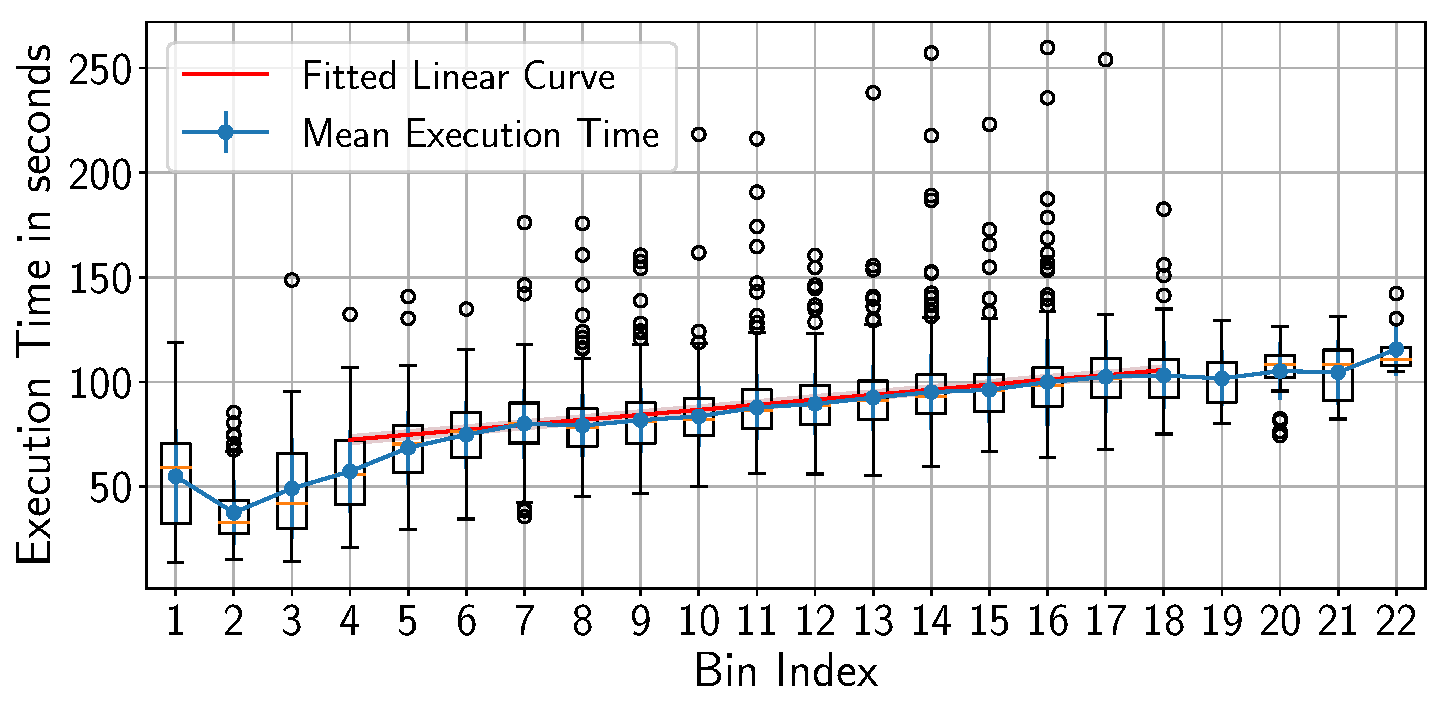
\includegraphics[width=0.75\textwidth]{figures/designs/stage_0_tx_box.pdf}
    \caption{Experiment~1, Design~1: Box-plots of $T_{1}$ execution time, mean and $STD$ for $125$~MB image size bins.
        Red line shows fitted linear function.}\label{fig:stage_0_execution}
\end{figure}

We explored the causes of the observed $STD$ by measuring how it varies in relation to the number of tiling tasks concurrently executing on the same node.
Fig.~\ref{fig:concurrency_test} shows the standard deviation of each bin of Fig.~\ref{fig:stage_0_execution}, based on the amount of used task concurrency.
We observe that $STD$ drops with increased concurrency but remains relatively stable between bins $\#6$ and $\#20$.
We attribute the initial dropping to how Lustre's caching improves the performance of an increasing number of concurrent requests.
Further, we observe that as the type of task and the compute node are the same across all our measures, the relatively stable and consistent $STD$ observed across degrees of task concurrency depends on fluctuations in the node performance.

\begin{figure}[t]
    \centering
    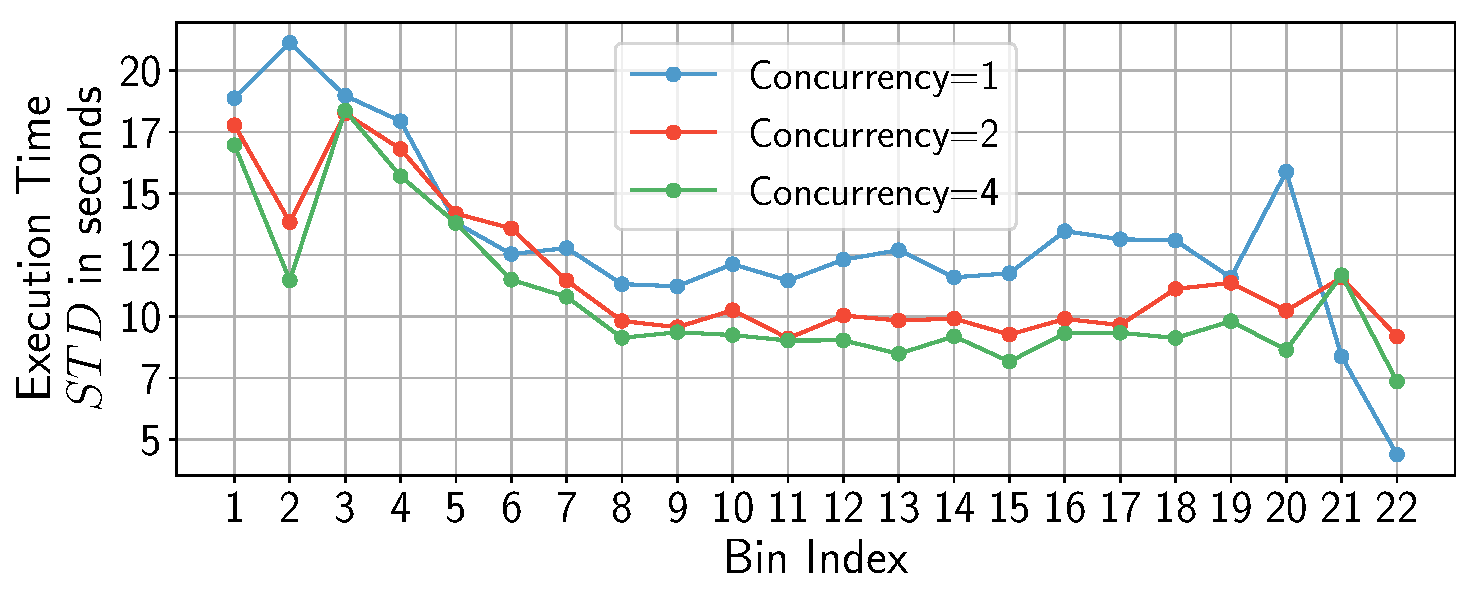
\includegraphics[width=.75\textwidth]{figures/designs/concerrency_std.pdf}
    \caption{$STD$ of $T_{1}$ execution time based on image size bin and number of concurrent tasks.
        Mostly dependent on compute node's performance and invariant across values of task concurrency.}\label{fig:concurrency_test}
\end{figure}

Fig.~\ref{fig:stage_0_execution} indicates that the execution time is a linear function of the image size between bin \#4 and bin \#18.
Bins $1-3$ and $19-23$ are not representative as the head and tail of the image sizes distribution contain less than $5\%$ of the image dataset.
We model the execution time as:
\begin{equation}
T(x) = \alpha \times x+\beta
\label{eq:des1_til}
\end{equation} where $x$ is the image size.


\begin{table*}[t]
    \scriptsize
    \centering
    \begin{tabular}{@{}cclrcl@{}}
        \toprule
        \textbf{Design}                                &
        \textbf{Fitted Data}                           &
        \textbf{$\alpha$ value}                        &
        \textbf{$\beta$ value}                         &
        \textbf{$R^2$ value}                           &
        \textbf{Figure}                                \\
        \midrule
        1                                              & 
        $T_{1}$                                  & 
        $1.92\times 10^{-2}$                           & 
        $60.49$                                        & 
        $0.97$                                         & 
        Fig.~\ref{fig:stage_0_execution}, red line     \\
        %
        1                                              & 
        $T_{2}$                                        & 
        $5.21\times 10^{-2}$                           & 
        $128.53$                                       & 
        $0.96$                                         & 
        Fig.~\ref{fig:stage_1_execution}, green line   \\
        %
        2                                              &
        $T_{1}$                                        &
        $3.17\times 10^{-2}$                           &
        $64.81$                                        &
        $0.92$                                         &
        Fig.~\ref{fig:stage_1_execution_des2}, red line     \\
		%
        2                                              &
        $T_{2}$                                        &
        $4.71\times 10^{-2}$                           &
        $95.83$                                        &
        $0.95$                                         &
        Fig.~\ref{fig:stage_2_execution_des2}, green line   \\
        2.A                                            &
        $T_{1}$                                        &
        $2.74\times 10^{-2}$                           &
        $49.03$                                        &
        $0.94$                                         &
        N/A     \\
		%
        2.A                                            &
        $T_{2}$.                                        &
        $4.80\times 10^{-2}$                           &
        $87.60$                                        &
        $0.95$                                         &
        N/A   \\
		\bottomrule
    \end{tabular}
    \caption{Fitted parameter values of Eq.~\ref{eq:des1_til} using a
             non-linear least squares algorithm to fit our experimental
             data.}\label{tab:fit_par_val}
\end{table*}

We found the parameter values of Eq.~\ref{eq:des1_til} by using a non-linear least squares algorithm to fit our experimental data, which are $\alpha= 1.92 \times 10^{-2}$, and $\beta = 60.49$ (see red line in Fig.~\ref{fig:stage_0_execution}).
$R^{2}$ of our fitting is $0.97$, showing a very good fit of the curve to the actual data.

The Standard Error of the estimation, $S_{error}$, reflects the precision of our regression.
The $S_{error}$ is equal to $1.93$, shown as the red shadow in Fig.~\ref{fig:stage_0_execution}.
From $R^{2}$ and $S_{error}$ we conclude that our estimated function is validated and is a good fit for the execution time of $T_{1}$ for Design~1.

% ---------------------------------------------------------------------------
% \subsubsection{\texorpdfstring{$St_2$}{St2} Stage Analysis}

Fig.~\ref{fig:stage_1_execution} shows the execution time of the seals counting task as a function of the image size.
Defined as $T_{2}$ in~\S\ref{des1}, this task presents a different behavior than $T_{1}$, as the code executed is different.
Note the slightly stronger positive skew of the data compared to that of Fig.~\ref{fig:stage_0_execution} but still consistent with our conclusion that deviations are mostly due to fluctuations in the compute node performance (i.e., different code but similar fluctuations).

\begin{figure}[t]
    \centering
    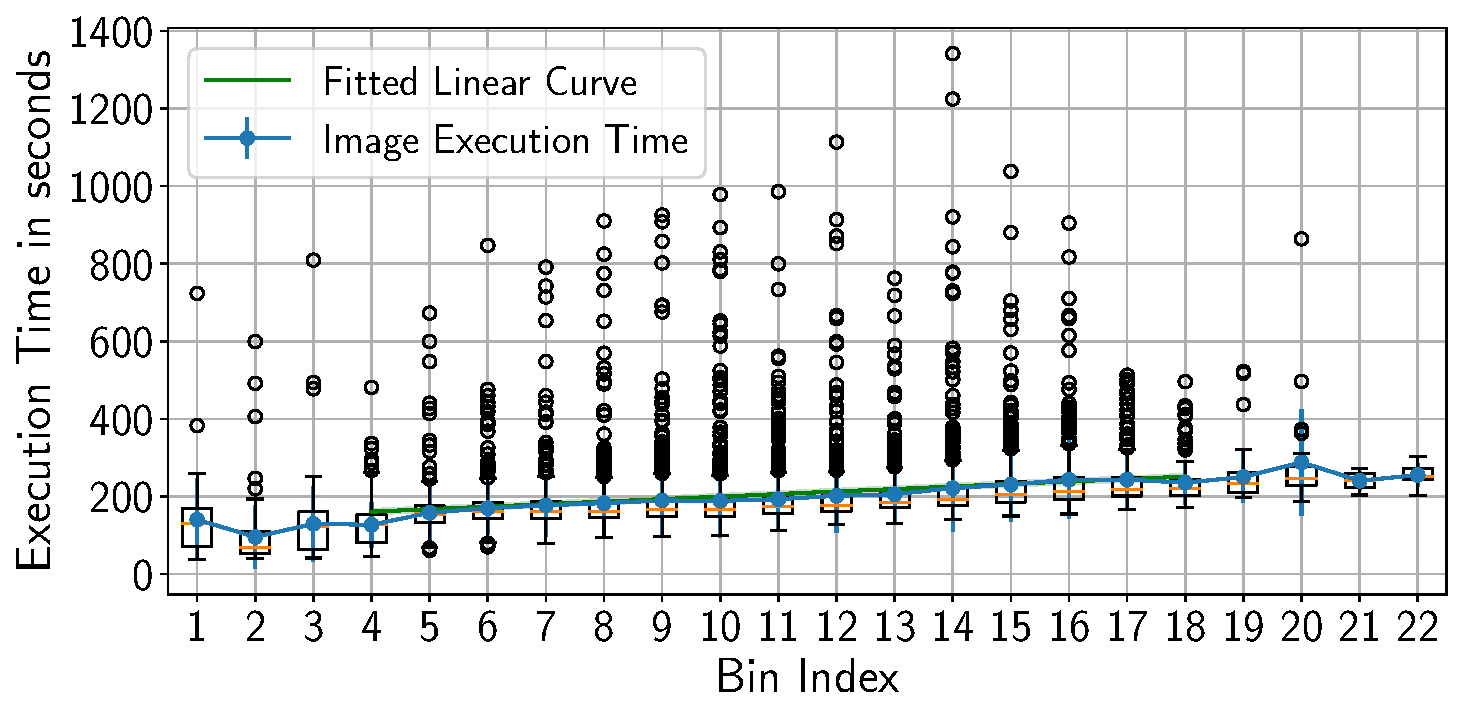
\includegraphics[width=0.75\textwidth]{figures/designs/stage_1_tx_box.pdf}
    \caption{Experiment~1, Design~1: Box-plots of $T_{2}$ execution time, mean and $STD$ for $125$~MB image size bins.
        Green line shows fitted linear function.}
    \label{fig:stage_1_execution}
\end{figure}

Similar to $T_{1}$, Fig.~\ref{fig:stage_1_execution} shows a weak correlation between the execution time of $T_{2}$ and image size.
In addition, the variance per bin is relatively similar across bins, as expected based on the analysis of $T_{1}$.
The box-plot and the mean execution time indicate that a linear function is a good candidate for a model of $T_{2}$.
As in Eq.~\ref{eq:des1_til}, we fitted a linear function to the execution time as a function of the image size for the same bins as $T_{1}$.

Using the same method we used with $T_{1}$, we produced the green line in Fig.~\ref{fig:stage_1_execution} with parameter values $\alpha = 5.21 \times 10^{-2}$ and $\beta = 128.53$.
$R^{2}$ is $0.96$, showing a good fit of the line to the actual data, while $S_{error}$ is $5.73$, slightly higher than for $T_{1}$.
As a result, we conclude that our estimated function is validated and is a good fit for the execution time of $T_{2}$ for Design~1.

% ---------------------------------------------------------------------------
\subsection{Experiment~1: Design~2 Tasks Execution Time}

Fig.~\ref{fig:stage_1_execution_des2} shows the execution time of $T_{1}$ as a function of the image size for Design~2.
In principle, design differences in middleware that execute tasks as independent programs should not directly affect task execution time.
In this type of middleware, task code is independent from that of the middleware: once tasks execute, the middleware waits for each task to return.
Nonetheless, in real scenarios with concurrency and heterogeneous tasks, the middleware may perform operations on multiple tasks while waiting for others to return.
Accordingly, in Design~2 we observe an execution time variation comparable to that observed with Design~1 but Fig.~\ref{fig:stage_1_execution_des2} shows a stronger positive skew of the data in Design~2 than Fig.~\ref{fig:stage_0_execution} in Design~1.

\begin{figure}[t]
    \centering
    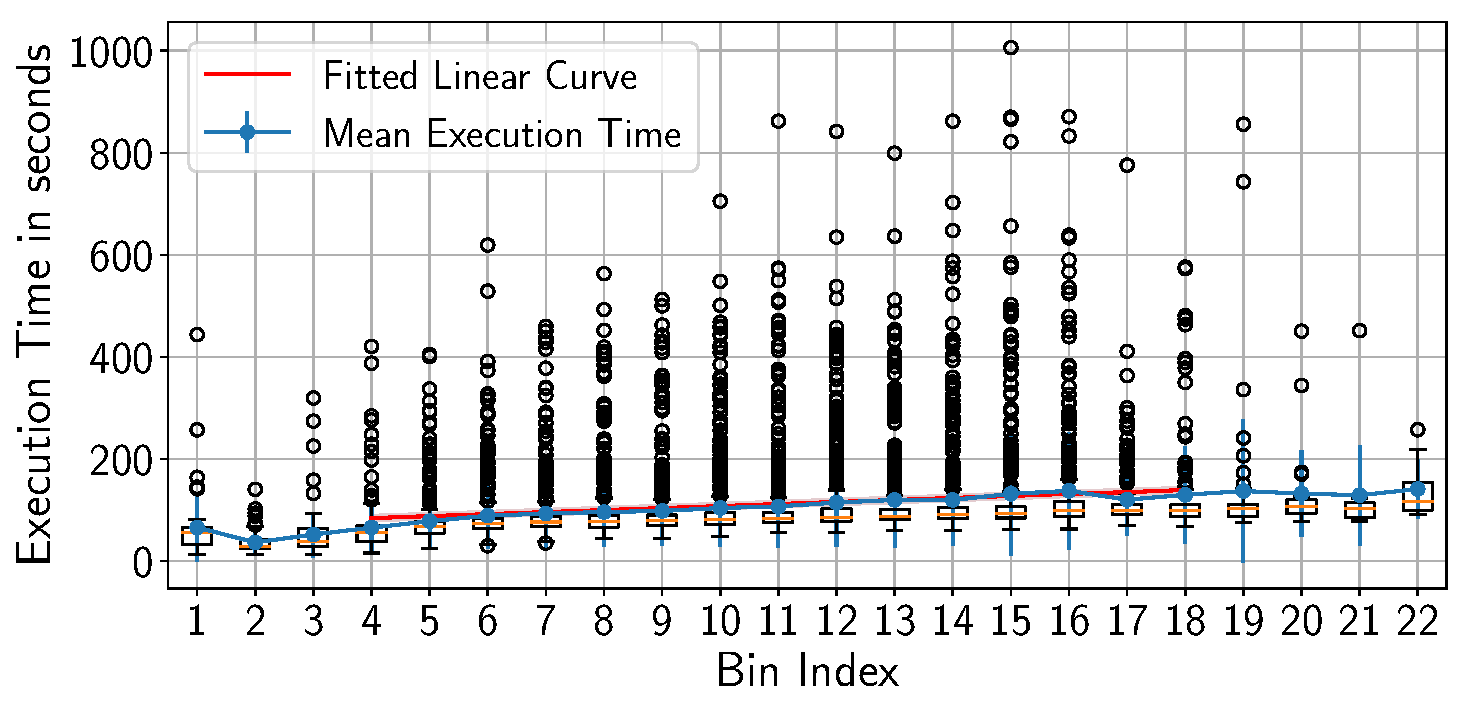
\includegraphics[width=0.75\textwidth]{figures/designs/stage_0_tx_box_des2.pdf}
    \caption{Experiment~1, Design~2: Box-plots of $T_{1}$ execution time, mean and $STD$ for $125$~MB image size bins.
        Red line shows fitted linear function.}\label{fig:stage_1_execution_des2}
\end{figure}


We investigated the positive skew of the data observed in Fig.~\ref{fig:stage_1_execution_des2} by comparing the system load of a compute node when executing the same number of tiling tasks in Design~1 and 2.
The system load of Design~2 was higher than that of Design~1.
Compute nodes have the same hardware and operating system, and run the same type and number of system programs.
As we used the same type of task, image and task concurrency, we conclude that the middleware implementing Design~2 uses more compute resources than that used for Design~1.
Due to concurrency, the middleware of Design~2 competes for resources with the tasks, momentarily slowing down their execution.
This is consistent with the architectural differences across the two designs: Design~2 requires resources to manage queues and data movement while Design~1 has only to schedule and launch tasks on each node.

We fitted Eq.~\ref{eq:des1_til} to the execution time of $T_1$ for Design~2, obtaining $\alpha = 3.174 \times 10^{-2}$ and $\beta = 64.81$.
The fitting produced the red line in Fig.~\ref{fig:stage_1_execution_des2}.
$R^{2}$ is $0.92$, showing a good fit of the curve to the data and $S_{error}$ is $5.50$, validating our estimated function.
$R^2$ and especially $S_{error}$ are worse compared to Design~1, an expected difference based on the positive skew of the data observed in Design~2.

% ------------
% \subsubsection{\texorpdfstring{$St_2$}{St2} Stage Analysis}

Fig.~\ref{fig:stage_2_execution_des2} shows that Design~2 also produces a much stronger positive skew of $T_{2}$ execution time compared to executing $T_{2}$ with Design~1.
$T_{2}$ executes on GPU and $T_{1}$ on CPU but their execution times produce comparable skew in Design~2.
This further supports our hypothesis that the long tail of the distribution of $T_{1}$ and especially $T_{2}$ execution times depends on the competition for main memory and I/O between the middleware implementing Design~2 and the executing tasks.


\begin{figure}[t]
    \centering
    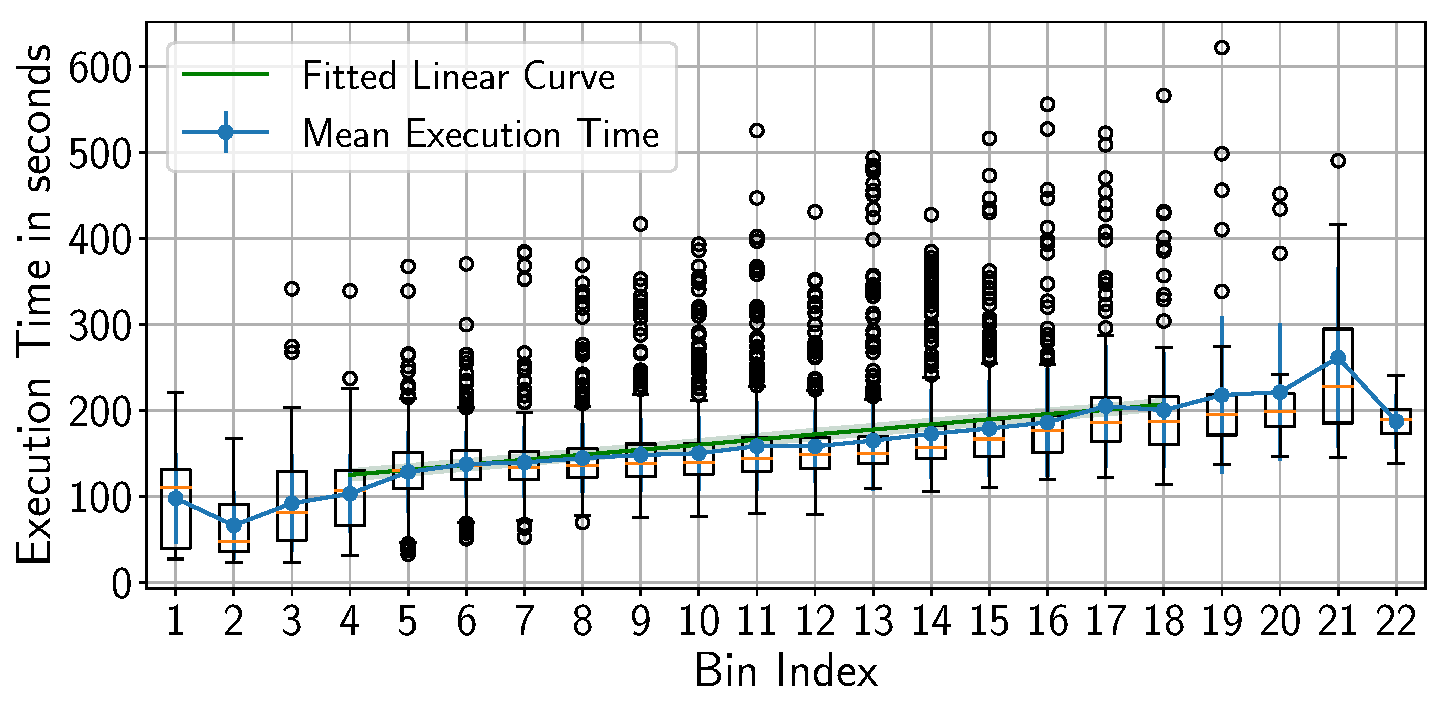
\includegraphics[width=0.75\textwidth]{figures/designs/stage_1_tx_box_des2.pdf}
    \caption{Experiment~1, Design~2: Box-plots of $T_{2}$ execution time, mean and $STD$ for $125$~MB image size bins.
        Green line shows fitted linear function.}\label{fig:stage_2_execution_des2}
\end{figure}

Fitting the model gives $\alpha = 4.71 \times 10^{-2}$ and $\beta = 95.83$.
$R^{2}$ is $0.95$ and $S_{error}$ of $5.96$.
As a result, the model is validated and a good candidate for the experimental data.
We attribute the difference between these values and those of the model of $T_{2}$ for Design~1 to the already described positive skew of execution times in Design~2.

% ------------
\subsubsection{Design~2.A} Similarly to the analysis in Design~1 and 2 we fitted data from Design~2.A to Eq.~\ref{eq:des1_til}.
For $T_{1}$ the fit gives $\alpha=2.74\times10^{-2}$ and $\beta=49.03$, with $R^{2}$ and $S_{error}$ of $0.94$ and $3.89$ respectively.
For $T_{2}$ the fit gives $\alpha=4.8\times10^{-2}$ and $\beta=87.36$, with $R^{2}=0.95$ and $S_{error}=6.19$.
Both models are therefore a good fit for the data and are validated.

The results of our experiments indicate that, on average and across multiple runs, there is a decrease in the execution time of $T_{1}$ and an increase in that of $T_{2}$ compared to Design~2.
Design~2.A requires one queue more than Design~2 for $T_{1}$ and therefore more resources for Design~2.A implementation.
This can explain the slowing of $T_{2}$ but not the speedup of $T_{1}$.
This requires further investigation, measuring whether the performance fluctuations of compute nodes are larger than measured so far.

As discussed in~\S\ref{ssec:approach2}, balancing of workflow execution differs between Design~2 and Design~2.A. Fig.~\ref{fig:design2_timeline} shows that each $T_{1}$ task can work on a different number of images but all $T_{1}$ tasks concurrently execute for a similar duration.
The four distributions in Fig.~\ref{fig:design2_timeline} also show that this balancing can result in different input distributions for each compute node, affecting the total execution time of $T_{2}$ tasks on each node.
Thus, Design~2 can create imbalances in the time to completion of $T_{2}$, as shown by the red bars in Fig.~\ref{fig:design2_timeline}.

\begin{figure}[t]
    \centering
    \begin{subfigure}[b]{0.75\textwidth}
        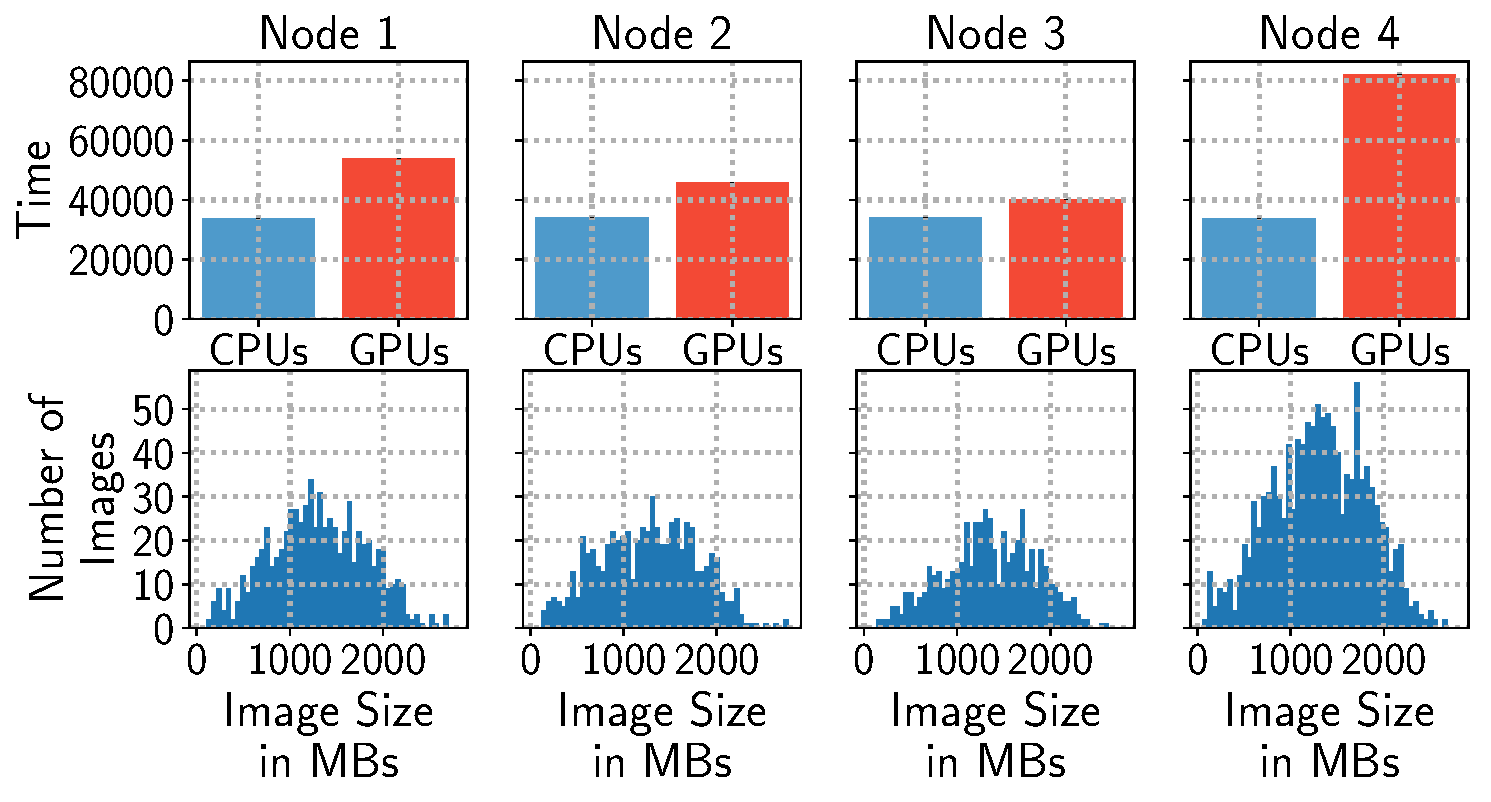
\includegraphics[width=\linewidth]{figures/designs/design2_timelines.pdf}
        \caption{}
        \label{fig:design2_timeline}
    \end{subfigure}\\
    ~ 
    \begin{subfigure}[b]{0.75\textwidth}
        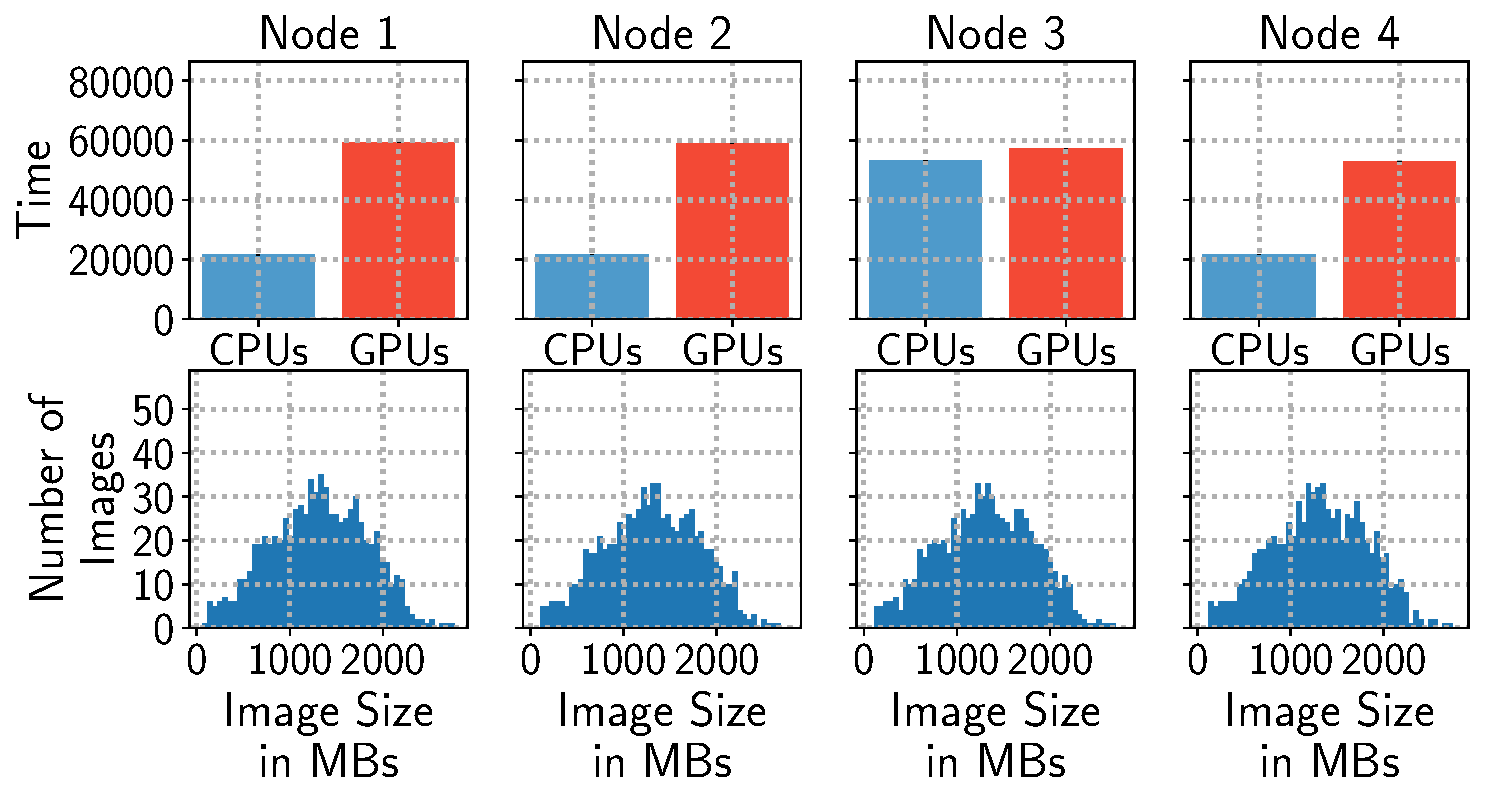
\includegraphics[width=\linewidth]{figures/designs/design2a_timelines.pdf}
        \caption{}
        \label{fig:design2a_timeline}
    \end{subfigure}
    \caption{Execution time of $T_{1}$ (blue) and $T_{2}$ (red),
        and distributions of image size per node for (a) Design~2 and (b)
        Design~2.A.}
    \label{fig:design_balancing}
\end{figure}


Design~2.A addresses these imbalances by early binding images to compute nodes.
Comparing the lower part of Fig.~\ref{fig:design2_timeline} and Fig.~\ref{fig:design2a_timeline} shows the difference between the distributions of image size for each node between Design~2 and 2.A.
In Design~2.A, due to the modeled correlation between time to completion and the size of the processed image, the similar distribution of the size of the images bound to each compute node balances the total processing time of the workflow across multiple nodes.

Note that Fig.~\ref{fig:design_balancing} shows just one of the runs we perform for this experiment.
Due to the random pulling of images from a global queue performed by Design~2, each run shows different distributions of image sizes across nodes, leading to large variations in the total execution time of the workflow.
Fig.~\ref{fig:design2a_timeline} shows also an abnormal behavior of one compute node: For images larger than $1.5$GBs, Node 3 CPU performance is markedly slower than other nodes when executing $T_{1}$.
Different from Design~2, Design~2.A can balance these fluctuations in $T_{1}$ as far as they don't starve $T_{2}$ tasks.

% ---------------------------------------------------------------------------
\subsection{Experiment~2: Resource Utilization Across Designs}\label{ssec:exp2}

Resource utilization varies across Design~1, 2 and 2.A. In Design~1, the RTS (RADICAL-Pilot) is responsible for scheduling and executing tasks.
$T_{1}$ is memory intensive and, as a consequence, we were able to concurrently execute 3 $T_{1}$ on each compute node, using only 3 of the 32 available cores.
We were instead able to execute 2 $T_{2}$ concurrently on each node, using all the available GPUs.
Assuming ideal concurrency among the 4 compute nodes we utilized in our experiments, the theoretical maximum utilization per node would be $10.6\%$ for CPUs and $100\%$ for GPUs.

Fig.~\ref{fig:Utilization} shows the actual resource utilization, in percent of resource type for each design.
The actual CPU utilization of Design~1 (Fig.~\ref{fig:design1util}) closely approximates theoretical maximum utilization but GPU utilization is well below the theoretical $100\%$.
GPUs are not utilized for almost an hour at the beginning of the execution and utilization decreases to $80\%$ some time after half of the total execution was completed.

Analysis shows that RADICAL-Pilot's scheduler did not schedule GPU tasks at the start of the execution even if GPU resources were available.
This points to an implementation issue and not to an inherent property of Design~1.
The drop in GPU utilization is instead explained by noticing that, as explained in~\S\ref{sec:design}, GPU tasks were pinned to specific compute nodes to avoid I/O bottlenecks.
Our experiments confirm that this indeed reduces utilization as some of the GPU tasks on some nodes take longer time to process than those on other nodes.

\begin{figure}[H]
    \centering
    \begin{subfigure}[b]{0.65\textwidth}
        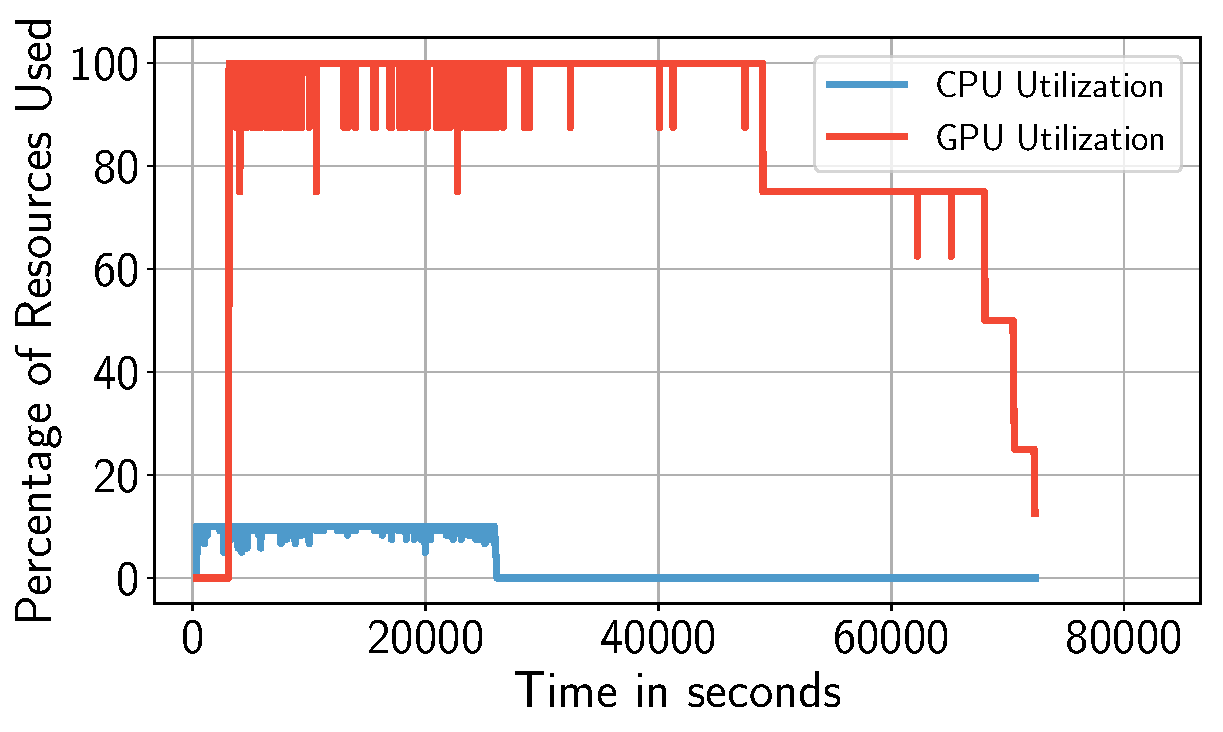
\includegraphics[width=\textwidth]{figures/designs/Design1Utilization.pdf}
        \caption{}
        \label{fig:design1util}
    \end{subfigure}\\
    ~ 
    \begin{subfigure}[b]{0.65\textwidth}
        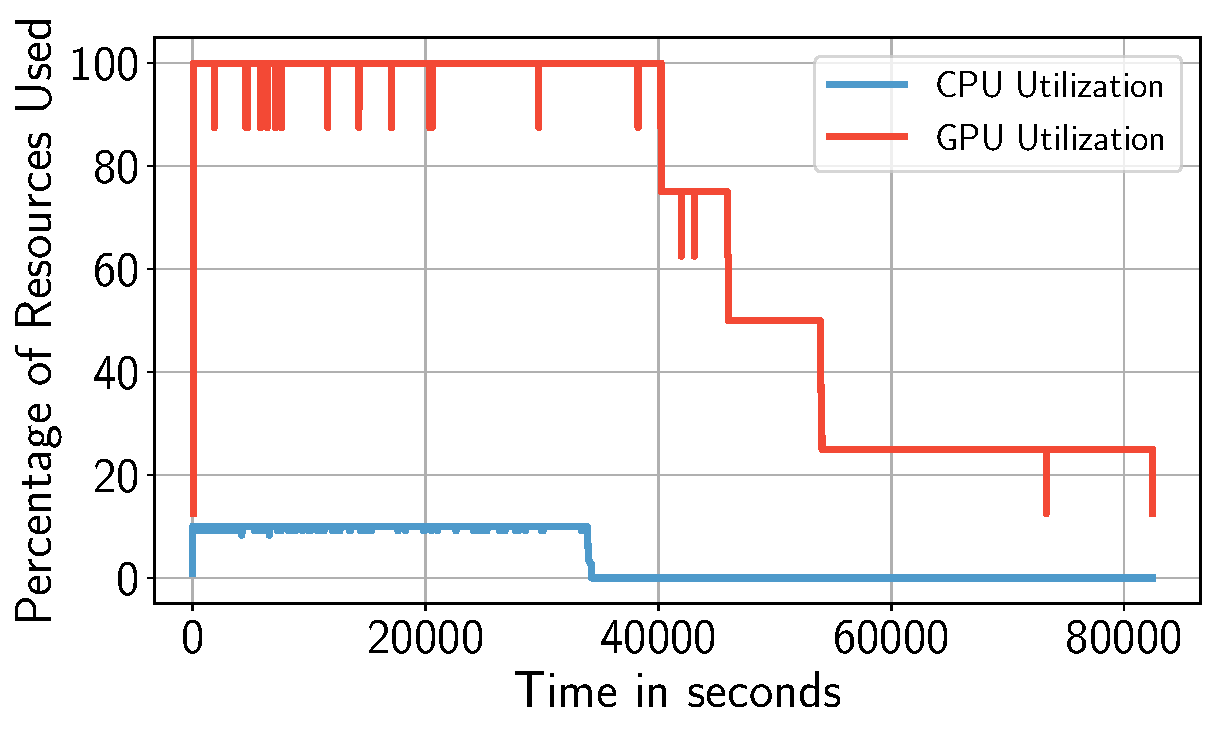
\includegraphics[width=\textwidth]{figures/designs/Design2Utilization.pdf}
        \caption{}
        \label{fig:design2util}
    \end{subfigure}\\
    ~ 
    \begin{subfigure}[b]{0.65\textwidth}
        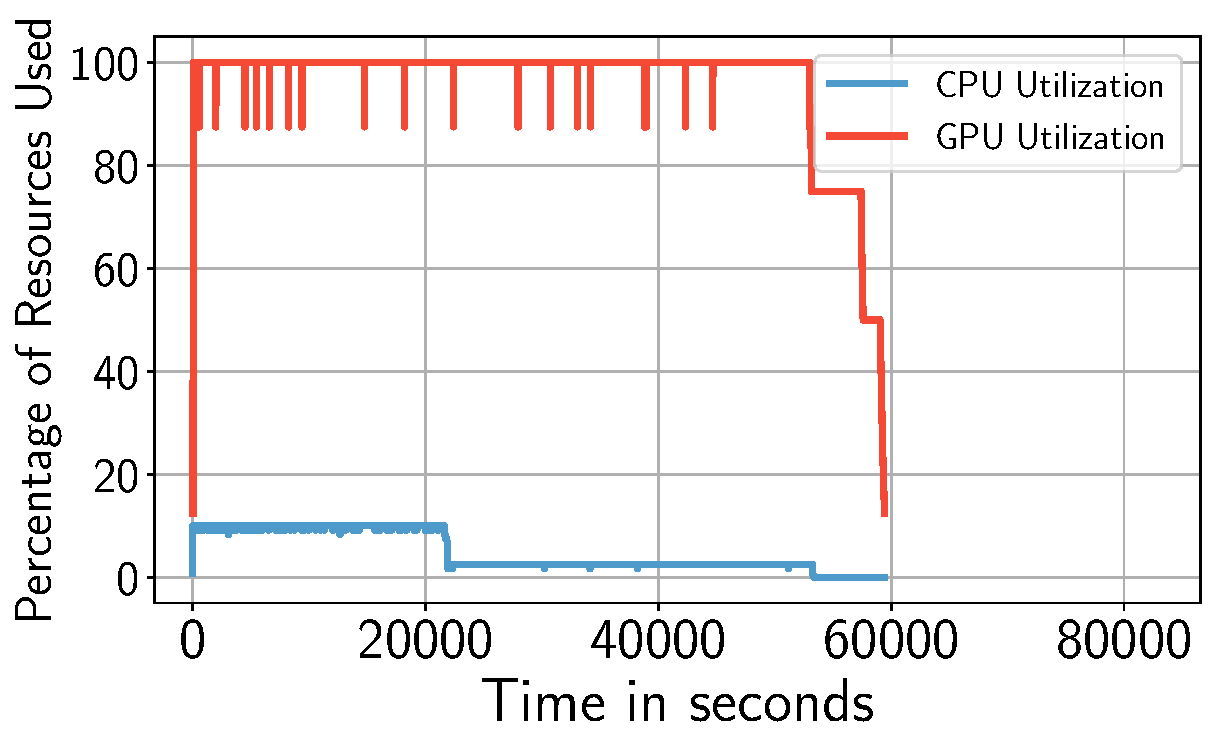
\includegraphics[width=\textwidth]{figures/designs/Design2AUtilization.pdf}
        \caption{}
        \label{fig:design2autil}
    \end{subfigure}
    \caption{Percentage of CPU and GPU utilization for: (a) Design~1; (b) Design~2, and (3) Design~2.A.}
    \label{fig:Utilization}
\end{figure}


Fig.~\ref{fig:design2util} shows resource utilization for a specific run of Design~2.
GPUs are utilized almost immediately as images are becoming available in the queues between $T_{1}$ and $T_{2}$, and this quickly leads to fully utilized resources.
CPUs are utilized for more time compared to Design~1, which is expected due to the longer execution times measured and explained in Experiment~1.
In addition, two GPUs ($25\%$ GPU utilization) are used for more than $20k$ seconds compared to other GPUs.
This shows that the additional execution time of that node was only due to the data size and not due to idle resource time.

Fig.~\ref{fig:design2autil} shows the resource utilization for a specific run of Design~2.A.
For 3 compute nodes out of 4, CPU utilization is shorter than for Design~1 and 2.
For the 4th compute node, CPU utilization is much longer as already explained when discussing $T_{1}$ execution time for Node 3 in Fig.~\ref{fig:design_balancing}, Experiment~1.
As already mentioned, the anomalous behavior of Node 3 supports our hypothesis that compute node performance fluctuations can be much wider than expected.

Fig.~\ref{fig:design2autil} shows that in Design~2.A GPUs are released faster compared to Design~1 and Design~2, leading to a GPU utilization above $90\%$.
As explained in Experiment~1, this is due to differences in data balancing among designs.
This shows the efficacy of two design choices for the concurrent execution of data-driven, compute-intense and heterogeneous workflows: early binding of data to node with balanced distribution of image size alongside the use of local filesystems for data sharing among tasks.

Note that drops in resource utilization are observed in all three designs.
In Design~1, although both CPUs and GPUs were used, in some cases CPU utilization dropped to 6 cores.
Our analysis showed that this happened when RADICAL-Pilot scheduled both CPU and GPU tasks, pointing to an inefficiency in the scheduler implementation.
Design~2 and 2.A CPU utilization drops mostly by one CPU where multiple tiling tasks try to pull from the queue at the same time.
This confirms our conclusions in Experiment~1 about resource competition between middleware and executing tasks.
In all designs, there is no significant fluctuations in GPU utilization, although there are more often in Design~1 when CPU and GPUs are used concurrently.

% ---------------------------------------------------------------------------
\subsection{Experiment~3: Designs Implementation Overheads}\label{ssec:exp3}. 

This experiment studies how the total execution time of our use case workflow varies across Design~1, 2 and 2.A. Fig.~\ref{fig:ttx} shows that Design~1 and 2 have similar total time to execution within error bars, while Design~2.A improves on Design~2 and both are substantially faster than Design~1.
The discussion of Experiment~1 and 2 results explains how these differences relate to the differences in the execution time of $T_{1}$ and $T_{2}$ tasks, and execution concurrency respectively.

\begin{figure}[H]
    \centering
    \begin{subfigure}{0.75\textwidth}
        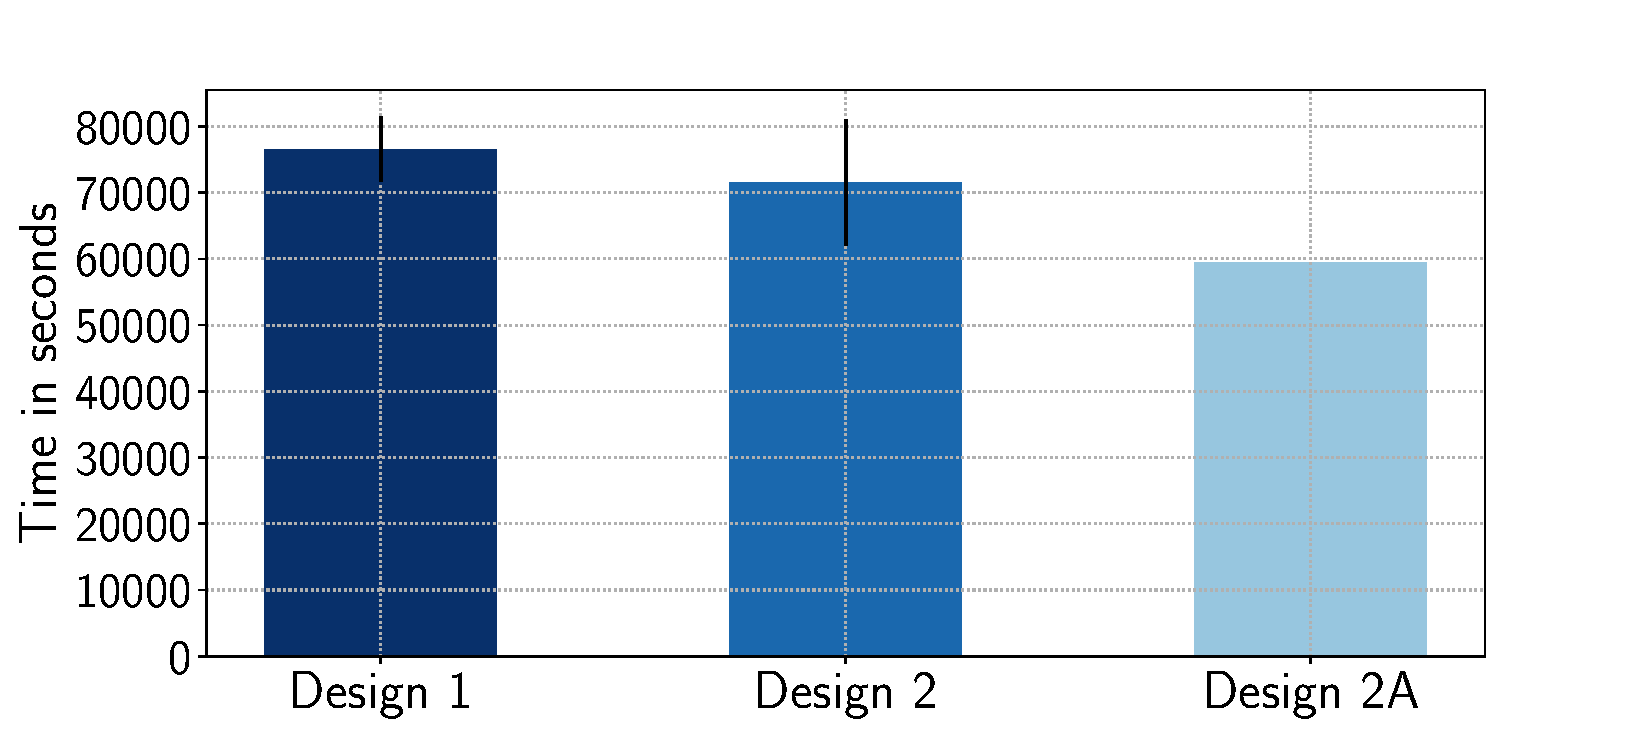
\includegraphics[width=\textwidth]{figures/designs/ttx.pdf}
        \caption{}
        \label{fig:ttx}
    \end{subfigure}\\
    ~
    \begin{subfigure}{0.75\textwidth}
        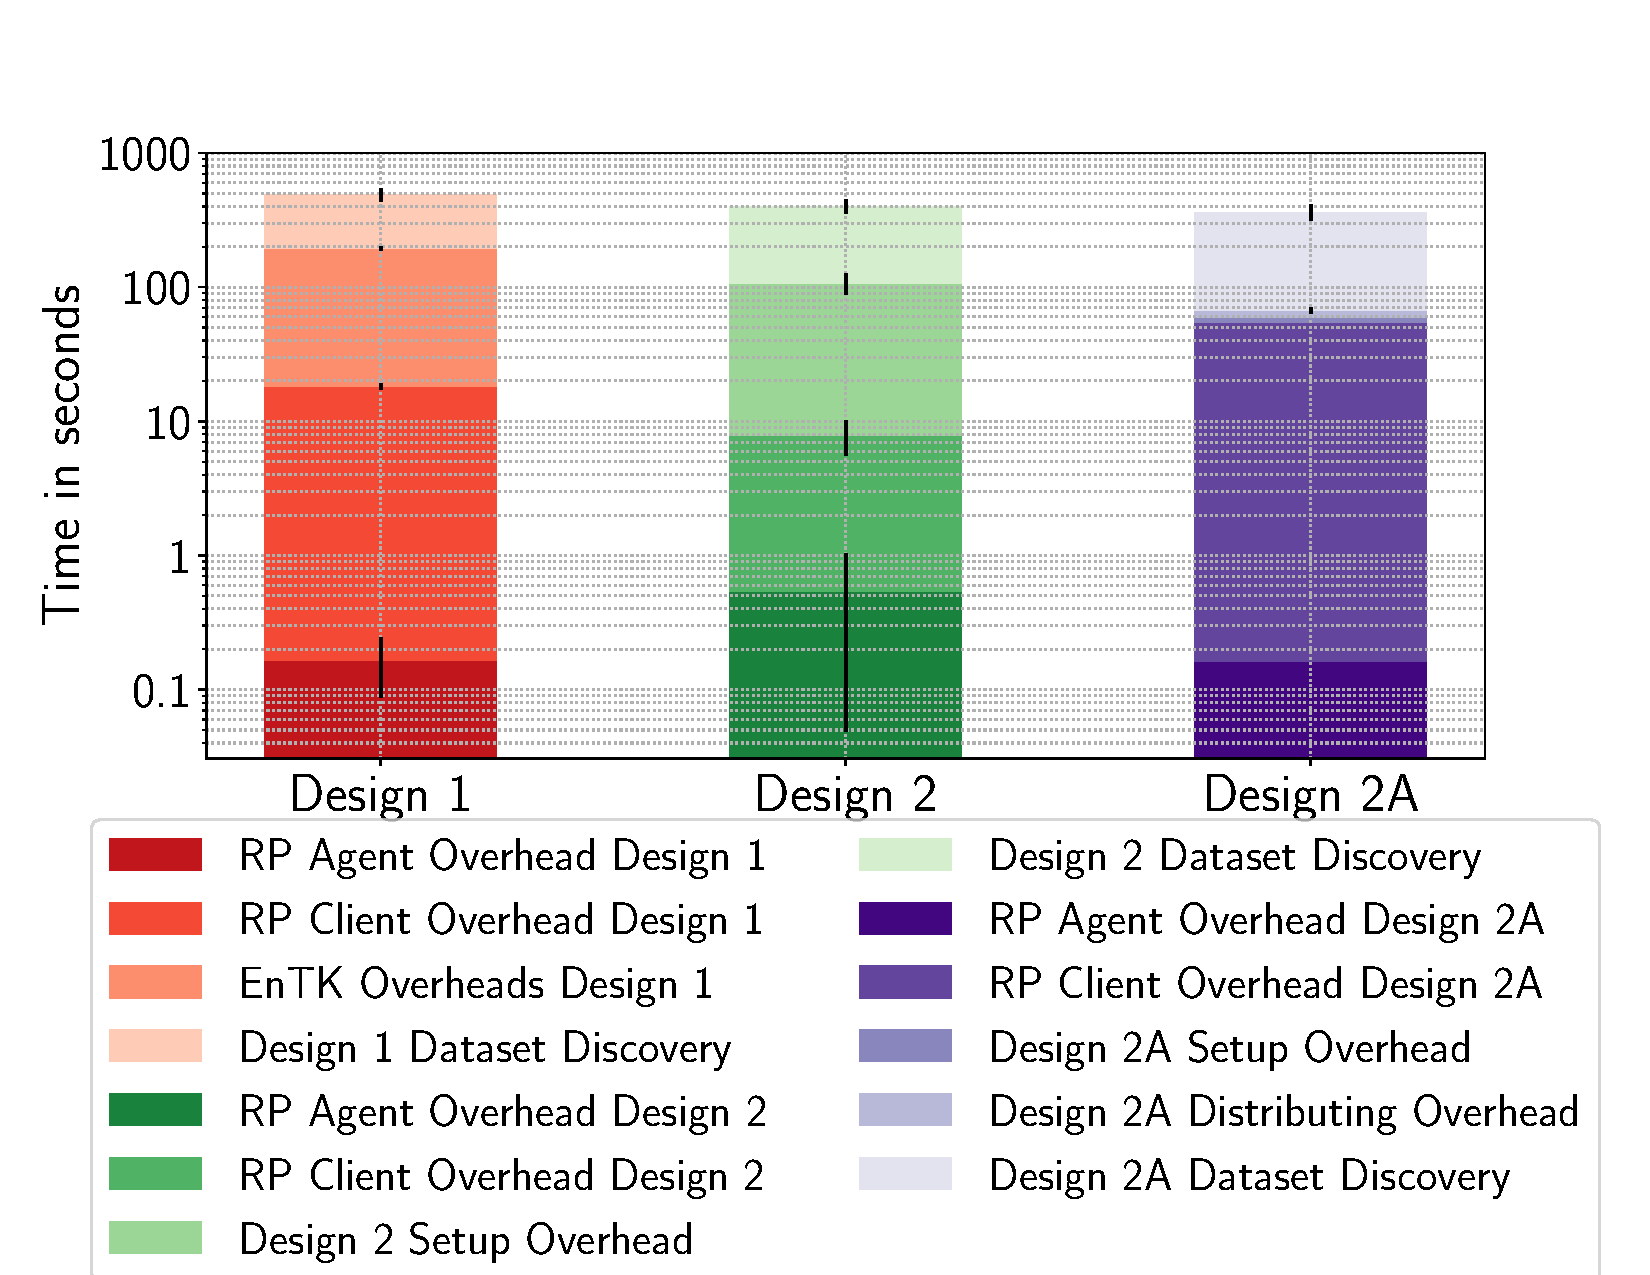
\includegraphics[width=\textwidth]{figures/designs/overheads.pdf}
        \caption{}
        \label{fig:overheads}
    \end{subfigure}
    \caption{(a) Total execution time of Design~1, 2 and 2.A. Design~1 and 2 have similar performance, Design~2.A is the fastest.
        (b) Overheads of Design~1, 2 and 2.A are at least two orders of magnitude less than the total execution time.}\label{fig:overall_performance}
\end{figure}


Fig.~\ref{fig:overheads} shows the overheads of each design implementation.
All three designs overheads are at least two orders of magnitude smaller than the total time to execution.
A common overhead between all designs is the ``Dataset Discovery Overhead''.
This overhead is the time needed to list the dataset and it is proportional to the size of the dataset. 
RADICAL-Pilot has two main components: Agent and Client.
RADICAL-Pilot Agent's overhead is less than a second in all designs while RADICAL-Pilot Client's overhead is in the order of seconds for all three designs.
The latter overhead is proportional to the number of tasks submitted simultaneously to RADICAL-Pilot Agent.

EnTK's overhead in Design~1 includes the time to: (1) create the workflow consisting of $3.1k$ independent pipelines; (2) start EnTK's components; and (3) submit the tasks that are ready to be executed to RADICAL-Pilot. 
This overhead is proportional to the number of tasks in the first stage of a pipeline, and the number of pipelines in the workflow.
EnTK does not currently support partial workflow submission, which would allow us to submit the minimum number of tasks to fully utilize the resources before submitting the rest.
Experiments should be performed to measure the offset between resource utilization optimization and increased time spent in communicating between EnTK and RADICAL-Pilot.

Fig.~\ref{fig:overheads} shows that the dominant overheads of Design~2 is ``Design~2 Setup Overhead''.
This overhead includes setting up and starting queues in each compute node, and starting and shutting down both $T_{1}$ and $T_{2}$ tasks on each node.
Setting up and starting the queues accounts for most of the overhead as we use a conservative waiting time to assure that all the queues are up and ready.
%This can be optimized further reducing the impact of this overhead.

Alongside the overheads already discussed, Design~2.A also introduces an overhead called ``Design~2.A Distributing Overhead'' when partitioning and distributing the dataset over separate nodes.
The average time of this overhead is $7.5$ seconds, with a standard deviation of $3.71$ and is proportional to the dataset and the number of available compute nodes.

In general, Design~2.A shows the best and more stable performance, in terms of overheads, resource utilization, load balancing and total time to execution.
Although Design~2 has similar overheads, even assuming minimization of Setup Overhead, it does not guarantee load balancing as done instead by 2.A.
Design 1 separates the execution in independent pipelines that are independently executed by the runtime system on any available resource.
Based on the results of our analysis, both EnTK and RADICAL-Pilot can be configured to implement early binding of images to each compute node as done in Design~2.A.
Nonetheless, Design~1 would still require executing a task for each image, imposing bootstrap and tear down overheads for each task.

\section{Discussion and Conclusions}
\label{sec:des_concl}

While designs 1, 2 and 2.A successfully support the execution of the paradigmatic workflow described in~\S\ref{sec:ucase}, our experiments show that for the metrics considered, Design~2.A is the one offering the better overall performance.
Generalizing this result, use cases that are both data-driven and compute-intense benefit from early binding of data to compute node so to maximize data and compute affinity and equally balance input across nodes.
This approach minimizes the overall time to completion of this type of workflows while maximizing resource utilization.

Our analysis also shows the limits of an approach where pipelines, i.e., compute tasks, are late bound to compute nodes.
In program-based designs, the overhead of bootstrapping programs needs to be minimized insuring that each pipeline processes as much input as possible (e.g. images).
In presence of large amount of data, late binding implies copying, replicating or accessing data over network and at runtime.
We showed that, in contemporary HPC infrastructures, this is too costly both for resource utilization and total time to completion.

When executing workflows as part of a computational campaign, it is important to efficiently utilize available resources.
Our design evaluation provides us with information on how to implement the workflows of a campaign effectively.
In addition, our overheads characterization provides us with a baseline to evaluate the production grade workflow implementations.


%Infrastructure-wise, our experiments show the limits imposed by an unbalance between number of CPU cores and available memory.
%Given data-driven computation where multi GB images need processing, we were able to use just $10\%$ of the available cores due to the amount of RAM required.
%This applies also to the unbalance between CPUs and GPUs: use cases with heterogeneous tasks would benefit from a n higher GPU/CPU ratio.

%These results apply to the evaluation of the design of existing and future computing frameworks. 
%For example, we are extending both EnTK and RADICAL-Pilot to implement Design~2.A.
%We will use our overheads characterization as a baseline to evaluate our production-grade implementation and further improve the efficiency of our middleware. 
%Further, we will apply the presented experimental methodology to other use cases and infrastructures, measuring the trade offs imposed by other types of task heterogeneity, including multi-core or multi-GPU tasks that extends beyond a single compute node.


%%%%%%%%%%%%%%%%%%%%%%%%%%%%%%%%%%%%%%%%%%%%%%%%%%%%%%%%%%%%%%%%%%%%%%%%%%%%%%%%
%For our CNN architecture, we use a U-Net~\cite{ronneberger2015u} variant that counts seals with an added regression branch and locates them using a seal intensity heat map.
%To train our CNN, we use a training set of 53 WV03 images, with $88k$ hand-labeled tiles, where every tile has a correspondent seal count and a class label (i.e., seal vs. non-seal).
%For hyper-parameter search, we train CNN variants for 75 epochs (i.e., 75 complete runs through the training set) using an Adam optimizer~\cite{kingma2014adam} with a learning rate of $10^{-3}$ and tested against a validation set.
%The validation set consists of $10\%$ of the training set.
%In addition, we randomized the WV03 image selection so that a validation tile does not overlap with a training one.
%Testing was performed on 5 WV03 images.
%Double observer seal counting was performed and model detection results were compared to observer consensus detections.
%Furthermore, we avoid double counting by setting a minimum distance boundary between neighboring seals and keeping those where the model was more confident.


% ---------------------------------------------------------
% CHAPTER 5
% ---------------------------------------------------------
\chapter{Scientific Computational Campaigns on HPC Platforms}
\label{ch:cmanager}
% !TEX root = main.tex

In the previous chapters, we discussed the requirements and support of
data- and compute-intensive workflows on high performance computing (HPC)
resources. When considering actual research, scientific projects require to
execute multiple workflows at scale and potentially for long period of time.
Usually, workflows are first developed, tested and executed for small scale
problems which can be verified theoretically. When ready, multiple workflows
are executed, potentially concurrently, at production scale for long periods
of time on the target HPC machine(s) while trying to achieve an objective.
This poses unprecedented computing challenges, shifting the problem from
enabling the effective and efficient execution of a single workflow at scale,
to managing the execution of a computational campaign.

The challenges users face when executing a computational campaign include, but
are not limited to, deciding an execution plan, submitting, executing and
monitoring workflows, and transferring data among resources. Workflow submission
requires users to have knowledge of submission systems, which generally differ
among HPC resources. Furthermore, users have to connect to those resources to
get information about the execution of workflows. Lastly, users have to
establish an execution plan which defines when each workflow will be executed
and on which HPC resource, with workflows potentially executing concurrently. A
campaign manager which, given a computational campaign and a set of resources,
creates an execution plan, submits, executes and monitors workflows on HPC
resources can address those challenges.

Existing campaign managers make assumptions about the resources and middleware
they are utilizing. In addition, they are monolithic software systems, despite
their modular design, and tend to be domain specific. For example,
PanDA~\cite{maeno2008panda}, Pegasus~\cite{deelman2015pegasus}, and
glideinWMS~\cite{sfiligoi2008glidein} are not easily extensible to use other
capabilities or runtime systems. QCFractal~\cite{qcfractal} is built to be
extensible and be able to interface with different workflow and workload
management systems, but remains domain specific.

In response to the limitations of existing campaign managers---monolithic
design, domain specific support, and dependence on specific resource and
middleware---we design and prototype a new campaign manager (CM). As our
CM has to support use cases from different scientific domains,
such as molecular dynamics, earth sciences and high energy physics on
potentially heterogeneous and diverse resources, the design and functionality
space grow exponentially. A prototype allows us to identify the most important
components and functionalities to support our use cases. Further, we can quickly
implement and test the CM without necessarily considering any
performance and data management requirements that may arise when executing an
actual campaign on actual production infrastructures. Finally, a prototype
allows us to tune parts of the CM with minimal engineering cost.

The CM prototype is domain agnostic as its design does not depend
on requirements from any specific scientific domain. In addition, our prototype
is designed by following the building blocks
approach~\cite{turilli2019middleware}. In this way, the prototype is agnostic
and makes no assumptions about the workflow management framework used to manage
the execution of individual workflows, as well as the type of resources used.

The chapter is organized as follows: \S~\ref{sec:cm_rw} discusses the current
solutions in executing computational campaigns. In \S~\ref{sec:cm_req}, we discuss the
supported use cases and the CM requirements.
\S~\ref{sec:cm_des} describes the building blocks approach and the design
of the CM. In \S~\ref{sec:cm_impl} we describe the
implementation of the CM prototype and we characterize its
baseline performance. We close the chapter with our conclusions in
Section~\ref{sec:cm_concl}.

\section{Related Work}

Currently, many software systems support computational campaigns. Among those,
PanDA~\cite{maeno2008panda}, DIRAC~\cite{casajus2010dirac},
QCFractal~\cite{qcfractal}, and glideinWMS~\cite{sfiligoi2008glidein} are the
ones with the widest adoption. These campaign managers, apart from
GlideInWMS~\cite{sfiligoi2008glidein}, are domain specific and make assumptions
about the underlying software stack and type of workflows to be executed. PanDA
WMS~\cite{maeno2008panda} mainly supports the distributed data analysis of data
produced by the ATLAS experiment~\cite{atlas} at the large hadron collider
(LHC). PanDA has been adapted to other use cases and projects, but it requires
major tailoring and dedicated support. This is also true for
DIRAC~\cite{tsaregorodtsev2003dirac}, which mainly supports the LHCb Monte Carlo
simulation production system at CERN. QCFractal~\cite{qcfractal} is a campaign
manager developed to execute large-scale quantum chemistry campaigns. It allows
users to define workflows based on the geometry of physical systems and execute
calculations, hiding the specifics of the software used.
GlideInWMS~\cite{sfiligoi2008glidein} is a more general purpose campaign manager
as it was specifically designed to support different use cases.

Existing campaign managers also support a plethora of computing resources,
including Grid resources, HPCs and Cloud. PanDA~\cite{maeno2008panda},
glideinWMS~\cite{sfiligoi2008glidein} and DIRAC~\cite{casajus2010dirac} mainly
support grid resources. PanDA has been extended to support
HPC~\cite{de2015future, de2016accelerating} and cloud
resources~\cite{de2016accelerating}, while glideinWMS~\cite{sfiligoi2008glidein}
supports only cloud resources. QCFractal~\cite{qcfractal} supports a set of
heterogeneous resources, including local campus clusters, and HPC and
cloud resources.

Workflow management frameworks such as Pegasus~\cite{deelman2015pegasus} and
Balsam~\cite{salim2019balsam} support the concurrent execution of multiple
workflows on HPC resources. Both frameworks allow users to submit multiple
workflows concurrently for execution but Balsam also provide multitenancy
capabilities, where multiple users can submit jobs for execution under the same
workflow. Despite this capabilities, both frameworks execute workflows as
independent entities but not as part of a computational campaign with a well
defined objective.

\section{Campaign Manager Requirements}
\label{sec:cm_req}

The space of data analysis of computational campaigns can be vast with different
scientific objectives, types and number of workflows and resources. We use three
real use cases with data analysis workflows to derive the requirements of the
CM prototype. The first use case supports quantum chemistry
campaigns (UC1), the second earth science (UC2) and the third data analysis
campaigns which analyze the data produced for the ATLAS experiment (UC3).

Quantum chemistry defines campaigns which execute workflows that perform
chemical computations on molecules to calculate their properties, e.g., energy.
These campaigns execute thousands of workflows, with up to 1000 executing at any
given point in time, on a number of resources~\cite{smith2020molssi}. Workflows
execution time varies between half-core hours up to 100-core hours, with
different levels of concurrency. In addition, users have access to resources
with several capabilities and not every workflow can be executed on every
resource. During the campaign definition, users may provide an initial workflow
priority and have to be sure that the campaign will finish within the given
resource allocation.

Earth science campaigns analyze imagery acquired via sensors from different
calendar years~\cite{paraskevakos2019workflow} to create time series of
ecological events, executing one workflow per imagery from a calendar year.
Their execution time varies from hours to a couple of days. Due to the volume of
the data, users have access to a small number of resources where imagery is
stored. While workflows analyze datasets based on the year they represent, a
specific execution order is not necessary as long as all datasets are analyzed.
The objective of this campaign is to analyze as many years of imagery as
possible, thus they target high throughput imagery per unit of time.

The third use case supports the execution of data analysis workflows from the
ATLAS experiment~\cite{atlas}. LHC produces data as particles collide inside its
detectors. These data are then analyzed by executing hundreds to thousands
workflows with different timescales and frequencies~\cite{borodin2015big}. In
addition, the analysis needs to happen within specific time boundaries, while
the detector is not operational. For example, one of the use cases described in
Ref.~\cite{borodin2015big} analyzes thousands of different datasets with
workflows running for months every yearly quarter. As a result, the objective of
this use case campaign is to finish all of its workflows within a specific
amount of time.

Based on these use cases, we derive a set of functional requirements for the
CM prototype. Table~\ref{tab:fun_reqs} shows a summary of the
functional requirements. The table defines a requirement identification number,
states the requirement and provides a description of each requirement. In
addition to this information, the table shows from which use case the
requirement is derived with ``G'' being a requirement that supports all three
use cases.

\begin{table}[t]
    \centering
    \scriptsize
    \begin{tabular}{@{}p{1.5cm}|p{2.8cm}p{1.5cm}p{6cm}@{}}
        \toprule
        \textbf{REQ ID} &\textbf{Requirement Algorithm} &\textbf{Use Case} & \textbf{Description} \\
        \midrule
         1 &
         Support campaign with O(1k) workflows &
         UC1 &
         The CM should be able to support campaigns with order of thousand workflows.
         Planning, execution and adaptation should be able to execute with such a campaign.\\
         2 &
         The CM should support at least two different planning algorithms. &
         G &
         Users/developers should be able to easily extend the planning capabilities with algorithms.\\
         3 &
         Support from 1 up to 100 resources &
         UC1-UC2 &
         The CM should be able to execute workflows on multiple resources concurrently.
         These resources can either be actual or emulated resources.\\
         4 &
         Plan should be derived for heterogeneous and homogeneous static resources in 5 minutes &
         G &
         The plan should be derived as soon as the user provides a campaign description.
         Plan should be derived in less than 5 minutes.\\
         5 &
         Plan should be derived and adapted for heterogeneous/homogeneous dynamic resources in 5 minutes &
         UC1 &
         The plan should be derived as soon as the user provides a campaign description.
         Plan should be derived in less than 5 minutes.
         In case the plan needs to be adapted, it should be adapted in less than 5 minutes.\\
         6 &
         Interface with different WMFs &
         G &
         The CM should be able to interface with different WMFs based on the specifics of the campaign. \\
         7 &
         Early bind workflows to resources &
         UC1 &
         The user may need to bind workflows to specific resources before executing the campaign.\\
         8 &
         Campaign objective is configurable &
         UC1 &
         While the campaign is executing, the objective may be adjusted based on user preferences.\\
         9 &
         Update the campaign during runtime &
         UC1-UC2 &
         The user may want to update the campaign while it is executing to add/remove workflows.\\
         10 &
         Resources may be added or removed during runtime &
         UC1 &
         The user may want to add/remove resources, she has gained/lost access to.\\
        \bottomrule
    \end{tabular}
    \caption{Campaign manager functional requirements.\label{tab:fun_reqs}}
\end{table}

\section{Campaign Manager Design}
\label{sec:cm_des}

This section discusses the design principles (\S\ref{ssec:building_blocks}) and
the architecture (\S\ref{ssec:cm_arch}) of the campaign manager prototype.

\subsection{Building Blocks Design Approach}
\label{ssec:building_blocks}

The building blocks approach, as described in Ref.~\cite{turilli2019middleware},
defines four design principles for software systems. Those are self-sufficiency,
interoperability, composability, and extensibility. Adhering to those principles
during the design and implementation phase of a software system allows for
greater software sustainability. In addition, it allows users not to tailor
their solutions to a specific software ecosystem and take full advantage of the
plethora of software that supports scientific computing.

Self-sufficiency and interoperability describe the characteristics of software
entities and functionalities. The entities are enough to stand alone and can
be reduced to a specific abstraction. The functionalities of each building
block are specific to the block and do not overlap with other blocks. As a
result, the CM design defines a set of components and that allow
it to execute a campaign to HPC resources without providing capabilities to
execute the individual workflows of the campaign or acquire the necessary
resources.

Composability and extensibility describe the communication and coordination
between building blocks and the generality of the generality of the blocks
components respectively. Blocks communicate information about their state,
events and errors. Based on this information alone building blocks are
coordinating with each other. As a result, the CM uses only the
state of the workflow execution to create the campaign state. Furthermore, its
components are designed to be general enough so that they can extended and
interface with different workflow execution engines as well as software
systems that execute computational campaigns.

\subsection{Campaign Manager Components}
\label{ssec:cm_arch}

We define three components as part of the CM prototype (see
Figure~\ref{fig:refarch}):
\begin{inparaenum}[(1)]
    \item a Planner;
    \item an Enactor; and
    \item a Bookkeeper.
\end{inparaenum}
Workflow execution will be managed by an existing workflow management framework
(WMF) on HPC resources. Each of these components supports a basic functionality
of the CM, such as executing individual workflows and monitoring
the campaign.

\begin{figure*}[t]
    \centering
    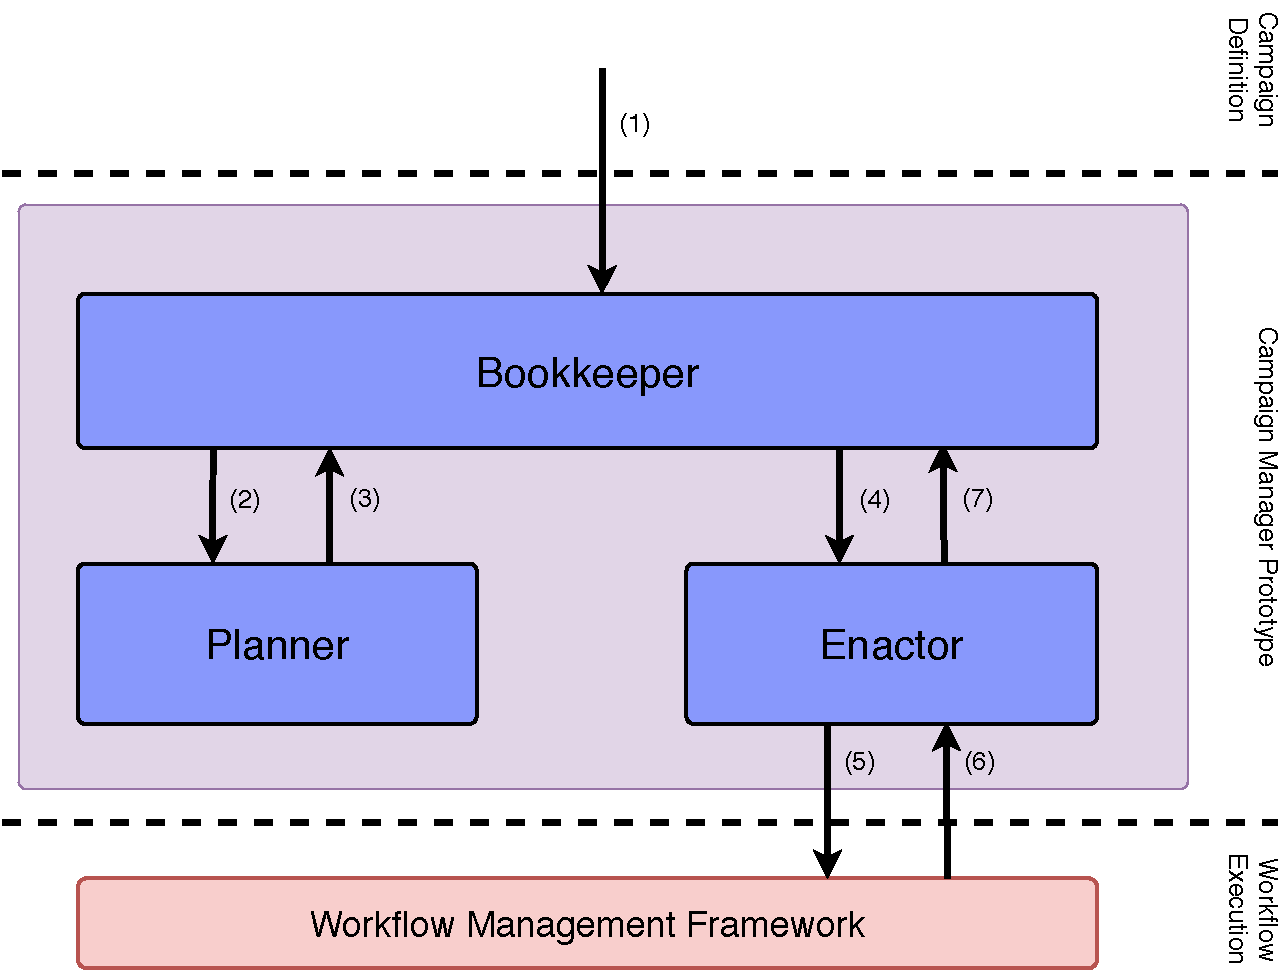
\includegraphics[width=.75\textwidth]{figures/manager/CEM_design.pdf}
    \caption{Reference Architecture of a Campaign Manager. Basic components of
        Campaign Manager (CM): (a) Planner, (b) Enactor and (c) Bookkeeper. CM
        communicates decisions to Workflows Management Framework. CM
        communicates with HPCs to execute parts of the
        campaign.}\label{fig:refarch}
\end{figure*}

The Planner component derives an execution plan based on a planning algorithm
and calculates the makespan for a campaign on a specific set of resources. The
Planner receives information about available resources and the workflows of the
campaign from the Bookkeeper component. The Planner does not adhere to a
specific planning algorithm, allowing different algorithms to be used, based on
the campaign's requirements and objective.

The Bookkeeper component is responsible for monitoring the execution of the
campaign. This component holds information about the state of the campaign, the
execution plan, the availability of resources, and the campaign's objective. The
state of the campaign is based on information about workflow execution provided
by the Enactor component. In addition, the Bookkeeper knows the state of the
resources utilized by the campaign at runtime and the state of the resources
that are planned to be used. Based on this information, the Bookkeeper checks
whether the campaign's objective can be achieved. Bookkeeper requests the
Planner to update the plan when changes in the campaign happen that
affect the effectiveness of a current plan or make the objective not achievable.
For example, the availability of one or more resources can change during
runtime, requiring a revision of the execution plan.

The Enactor component executes the campaign's workflows by interfacing with a
workflow management system (WMF). The Enactor receives a set of workflows from
the Bookkeeper, along with the resources on which the workflows will execute at
a given point in time. Based on this information, the Enactor submits the
workflows to the WMF for execution.

Initially, the Bookkeeper receives the description of a campaign
(Figure~\ref{fig:refarch} step 1) and passes information about resources and
workflows to the Planner (Figure~\ref{fig:refarch} step 2). As soon as a plan is
calculated, it is passed to the Bookkeeper (Figure~\ref{fig:refarch} step 3).
Then, the Bookkeeper passes the workflows and resources descriptions to the
Enactor (Figure~\ref{fig:refarch} step 4) and the Enactor passes that
information to the selected WMF for execution (Figure~\ref{fig:refarch} step 5).
When a workflow finishes to execute, the Enactor gets notified
(Figure~\ref{fig:refarch} step 6) and informs the Bookkeeper
(Figure~\ref{fig:refarch} step 7). Steps 4, 5, 6 and 7 repeat until all the
workflows have finished executing.

\section{Prototype Implementation and Performance Evaluation}
\label{sec:cm_impl}

Consistent with the design presented in~\S\ref{sec:cm_des}, we define three main
classes to implement the CM prototype. The Bookkeeper class
implements the capabilities of the Bookkeeper component, the Enactor class
interacts with a selected workflow engine to execute workflows on resources, and
the Planner class implements planning algorithms. In addition, the prototype
defines a state model for the campaign and the workflows.
Figure~\ref{fig:rcm_class_diagram} shows the class diagram of the prototype.
Each class also defines a set of data structures to support the execution of campaigns.

\begin{figure*}[t]
    \centering
    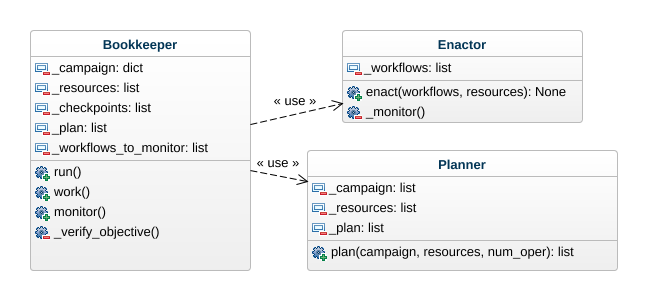
\includegraphics[width=.95\textwidth]{figures/manager/class_diagram.png}
    \caption{Class diagram of campaign manager prototype}\label{fig:rcm_class_diagram}
\end{figure*}

The states models provide information about the state of the execution. The
campaign state model (Figure~\ref{fig:CampaignStates}) has six states: (1)
\textit{new}, (2) \textit{planning}, (3) \textit{executing}, and (4)
\textit{done} or (5) \textit{canceled} or (6) \textit{failed}. A campaign is
considered \textit{new} when it is defined and no further action is taken. The
campaign transitions to the \textit{planning} state when a plan for its
execution is derived. As soon as the execution of the campaign starts, the state
of the campaign transitions to \textit{executing}. The final states are possible
termination states. When the campaign execution ends and the campaign objective
is achieved, the campaign transitions to the \textit{done} state. If the
objective cannot be achieved or there is a failure during the execution, the
state of the campaign changes to \textit{failed}. Lastly, the campaign state
goes to \textit{canceled} when the user cancels the execution of the campaign.
The code of the prototype is publicly available on Github~\cite{cm_git}.

\begin{figure*}[t]
    \centering
    \begin{subfigure}[b]{0.45\textwidth}
        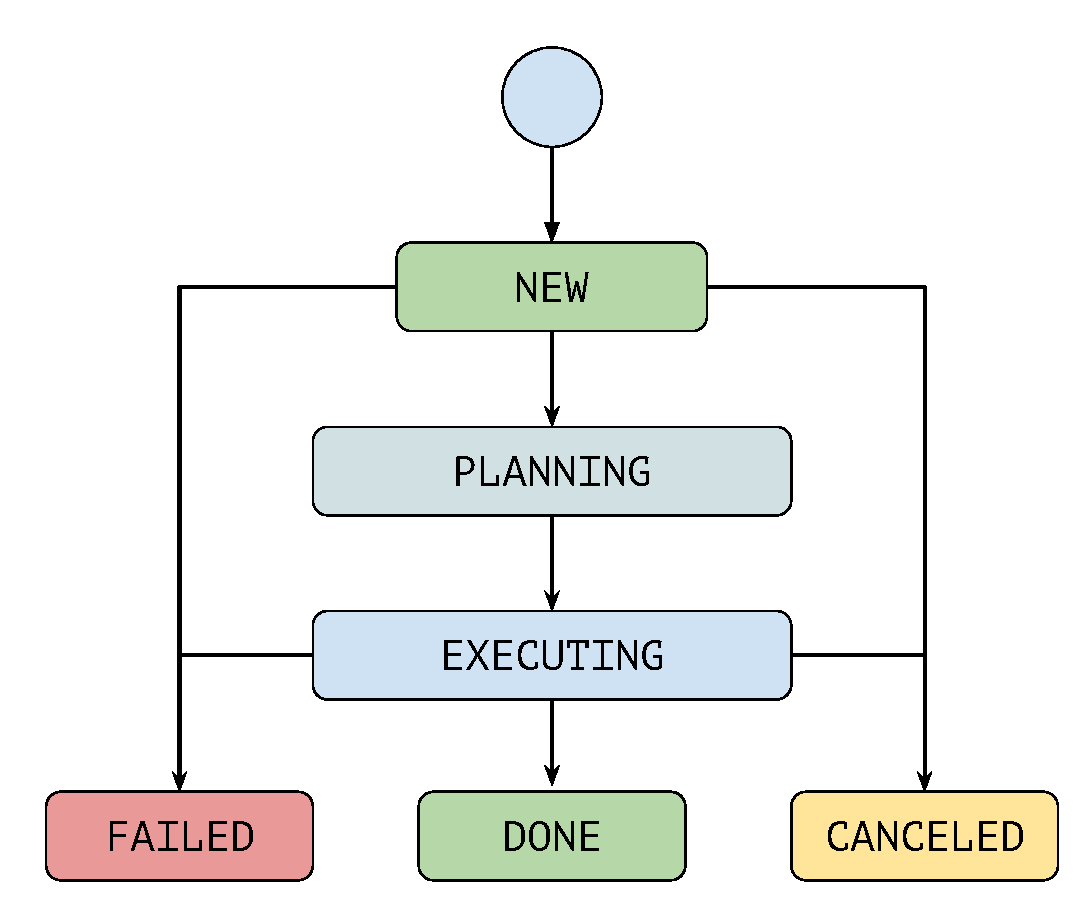
\includegraphics[width=.95\textwidth]{figures/manager/campaign-state-model.pdf}
        \caption{}
        \label{fig:CampaignStates}
    \end{subfigure}
    ~
    \begin{subfigure}[b]{0.45\textwidth}
        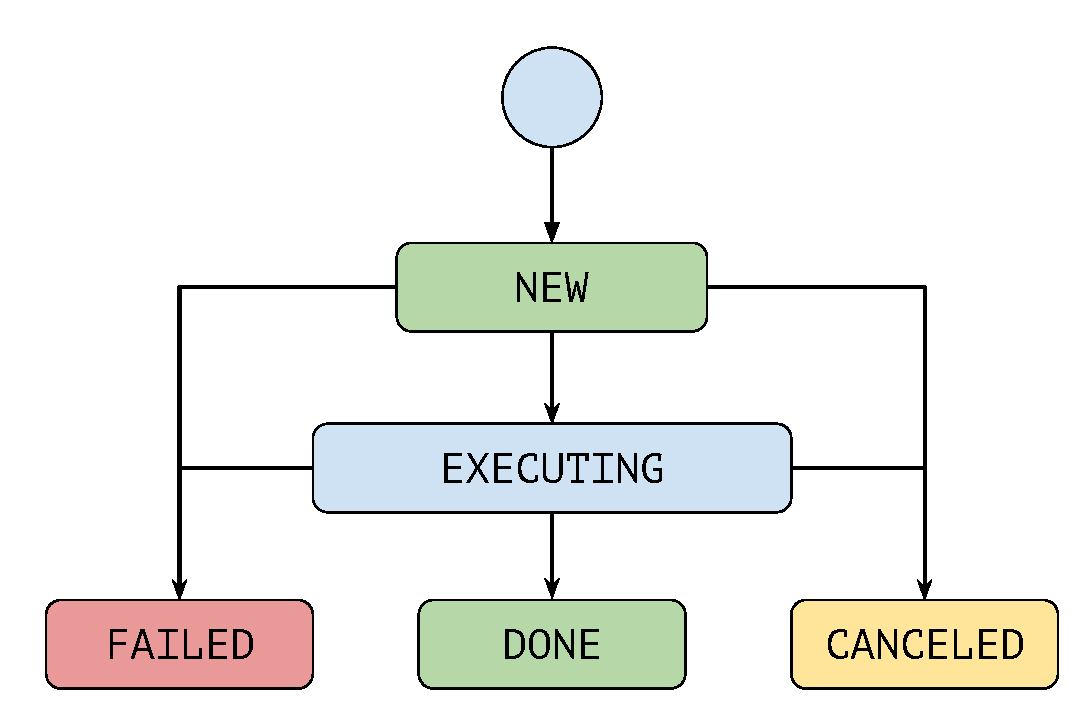
\includegraphics[width=.95\textwidth]{figures/manager/workflow-state-model.pdf}
        \caption{}
        \label{fig:WorkflowStates}
    \end{subfigure}
    \caption{State diagrams for : ~\ref{fig:CampaignStates}) a campaign;~\ref{fig:WorkflowStates}) each workflow of a campaign.}
    \label{fig:StateDiagrams}
\end{figure*}

Similar to the campaign state model, the workflows state model
(Figure~\ref{fig:WorkflowStates}) defines five states: (1) \textit{new}, (2)
\textit{executing}, and (3) \textit{done} or (4) \textit{canceled} or (5)
\textit{failed}. A workflow is in the \textit{new} state when it is received by
the Bookkeeper and transitions to the \textit{executing} state when the Enactor
submits the workflow for execution to the selected WMF. The workflow transitions
to one of the final states---\textit{done}, \textit{canceled} or
\textit{failed}---based on the final state the workflow management system
reports.

The Bookkeeper class defines several methods to execute a campaign. The most
important ones are: \textit{run}, \textit{work} and \textit{monitor}. The
\textit{run} method initializes the campaign state to \textit{new} and sets up
the environment for executing the campaign. \textit{Work} calls the Planner to
produce a plan transitioning the state of the campaign to \textit{planning}.
After a plan is produced, \textit{work} calls \textit{\_verify\_objective} to
verify if the objective of the campaign can be achieved, and either starts
submitting workflows to the Enactor or transitions the campaign to the
\textit{failed} state. In addition, \textit{work} pushes the submitted workflows
to a data structure that the \textit{monitor} method reads. The \textit{monitor}
method checks the state of the workflow which are executing and receives
information from the Enactor via callbacks.

The Planner and Enactor classes define the methods for planning the execution
of a campaign, executing workflows on resource and monitoring their execution.
The Planner defines a \textit{plan} method which implements a planning
algorithm and returns a plan. The Enactor's \textit{enact} method submits a
workflow to the selected WMF. The \textit{monitor} method of the Enactor
checks periodically the state of the workflows that are executing and pushes
state updates to the Bookkeeper via a callback.

\begin{figure*}[t]
    \centering
    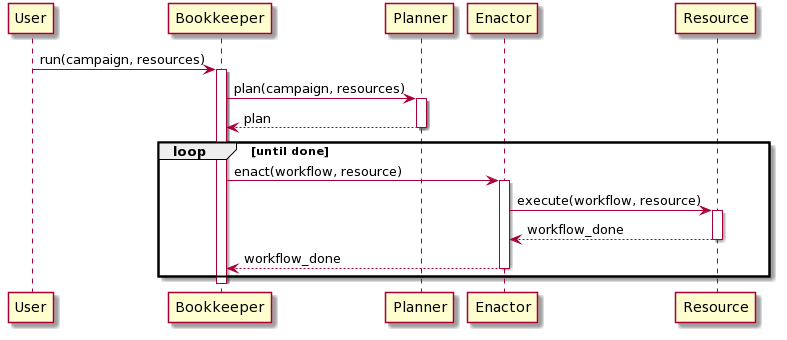
\includegraphics[width=.85\textwidth]{figures/manager/rcm_seq.png}
    \caption{Sequence diagram for executing a computational campaign through the campaign manager prototype}
    \label{fig:seq_diag}
\end{figure*}

Figure~\ref{fig:seq_diag} shows the sequence diagram of the execution. Before
the execution of a campaign, the Bookkeeper gets as input a campaign (a set of
workflows) and a set of resources. As the user requests to execute the campaign,
the Bookkeeper passes to the Planner the information it needs. When the plan is
ready, the execution of the campaign begins with the Bookkeeper passing a
workflow to the Enactor, along with a list of resources to use for the
execution. As the Enactor executes the workflow, it pushes state updates to the
Bookkeeper via callbacks. The Bookkeeper continues to pass workflows to the
Enactor as resources become available, until there are no more workflows to execute.

Instead of an actual workflow management framework (WMF), the Enactor utilizes a
modified version of the workload emulator proposed in
Ref.~\cite{balasubramanian2019programming}. The emulator allows us to define
heterogeneous resources and emulate the execution of workloads on those
resources. A workload is a set of independent tasks that can be executed 
concurrently. We modified the emulator to emulate the execution of a campaign 
which is a set of independent workflows.  In addition, we extended the emulator 
execution capabilities with SimPy~\cite{simpy}, a discrete time simulator. 
SimPy executes discrete simulations by producing events as time progresses. 
These events provide information about which workflows are executing or have 
finished to execute. The Enactor polls these events and pushes to the 
Bookkeeper the state of each workflow. As a result, we are able to simulate the 
execution of a campaign and validate the correctness of our design and its 
implementation.

\begin{figure*}[t]
    \centering
    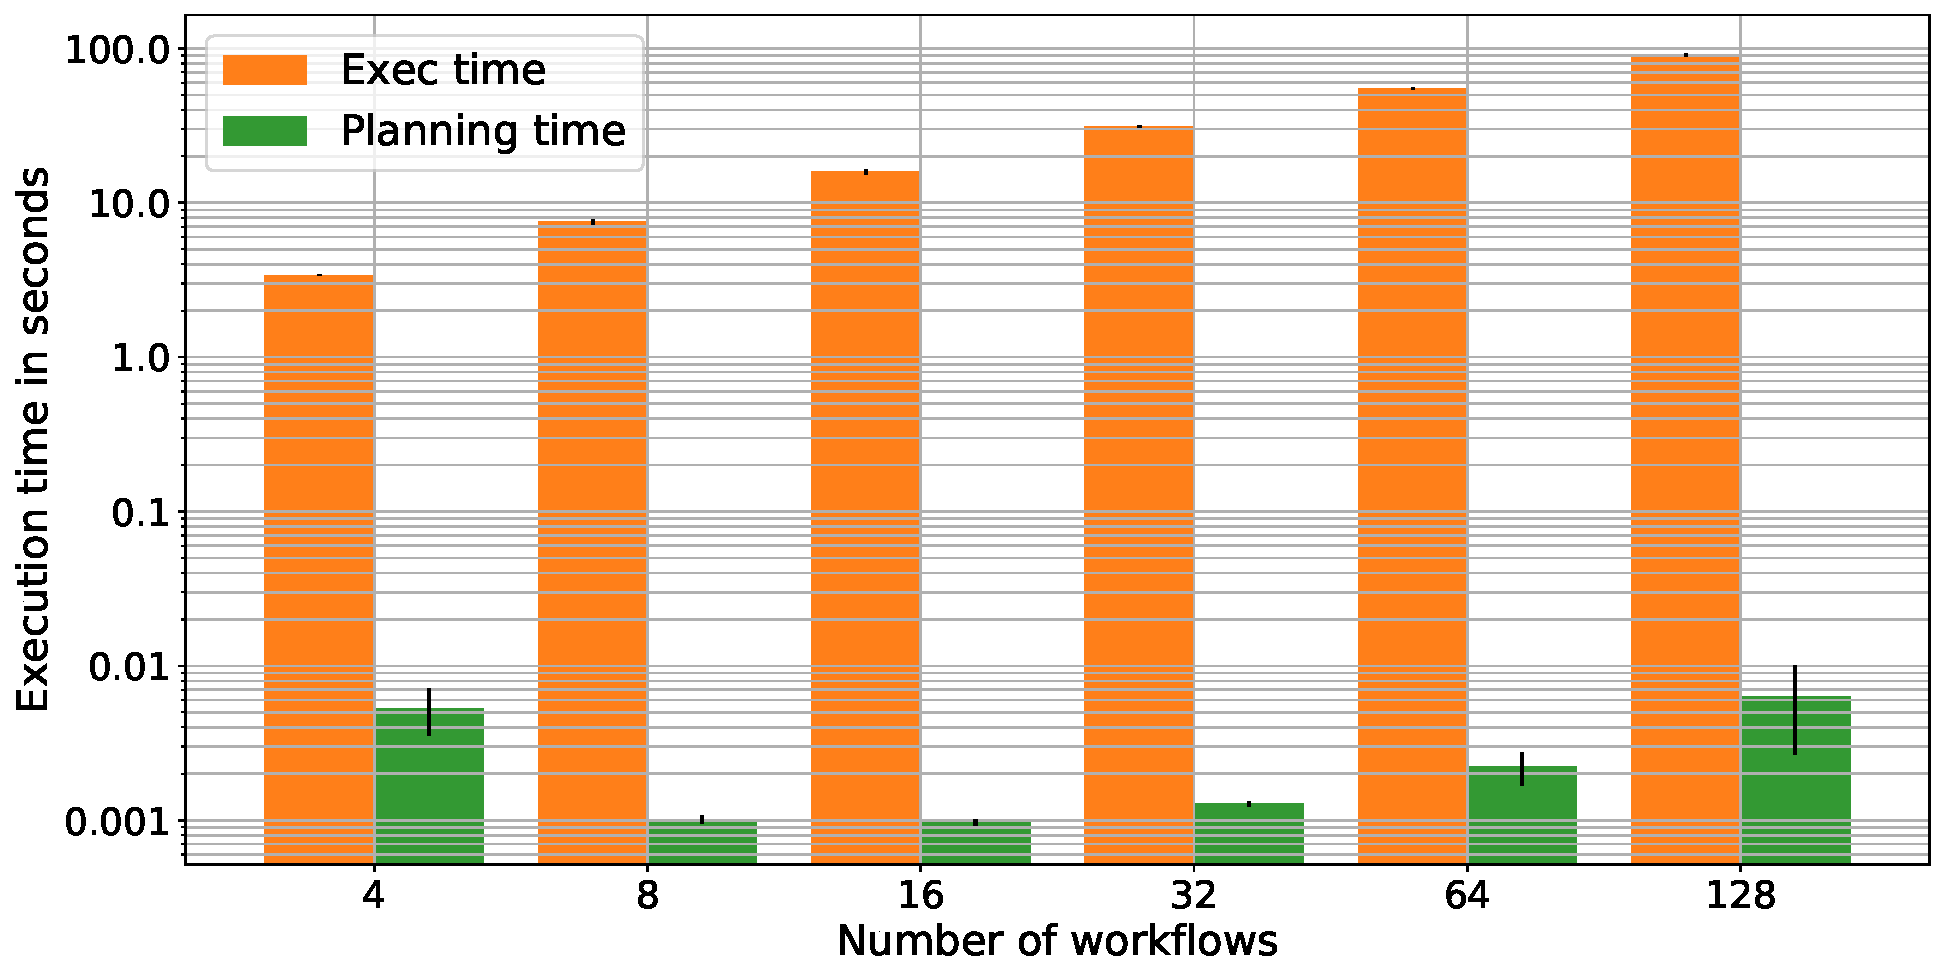
\includegraphics[width=.95\textwidth]{figures/manager/SimTimeWork.pdf}
    \caption{Execution time of simulating the execution of computational campaign with different number of workflows on different number of resources, $N_R$.}
    \label{fig:cm_char}
\end{figure*}

We validated the correctness of our design by executing campaigns of different
sizes on different number of resources. We provided the prototype with a
campaign, a set of resources and an execution plan. We then check that the
workflows of the campaign were executed as expected and in a viable amount of
time, as shown in Figure~\ref{fig:cm_char}. We observed that the execution time
of the simulation increases when more than 64
resources are utilized concurrently. Both the Enactor and the Bookkeeper have
monitoring methods that traverse the list of executing workflows. In
addition, the Enactor uses callbacks to inform the Bookkeeper about the state of
the workflows. Above 64 resources, these operations start to dominate the
execution time of the simulation. The prototype executed 128
workflows on 128 resources in $\approx$15 minutes, an amount of time we considered acceptable for experimental purposes.
% and thus we conclude that this increase will not affect the execution of an
% actual campaign. As a result, we conclude that the design and functionalities
% of the prototype satisfy the requirements and correctly execute a
% computational campaign.


\mtnote{Validation: do the prototype+emulator do what they are supposed to do?
    E.g., given a campaign and an unfeasable amount of resources, do they deem
    the campaign unplannable? Are workflows marked as failed/cancelled as per
    the given specification? Given a feasable amount of resources, do they deem
    the campaign plannable? If you have time/data/tests I would write a
    paragraph along these lines.}

\section{Conclusions}
\label{sec:cm_concl}
In this chapter, we motivated, discussed and validated a prototype for a
software system that supports the execution of computational campaigns on HPC
resources based on a set of use cases. We described the design and the basic
components of the CM, a Bookkeeper, a Planner and an Enactor.
Based on the selected design, we implemented a software prototype that simulates
the execution of a campaign on resources. The prototype allows us to understand
and correctly implement the necessary functionality of the CM.

The CM produces an execution plan for a computational via the Planner class. The
Planner is able to support several planning algorithms. Although using any
planning algorithm would satisfy the requirement of creating an execution plan, 
it is necessary to utilize an algorithm that is able to achieve the campaigns 
objective. In the next chapter, we investigate planning algorithms and evaluate 
the plans they produce for executing computational campaigns.


% ---------------------------------------------------------
% CHAPTER 6
% ---------------------------------------------------------
\chapter{Evaluating Computational Campaigns Planning Algorithms on HPC Platforms}
\label{ch:campaigns}
% !TEX root = main.tex
\label{ch:campaigns}
Computational campaigns enact an execution to achieve a computation objective under given requirements and constraints.
The computational objective is a set of values selected by the user for a set of metrics.
Some of these metrics are time to completion and throughtput.
Furthermore, the objective can be represented as an objective function.
Requirements describe the minimum amount and type of resources needed to execute each workflow of the campaign, while the constrains are the conditions that bound the the execution, such as resource availability, resource capacity or costs.

The objective of a campaign can be translated to a computational objective function that would either minimize or maximize a metric.
Among the many metrics that could be considered, the most common one is the total time taken by a campaign to execute, also known as makespan.
An execution plan of a campaign is a mapping between workflows and resource to execute upon.
Calculating the makespan of a campaign means finding an execution plan that satisfies the computational objective function.

A computational campaign execute on several HPC resources.
These resources are heterogeneous as they offer different type of resources.
One aspect of this heterogeneity is the performance each HPC resources has in terms of Peta-Flops.
In addition, these resources are dynamic as their availability and performance can change over time.

Users have deep knowledge of their workflows and their requirements when they prototype them.
As a result, they may not know accurately the total number of operations of each workflow that comprise their campaign.
This, in turn, makes it even harder to derive an execution plan that will satisfy the objective of the campaign.

We use a campaign from a campaign from a polar science use case to evaluate three classes of planning algorithms.
These classes differ on how they approach the planning problem and in the amount of knowledge they produce to derive a plan.
We experimentally measure and characterize the performance of these classes.

The chapter offers the following contributions:
\begin{inparaenum}[i)]
    \item an experiment-based methodology to compare planning algorithms performance that does not depend on the considered use case and computing framework;
    \item a conceptual framework for selecting planning algorithms based on the algorithm, campaign and resources characteristics
\end{inparaenum}

The chapter is organized as follows: \S~\ref{sec:makespan_calc} discusses the calculation of the makespan of a campaign given a set of assumptions that are progressively relaxed.
Section \S~\ref{sec:algo} discusses three selected makespan calculation algorithms and \S~\ref{sec:algo_perf_comp} compares their performance, i.e the derived makespan.
Finally, section \S~\ref{sec:cf_algo_sel} presents a conceptual framework that will allow users to best select a planning algorithm.

% -------------------------------------------------------------------
\section{Calculating the Makespan of a Campaign}
\label{sec:makespan_calc}
The way workflows of a given campaign are mapped to resources can affect the makespan calculation. 
Figure~\ref{fig:example_makespan} shows an example of a campaign with workflows of different size and execution times, and the makespans that two different mappings produce.
The makespan of the campaign on the left sub~-figure is $20$, while on the right it is $16$.
In addition, the size of the workflows, i.e., the number of resources they require, becomes relevant and resources may be underutilized, as shown in Figure~\ref{fig:example_makespan}.

\begin{figure*}[ht!]
    \centering
    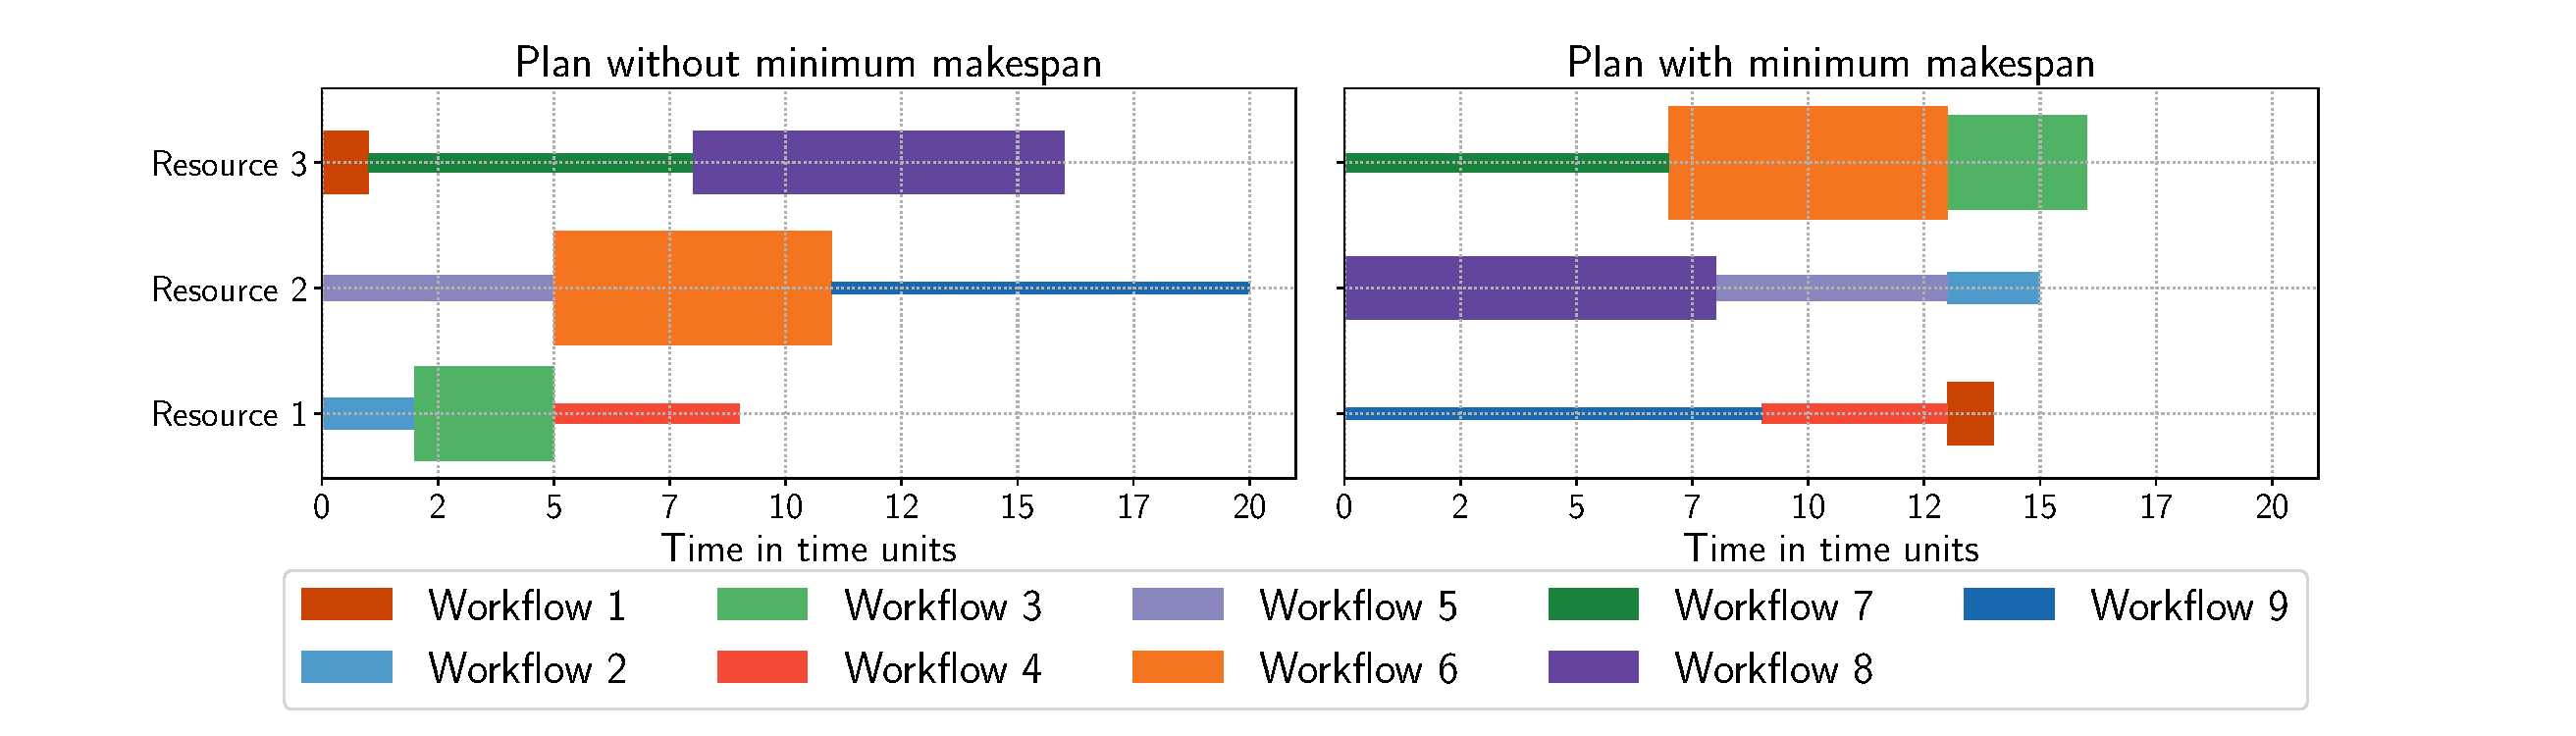
\includegraphics[width=.99\textwidth]{figures/campaign/plan_comp.pdf}
    \caption{Comparison of different campaign execution plans. Based on workflow mapping on resources makespan and resource utilization is different.}\label{fig:example_makespan}
\end{figure*}

We are making a set of assumptions which we do not relax during the initial analysis of a model that calculates the makespan of a campaign.
These are:
\begin{inparaenum}[(1)]
    \item a workflow is an atomic unit and cannot be decomposed;
    \item workflow resource request is sufficient to execute the workflow;
    \item a resource is an aggregate of computing capabilities;
    \item resources are homogeneous;
    \item every workflow of a given campaign can be executed on the given resources;
    \item a random resource selection is based on a uniform distribution;
    \item only one workflow can be executed on a resource at any point in time; and
    \item a workflows can be homogeneous or heterogeneous in space---maximum number of resources they need, and time---the amount of time they are executing.
\end{inparaenum}

We denote a computational campaign as $C = [w_{i}: 1 \leq i \leq N_{C}]$, where $w_{i}$ is a workflow and $N_{C}$ is the total number of workflows, $R = [ r_{j}: 1 \leq j \leq N_{R}]$ is a set of available resources, where $r_{j}$ is a resource and $N_{R}$ is the total number of available resources, and $ M(C,R) = [(w_i, r_j): 1 \leq i \leq N_{C}, r_j \in R] $ is a mapping function of workflows onto resources.
In addition, we denote the execution time of a workflow as $Tx_{w_{i}}$, the makespan of campaign $C$ as $TTX_{C}$, and the makespan of campaign $C$ for a given mapping function $ M $ as $TTX_{C}(M)$.
Assumption~\#3 allows to abstract the resource implementation details, as workflows can be executed on different resources such as HPCs, Clouds, pilots and more. 
Lastly, we will assume homogeneous resources as it simplifies the formalization of the problem.

With a single resource, i.e., $N_{R} = 1$, the workflows of a campaign will be executed sequentially, regardless the execution order or if the workflows are homogeneous or heterogeneous.
As a result the makespan of the campaign is:
\begin{equation}
   TTX_{C} = \sum_{i=1}^{N_{C}}Tx_{w_{i}} 
\end{equation}

With multiple homogeneous resources, i.e., $1 < N_{R} < N_{C}$, the workflows of a campaign can be executed concurrently.
Furthermore, this is semantically equivalent to executing on a single resource large enough to allow concurrent workflow execution, where each workflow executes on a resource partition. 
Because of assumptions~\#5 and~\#7, executing homogeneous or heterogeneous in space workflows has the same makespan.
A random mapping of workflows onto resource will have a makespan:
\begin{equation}
   TTX_{C}(Random) \geq \frac{1}{N_{R}}\sum_{i=1}^{N_{C}} Tx_{w_{i}} 
\end{equation}
Given multiple homogeneous resources, when executing workflows that are heterogeneous in time and that can be homogeneous or heterogeneous in space, the makespan of the campaign for a given mapping function $ M $ is:
\begin{equation}
TTX_{C}(M) = \max_{r_{j}\in R}\Big\{\sum_{w_{i}\in M(C,r_{j})}Tx_{w_{i}}\Big\}
\label{eq:makespan}
\end{equation}

% -------------------------------------------------------------------
\section{Planning Algorithms}
\label{sec:algo}

There is a plethora of methods and algorithms to calculate and optimize the makespan of a workflow~\cite{lu2019review}, including queuing networks~\cite{yao2019throughput,bao2019performance}, domain specific languages~\cite{carothers2017durango,maheshwari2016workflow}, and machine learning~\cite{witt2019predictive,pumma2017runtime}.
From this plethora of selections, we selected to investigate three algorithms, each one representative of a larger family of algorithms.
These are Heterogeneous Earlier Finish Time algorithm (HEFT)~\cite{topcuoglu2002performance}, a genetic algorithm~\cite{page2005algorithm} and a simple heuristic algorithm.

The following sections present the selected algorithms in more detail.
In addition to the algorithmic details, we discuss the knowledge and the information each algorithm produces to derive a plan.
A summary of the algorithms characteristics are shown in Table~\ref{tab:sched_algo}.

\begin{table}[t]
    \centering
    \scriptsize
    \begin{tabular}{@{}ccccc@{}}
        \toprule
        &\textbf{HEFT}     &\textbf{Genetic Algorithm} &\textbf{L2FF} & \textbf{Random} \\
        \midrule
        Decision Policy   &Deterministic &Convergence Criteria &Deterministic& Deterministic\\
        Initial State    &Blank &Semi-random &Blank & Blank\\
        \midrule
        \multicolumn{5}{l}{\textbf{Initial Knowledge}}\\\midrule
        Workflow Operations &Yes & Yes & Yes & No\\
        Resource Performance &Yes &Yes &Yes & No\\
        \midrule
        Produced Knowledge& Resource availability& Resource availability&None&None\\
        \bottomrule
    \end{tabular}
    \caption{Basic characteristics of selected planning algorithms.\label{tab:sched_algo}}
\end{table}

% -------------------------------------------------------------------
\subsection{Heterogeneous Earlier Finish Time (HEFT) algorithm}
\label{algo:heft}
List scheduling algorithms represent a general family of heuristic based scheduling algorithms to schedule workflows described as direct acyclic graphs~\cite{dong2006scheduling,list_sched_wiki}. 
These algorithms assign priorities to tasks based on a heuristic and order them non-increasingly based on the derived priorities.
Then, this list is traversed and tasks are assigned to resources.
HEFT is a classic example of this type of algorithms~\cite{dong2006scheduling}.

HEFT is an offline scheduling algorithm which calculates the makespan of a workflow on heterogeneous resources, in terms of performance.
HEFT has been implemented as part of the planning capabilities in Pegasus~\cite{deelman2015pegasus} and ASKALON~\cite{fahringer2005askalon} amongst other algorithms.
HEFT has been shown to provide better performance in terms of makespan minimization compared to other mapping algorithms~\cite{topcuoglu2002performance,fahringer2005askalon,canon2008comparative}. 

HEFT makes two important assumptions when used on multiple workflows, i.e., a campaign: 
\begin{inparaenum}[(1)] 
    \item any task in a workflow can be executed on all available resources; and 
    \item all resources are always available.
\end{inparaenum}
HEFT is mainly used to derive an execution plan for workflows, i.e., the execution order and resource placement of the tasks that comprise the workflow.
HEFT uses a matrix to represent execution time of tasks on resources, assigning tasks to the resource that minimizes the finish time of the task, and has complexity proportional to the number of dependencies between tasks and the number of resources offered. 
Because we are interested in campaigns, our HEFT extension will provide an execution plan based on workflows as atomic units instead of tasks.
Furthermore, there has been some initial research to extend HEFT to resources that provide CPU and GPUs~\cite{shetti2013optimization}, as well as a HEFT extension on dynamic resources~\cite{dong2007pfas}. 
Algorithm~\ref{alg:heft} shows HEFT for placing independent heterogeneous workflows on heterogeneous resources.

\begin{algorithm}[ht]
    \caption{Heterogeneous Earliest Finish Time (HEFT) algorithm}
    \label{alg:heft}
    \begin{algorithmic}[1]
        \Procedure{HEFT}{$W$,$R$}\Comment{$W$ and $R$ are a set of workflow and resources respectively}
        \State \texttt{Calculate the computation cost $w_{tx}^{ij}$ of each workflow for all resources}
        \State \texttt{Assign $rank_i = \overline{w_{i}} = \nicefrac{\sum_{j=1}^{|R|}w_{tx}^{ij}}{|R|}$}
        \State \texttt{Sort workflows by non-increasing order of $rank_i$}
        \While{unscheduled workflows}
        \State \texttt{Select the first workflow $\tilde{w}$ from the sorted list}
        \For{$\forall r_{j}$ in $R$}
        \State\texttt{Compute earliest finish time for $\tilde{w}$ on $r_{j}$, $eft_{\tilde{w},r_j}$ }
        \EndFor
        \State \texttt{Assign  $\tilde{w}$ on $r_k$ with $\min{(eft_{\tilde{w},r_j})}$}
        \EndWhile
        \EndProcedure
    \end{algorithmic}
\end{algorithm}

As mentioned above HEFT makes the assumption that all resources are always available and static.
Based on this assumption, HEFT makes the implicit assumption that resources are available based on the times it internally computes.
As a result, it has no external knowledge or representation of when a resource becomes available.
HPC resources may become unavailable for multiple reasons, including but not limited to maintenance, a random failure, executing a workflows over the expected time., etc.
In order to be able to utilize HEFT for dynamic resources, we had to extend Algorithm~\ref{alg:heft} to take as input the time that a resource is initially available.
This input can be represented as a dictionary where the keys are the available resources and the values are the time a resource becomes available.
The extended algorithm is shown in Algorithm~\ref{alg:ext_heft}.
Although the extension may be small, it is crucial to allow to reuse HEFT based on the state of the execution at a given point in time.

\begin{algorithm}[ht]
    \caption{Extended Heterogeneous Earliest Finish Time (EHEFT) algorithm}
    \label{alg:ext_heft}
    \begin{algorithmic}[1]
        \Procedure{EHEFT}{$W$, $R$, $T$}\Comment{$W$ and $R$ are a set of workflow and resources respectively. $T$ is a dictionary of when a resource becomes available.}
        \State \texttt{Calculate the computation cost $w_{tx}^{ij}$ of each workflow for all resources}
        \State \texttt{Assign $rank_i = \overline{w_{i}} = \nicefrac{\sum_{j=1}^{|R|}w_{tx}^{ij}}{|R|}$}
        \State \texttt{Sort workflows by non-increasing order of $rank_i$}
        \While{unscheduled workflows}
        \State \texttt{Select the first workflow $\tilde{w}$ from the sorted list}
        \For{$\forall r_{j}$ in $R$}
        \State\texttt{Compute earliest finish time for $\tilde{w}$ on $r_{j}$ based on $T(r_j)$, $eft_{\tilde{w},r_j}$ }
        \EndFor
        \State \texttt{Assign  $\tilde{w}$ on $r_k$ with $\min{(eft_{\tilde{w},r_j})}$}
        \EndWhile
        \EndProcedure
    \end{algorithmic}
\end{algorithm}

% -------------------------------------------------------------------
\subsection{Genetic Algorithm}
\label{algo:gen}
Genetic algorithms are represent another family of algorithms that are been used to minimize the makespan of an execution~\cite{dong2006scheduling}.
Genetic algorithms are evolving to the final answer as they iterate and improve possible answers.
In general, genetic algorithms are working based on the following procedure:
\begin{inparaenum}[(i)]
    \item create an initial population, where the population is a set of chromosomes. 
          Chromosomes, in the context of planning the execution workflows on resources, is a potential placement of workflows on resources;
    \item evaluate the chromosomes based on a fitness value, which represents the makespan on the campaign;
    \item reproduce by selecting chromosomes, either randomly or based on their fitness value, and generate a new set of chromosomes (called children);
    \item mutate randomly, where randomly selected workflows from a random chromosome are reassigned to resources; and
    \item re-evaluate chromosomes in the population to check convergence.
\end{inparaenum}

The selected genetic algorithm~\cite{page2005algorithm} is developed to support the placement of independent task on heterogeneous resources.
It assumes that all tasks can be executed on all available resources, are independent and indivisible.
These assumptions are in accordance with the assumptions made for workflows in a campaign.
As a result, this algorithm can be extended to support scientific campaigns.
The pseudocode of this algorithm is shown in Algorithm~\ref{alg:gen_algo}.

\begin{algorithm}[ht]
    \caption{Genetic Algorithm}
    \label{alg:gen_algo}
    \begin{algorithmic}[1]
        \Procedure{GA}{$W$, $R$, $T$}\Comment{$W$ and $R$ are a set of workflow and resources respectively. $T$ is a dictionary of when a resource becomes available.}
        \State \texttt{Initaliaze population}
        \While{Conergence Criteria not met and \#Gen $<$ Total\_Generations}
        \State{Selection}
        \State{Reproduce}
        \State{Randomly mutate}
        \State{Balance}
        \EndWhile
        \EndProcedure
    \end{algorithmic}
\end{algorithm}

The chromosomes of the initial population are constructed semi-random.
Specifically, a specific percentage of the workflows are assigned randomly to resources, where the assignment is drawn by uniform distribution.
The rest of the workflows are assigned based on an earlier finish time (EFT) heuristic, similar to the one used by HEFT.
The population size is relatively small to 20 chromosomes, i.e., potential plans, called micro-GA.
Micro-GA reduces the computational load of the genetic algorithm, while it does not significantly impact the final result~\cite{zomaya2001observations}.

Selection of the chromosomes to reproduce is based on a fitness function, which calculates the relative distance from a theoretical optimal processing time.
Each chromosome is assigned a fitness value, which then defines the probability of a chromosome to be selected.
Reproduction uses cyclic rotation to generate the new population members.
Mutation randomly selects an individual from the population and randomly swaps workflows.
Finally, a rebalancing heuristic tries to rebalance and create fitter individuals in the population.

We extend this algorithm in the population initialization to support replanning..
The initialization method takes into account the times resources will be available during for the EFT heuristic.
Another point of extension would be the fitness function.
However, the fitness function of the selected algorithm~\cite{page2005algorithm} already takes into account the previous load of a resource, which is the time a resource is available.

% -------------------------------------------------------------------
\subsection{Longest to Fastest First Available Resource Algorithm}
\label{algo:l2ff}
The last algorithm places workflows based on the rule largest workflows to fastest resource~\cite{balasubramanian2019programming}.
This algorithm sorts the workflows based on the number of operations and resources based on their performance.
Then it places each workflow on the first fastest available resource.
Algorithm~\ref{alg:l2ff} show the pseudocode for this algorithm.

\begin{algorithm}[ht]
    \caption{Longest to Fastest First (L2FF)}
    \label{alg:l2ff}
    \begin{algorithmic}[1]
        \Procedure{l2ff}{$W$, $R$}\Comment{$W$ and $R$ are a set of workflow and resources respectively.}
        \State \texttt{$W_{sorted}=sort(W)$} 
        \State \texttt{$R_{sorted}=sort(R)$}
        \For{$w$ in $W_{sorted}$}
        \State{Assign $w$ to $r_{k}$ where $k=w_{idx} \mod N_{R}$}
        \EndFor
        \EndProcedure
    \end{algorithmic}
\end{algorithm}

This algorithm does not specify in any way when resources are either becoming or are available.
As a consequence, there is no need to extend it when dynamic resources are used, as long as the resource performance is updated accordingly.

% -------------------------------------------------------------------
\section{Performance Evaluation of Planning Algorithms}
\label{sec:algo_perf_comp}

We executed two experiments in order to analyze the performance of the selected planners in terms of the makespan they produce.
In addition to these two experiments, we also executed an experiment to measure the time each planner took to provide a plan.
These sets of experiments allows us to a methodology to compare planning algorithms and decide which algorithm is more suited based on a campaign's computation requirements, i.e. workflow size and resource performance/availability.

\subsection{Experiment 1: Measuring  makespan on static resources}

- Analysis of homogeneous/homogeneous cases:

\begin{figure*}[ht!]
    \centering
    \begin{subfigure}[b]{0.45\textwidth}
        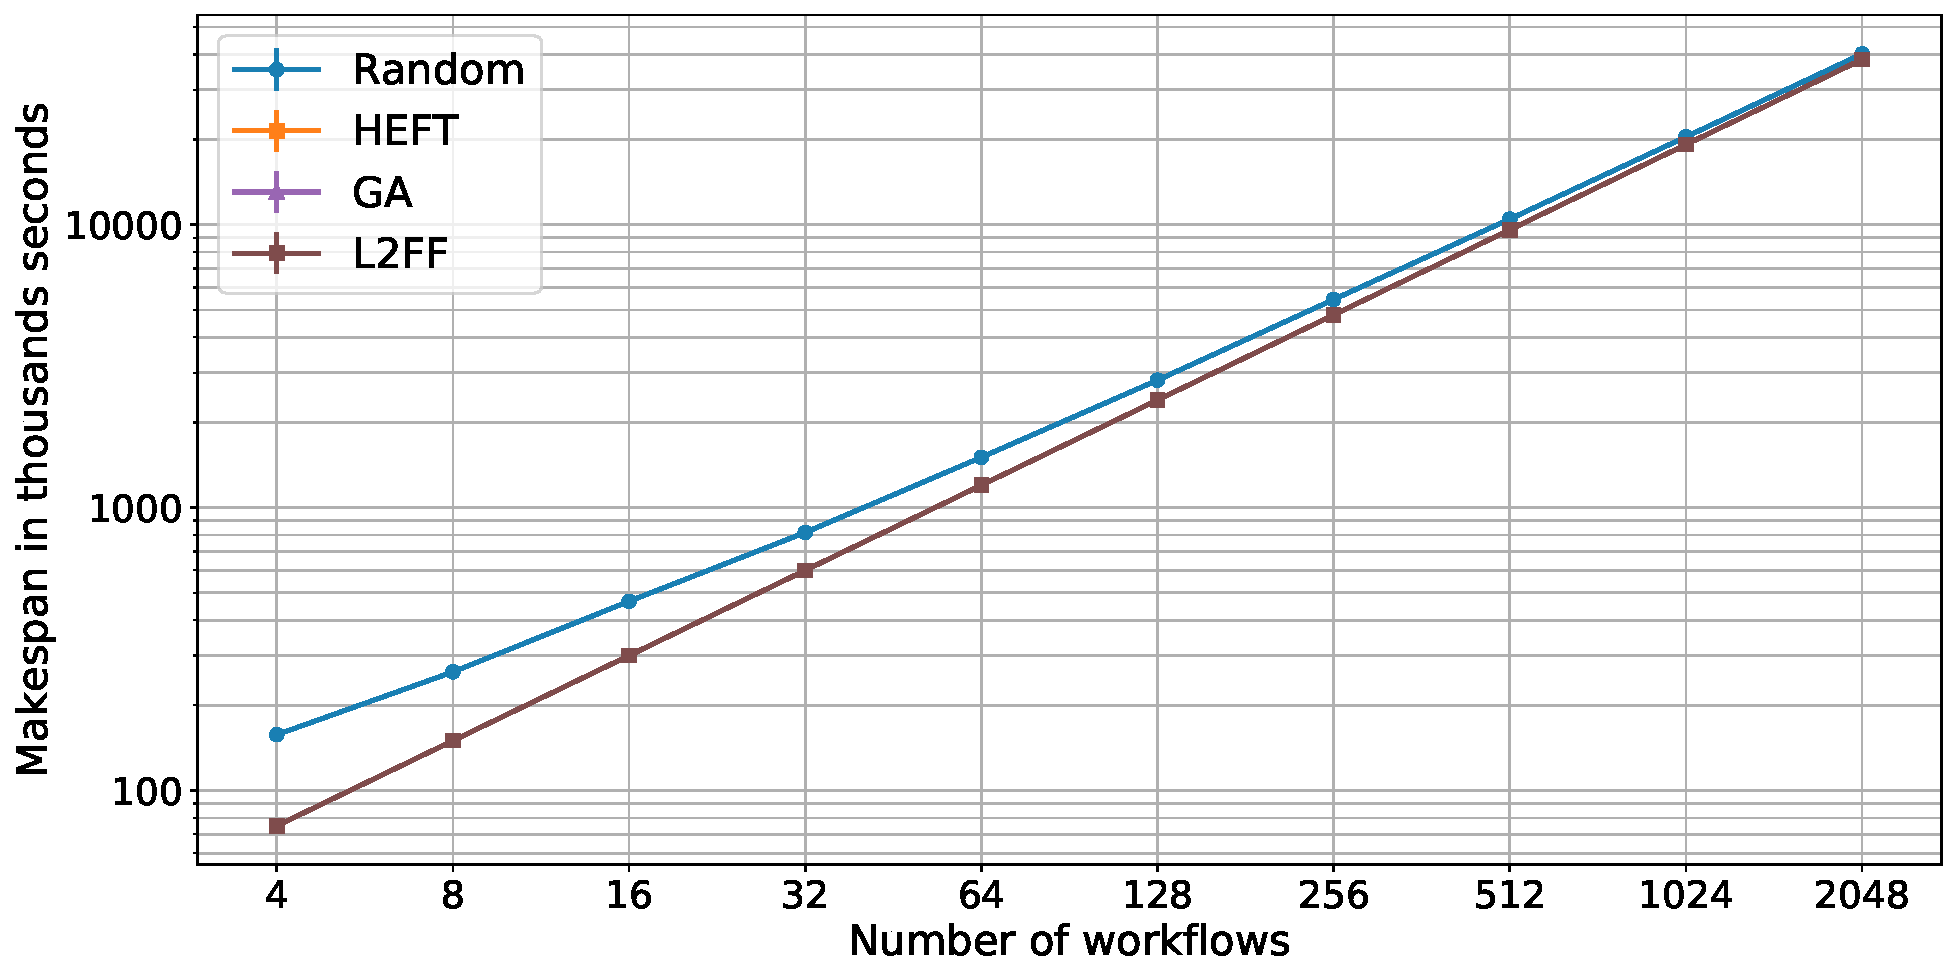
\includegraphics[width=.95\textwidth]{figures/campaign/StHomoCampaigns_4StHomoResources.pdf}
        \caption{}
        \label{fig:StHomoCampaigns_4StHomoResources}
    \end{subfigure}%
    ~ 
    \begin{subfigure}[b]{0.45\textwidth}
        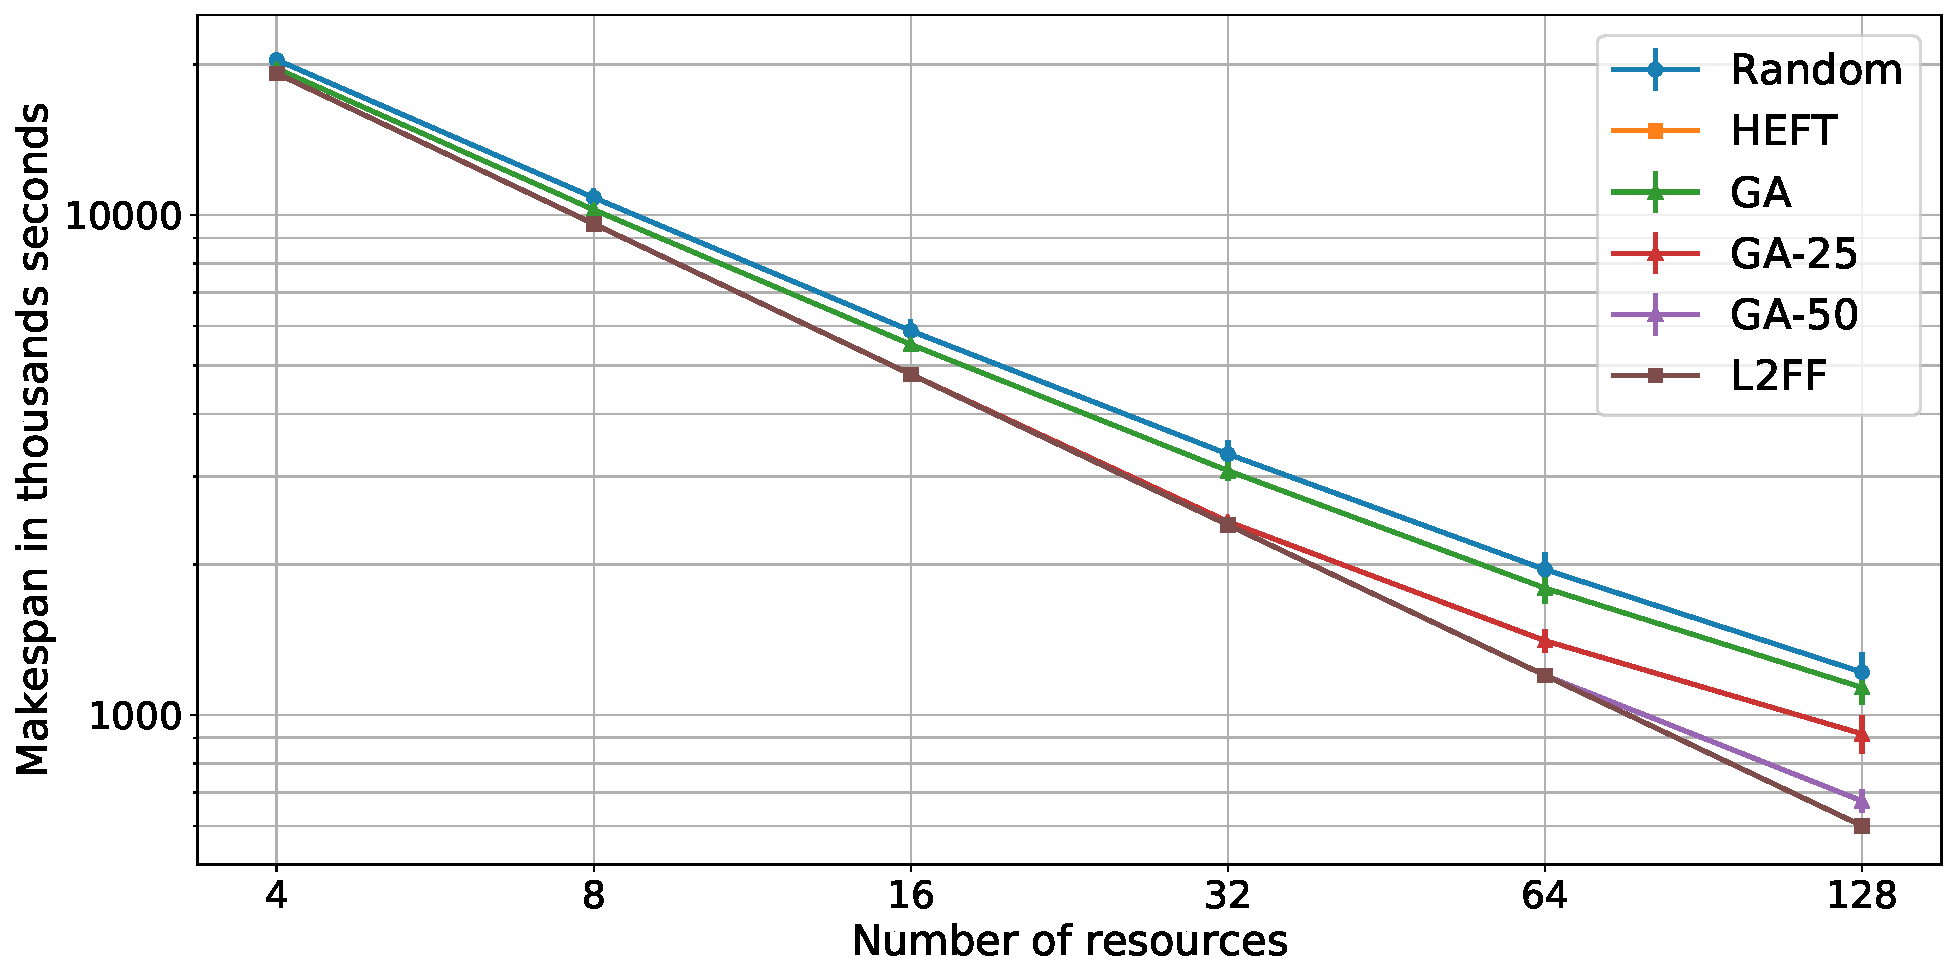
\includegraphics[width=\linewidth]{figures/campaign/StHomoResources_StHomoCampaigns.pdf}
        \caption{}
        \label{fig:StHomoResources_StHomoCampaigns}
    \end{subfigure}
    \caption{~\ref{fig:StHomoCampaigns_4StHomoResources} Makespan of increasing number of homogeneous worklfows on homogeneous resources.
    ~\ref{fig:StHomoResources_StHomoCampaigns} Makespan of homogeneous campaign on different number of homogeneous resources.}
    \label{fig:dyn_homog_analysis}
\end{figure*}



\begin{figure*}[ht!]
    \centering
    \begin{subfigure}[b]{0.45\textwidth}
        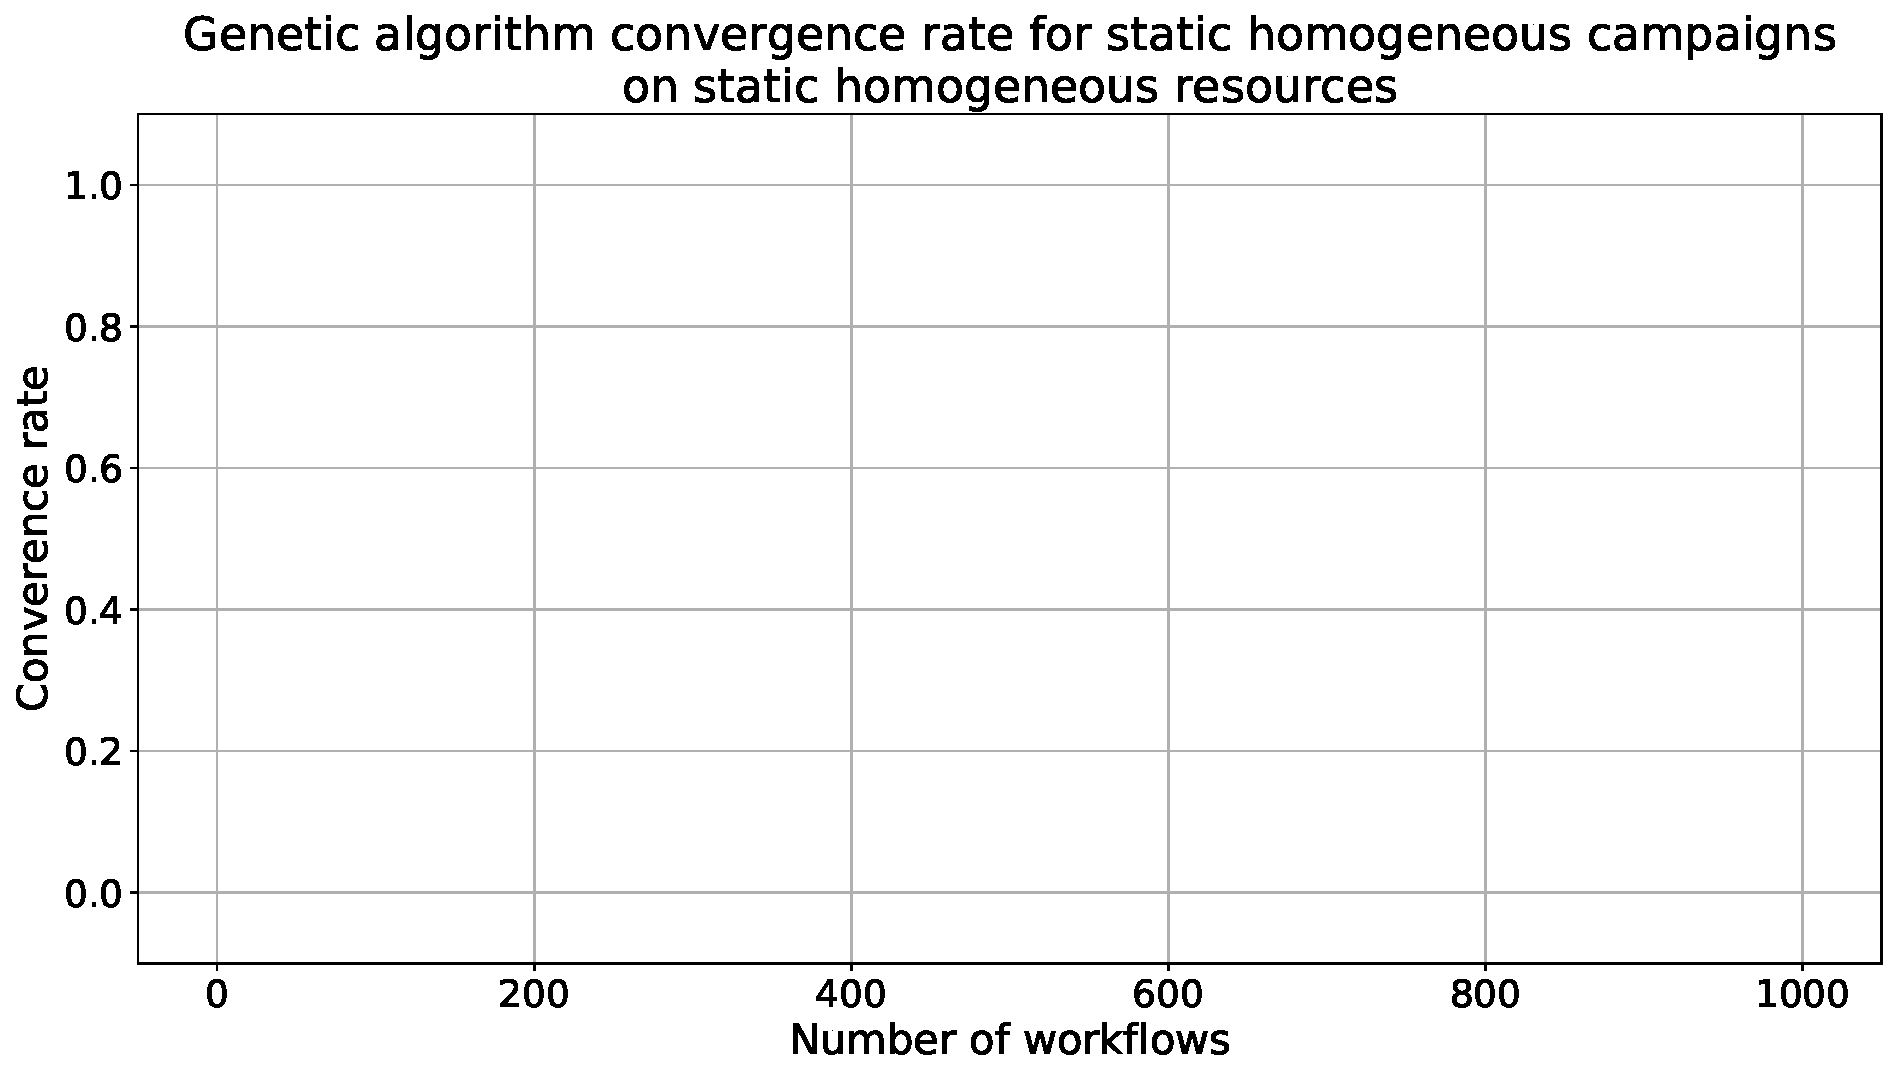
\includegraphics[width=.95\textwidth]{figures/campaign/GAconv_StHomoCampaigns_4StHomoResources.pdf}
        \caption{}
        \label{fig:ga_conv1}
    \end{subfigure}%
    ~ 
    \begin{subfigure}[b]{0.45\textwidth}
        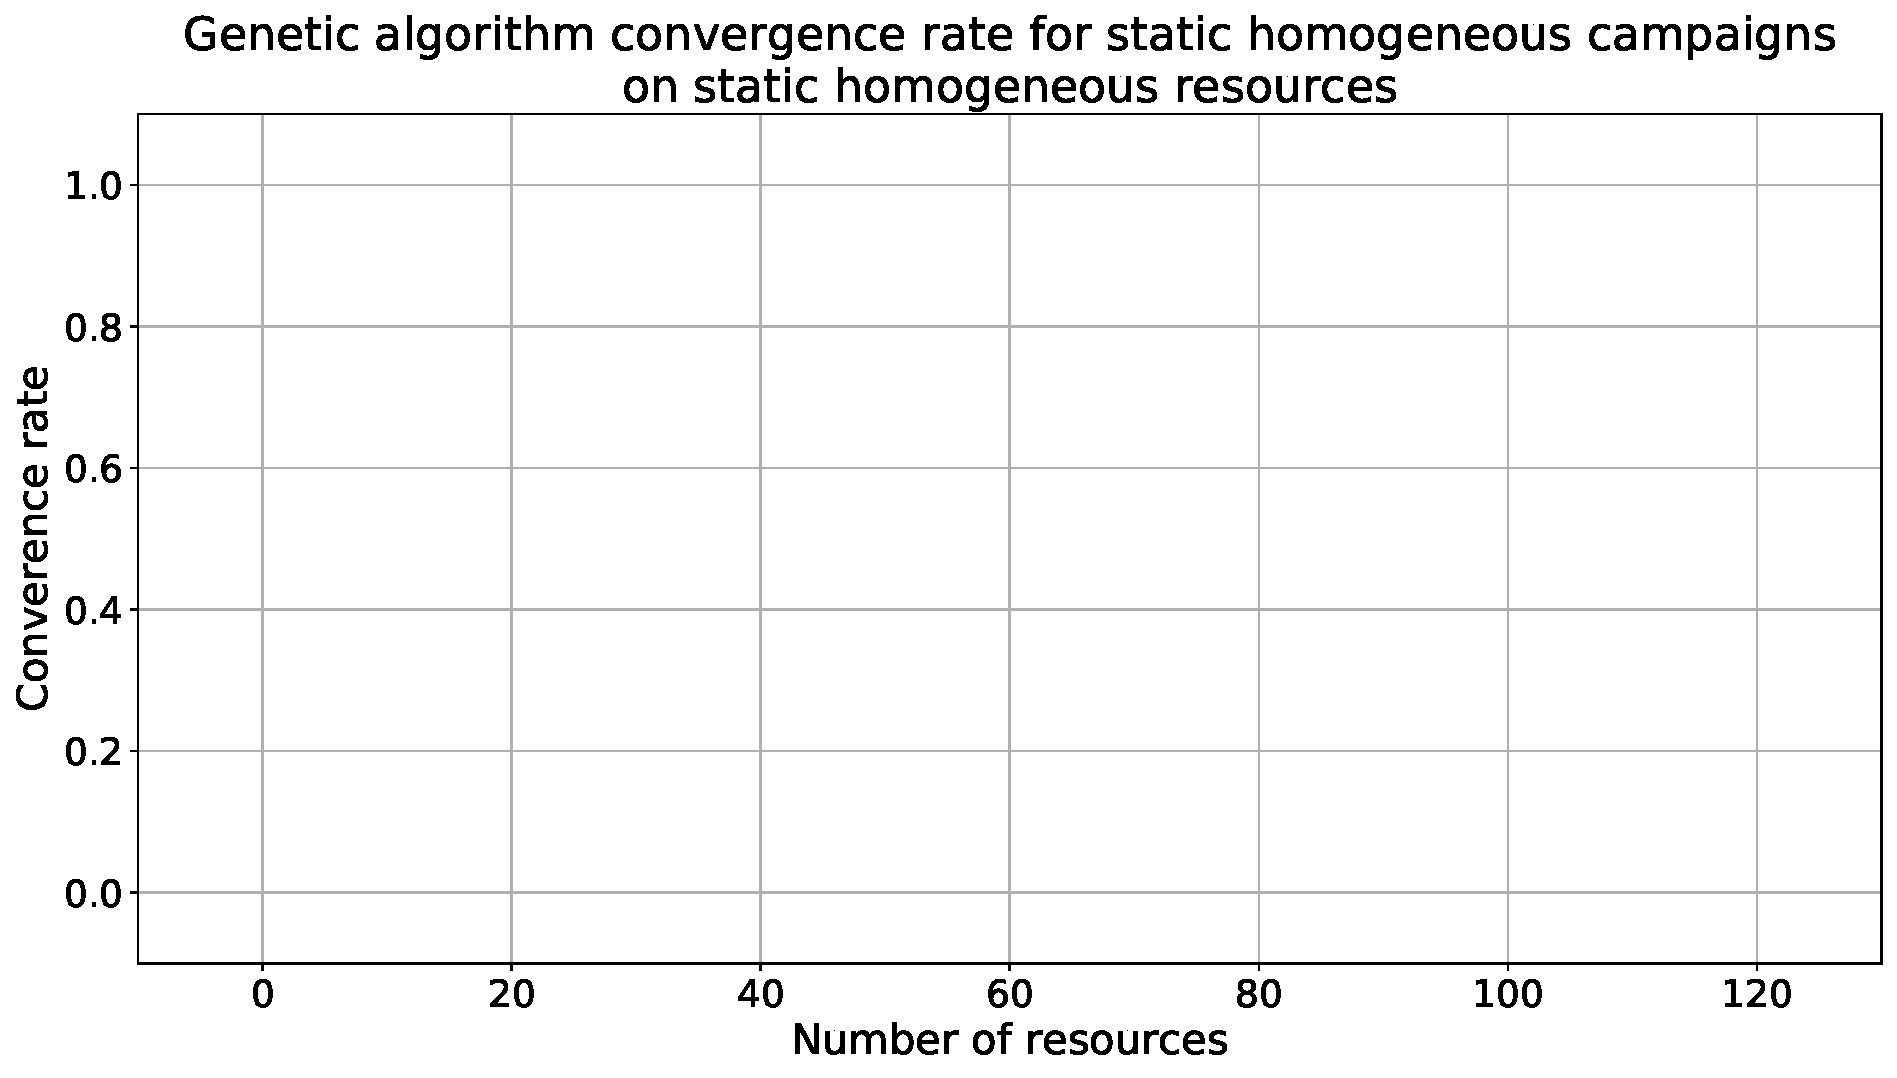
\includegraphics[width=\linewidth]{figures/campaign/GAconv_StHomoResources_StHomoCampaigns.pdf}
        \caption{}
        \label{fig:ga_conv2}
    \end{subfigure}
    \caption{Convergence rate of Genetic algorithm for homogeneous campaigns on static homogeneous resources based on random initialization percentage: ~\ref{fig:ga_conv1}) Different campaign sizes on 4 resources;~\ref{fig:ga_conv2}) Campaign with 1024 workflows and different number of resources.}
    \label{fig:conv_rate}
\end{figure*}

- Analysis of heterogeneous/heterogeneous cases:

\begin{figure*}[ht!]
    \centering
    \begin{subfigure}[b]{0.45\textwidth}
        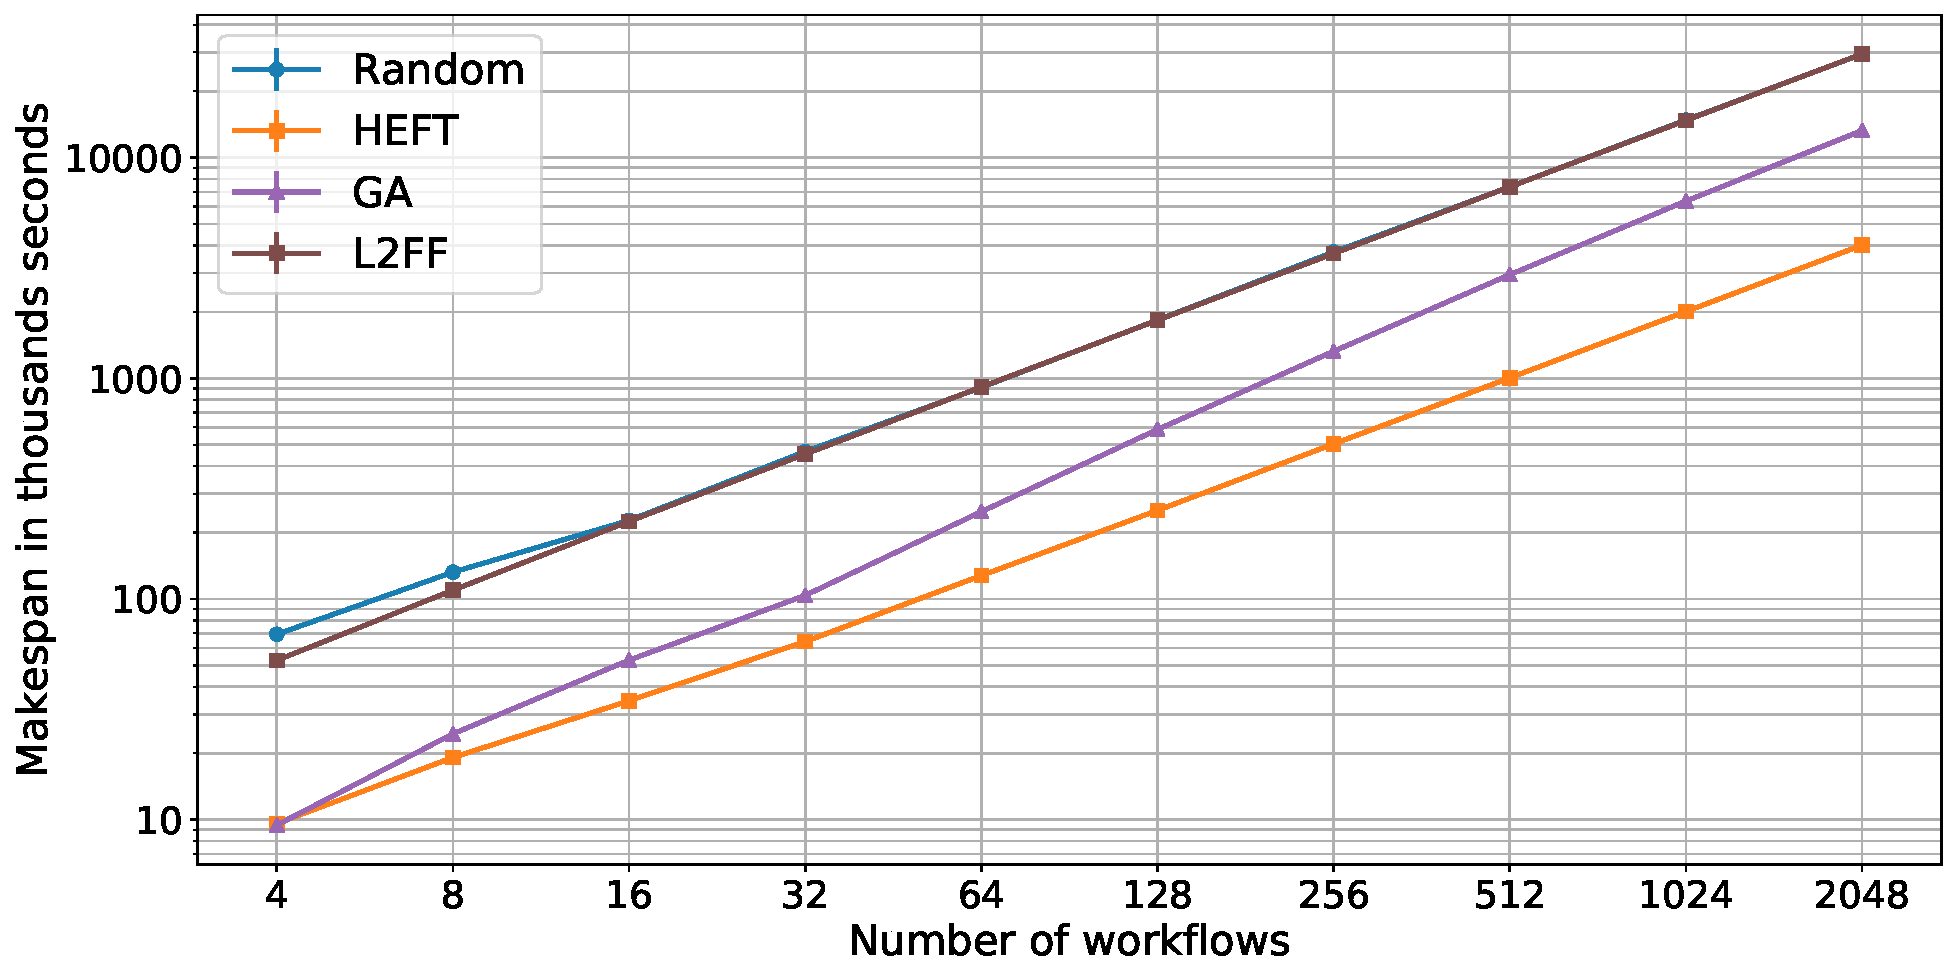
\includegraphics[width=.95\textwidth]{figures/campaign/StHeteroCampaigns_4StHeteroResources.pdf}
        \caption{}
        \label{fig:StHeteroCampaigns_4StHeteroResources}
    \end{subfigure}%
    ~ 
    \begin{subfigure}[b]{0.45\textwidth}
        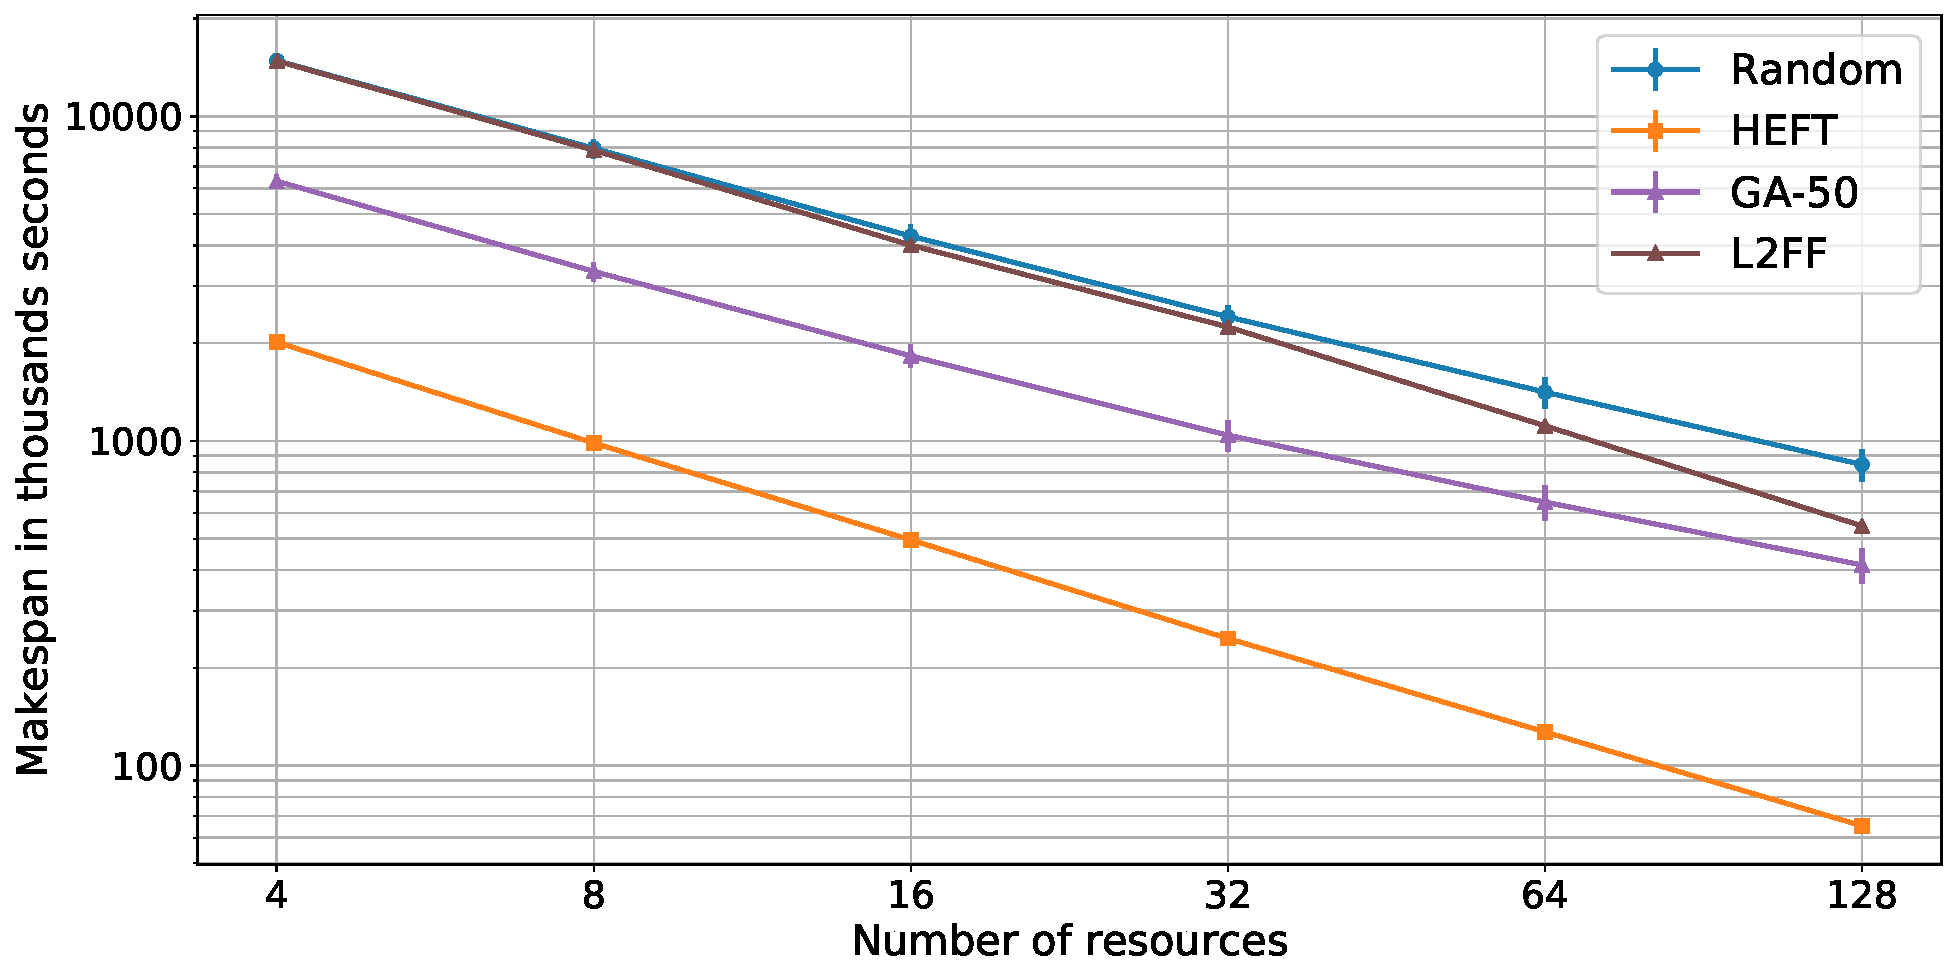
\includegraphics[width=\linewidth]{figures/campaign/StHeteroResources_StHeteroCampaigns.pdf}
        \caption{}
        \label{fig:StHeteroResources_StHeteroCampaigns}
    \end{subfigure}
    \caption{~\ref{fig:StHeteroCampaigns_4StHeteroResources}) Makespan of increasing number of heterogeneous worklfows on heterogeneous resources;
        ~\ref{fig:StHeteroResources_StHeteroCampaigns}) Makespan of heterogeneous campaign on different number of heterogeneous resources..}
    \label{fig:heter_analysis}
\end{figure*}

Generally on Static resources, HEFT provides consistently the best makespan compared to the other algorithms.
This is because: 1) its deterministic behavior, as it produce always the same plan for the same workflows and resources; and 2) its knowledge of when a resource is available.
The genetic algorithm provides worse makespan compared to HEFT mainly because of the randomness introduced during the population initialization.

\subsection{Experiment 2: Measuring makespan on dynamic resources}

- Analysis of homogeneous/homogeneous cases: Resource dynamism is drawn by a normal distribution.

We calculate the final makespan based on the plan that was offered initially.
 I expect that HEFT will be better than other planners, with the genetic and the L2FF being very close to random.
\begin{figure*}[ht!]
    \centering
    \begin{subfigure}[b]{0.45\textwidth}
        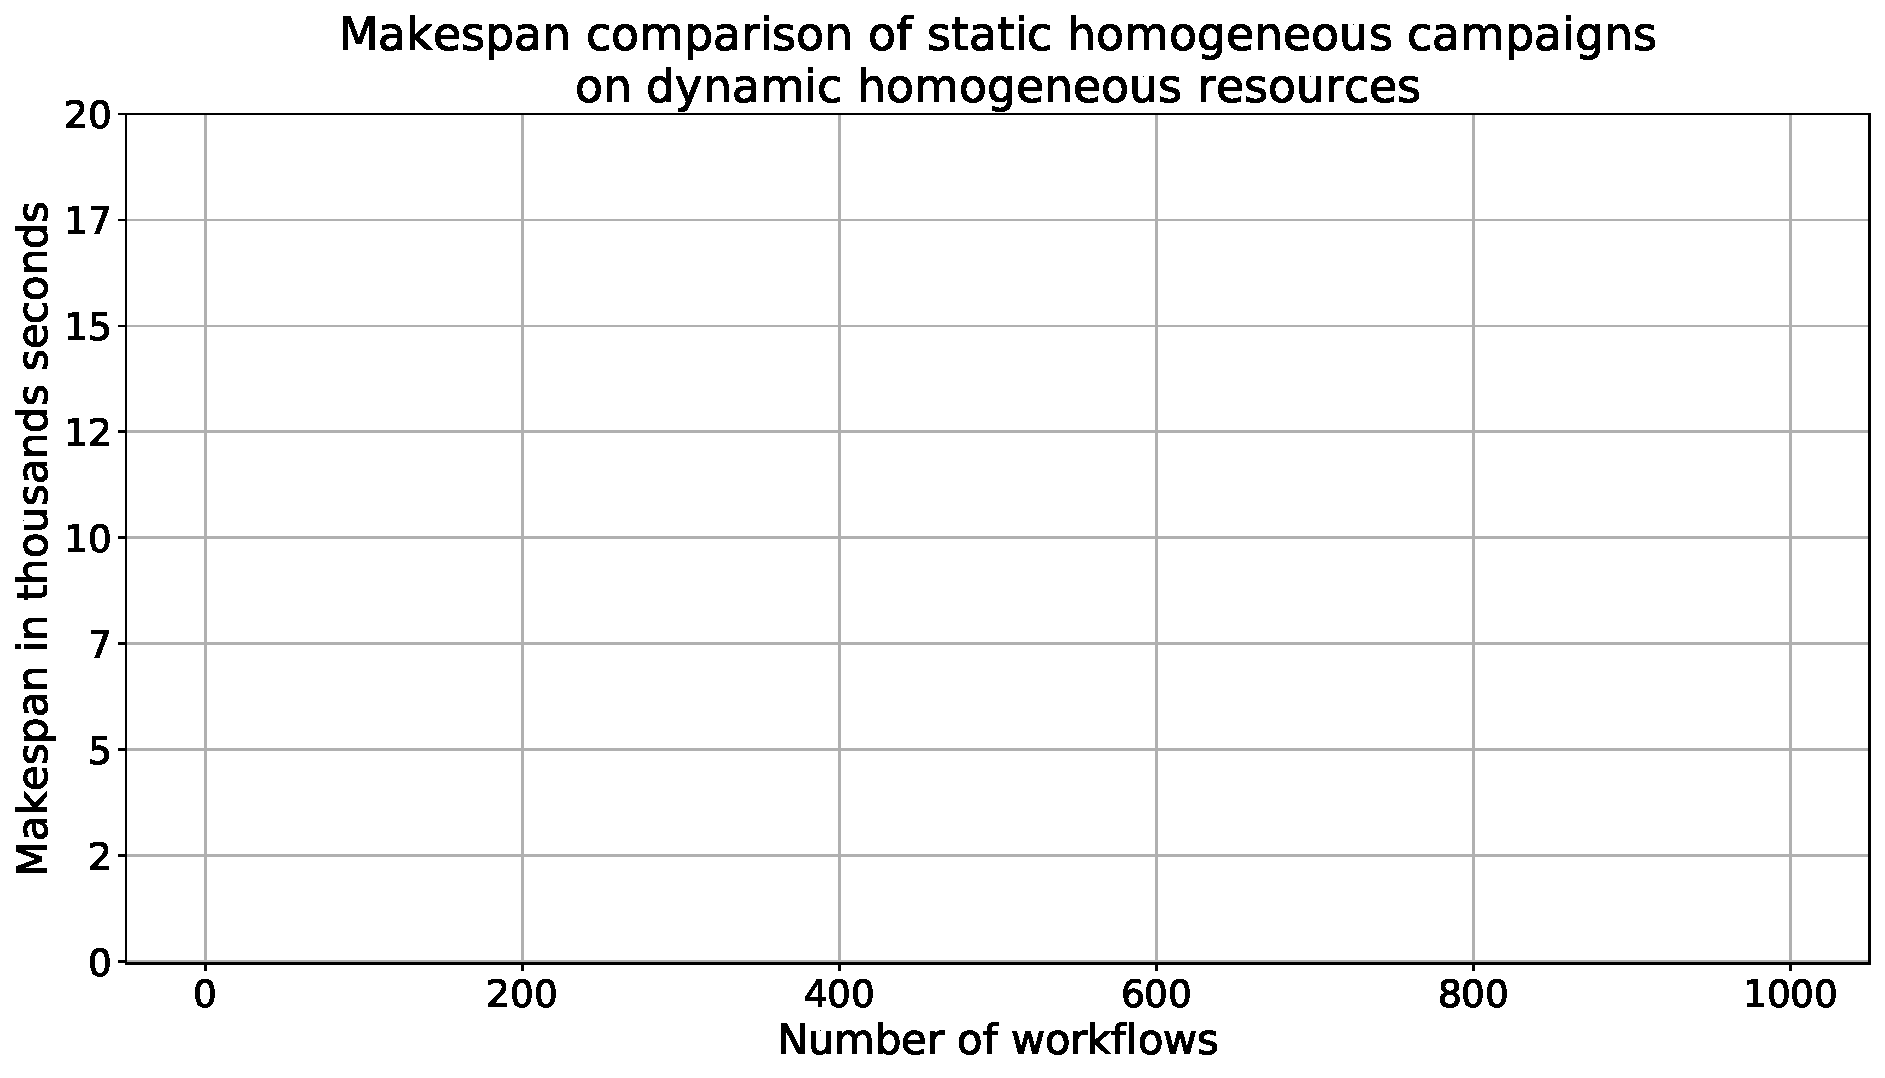
\includegraphics[width=.95\textwidth]{figures/campaign/StHomoCampaigns_4DyHomoResources.pdf}
        \caption{}
        \label{fig:StHomoCampaigns_4DyHomoResources}
    \end{subfigure}%
    ~ 
    \begin{subfigure}[b]{0.45\textwidth}
        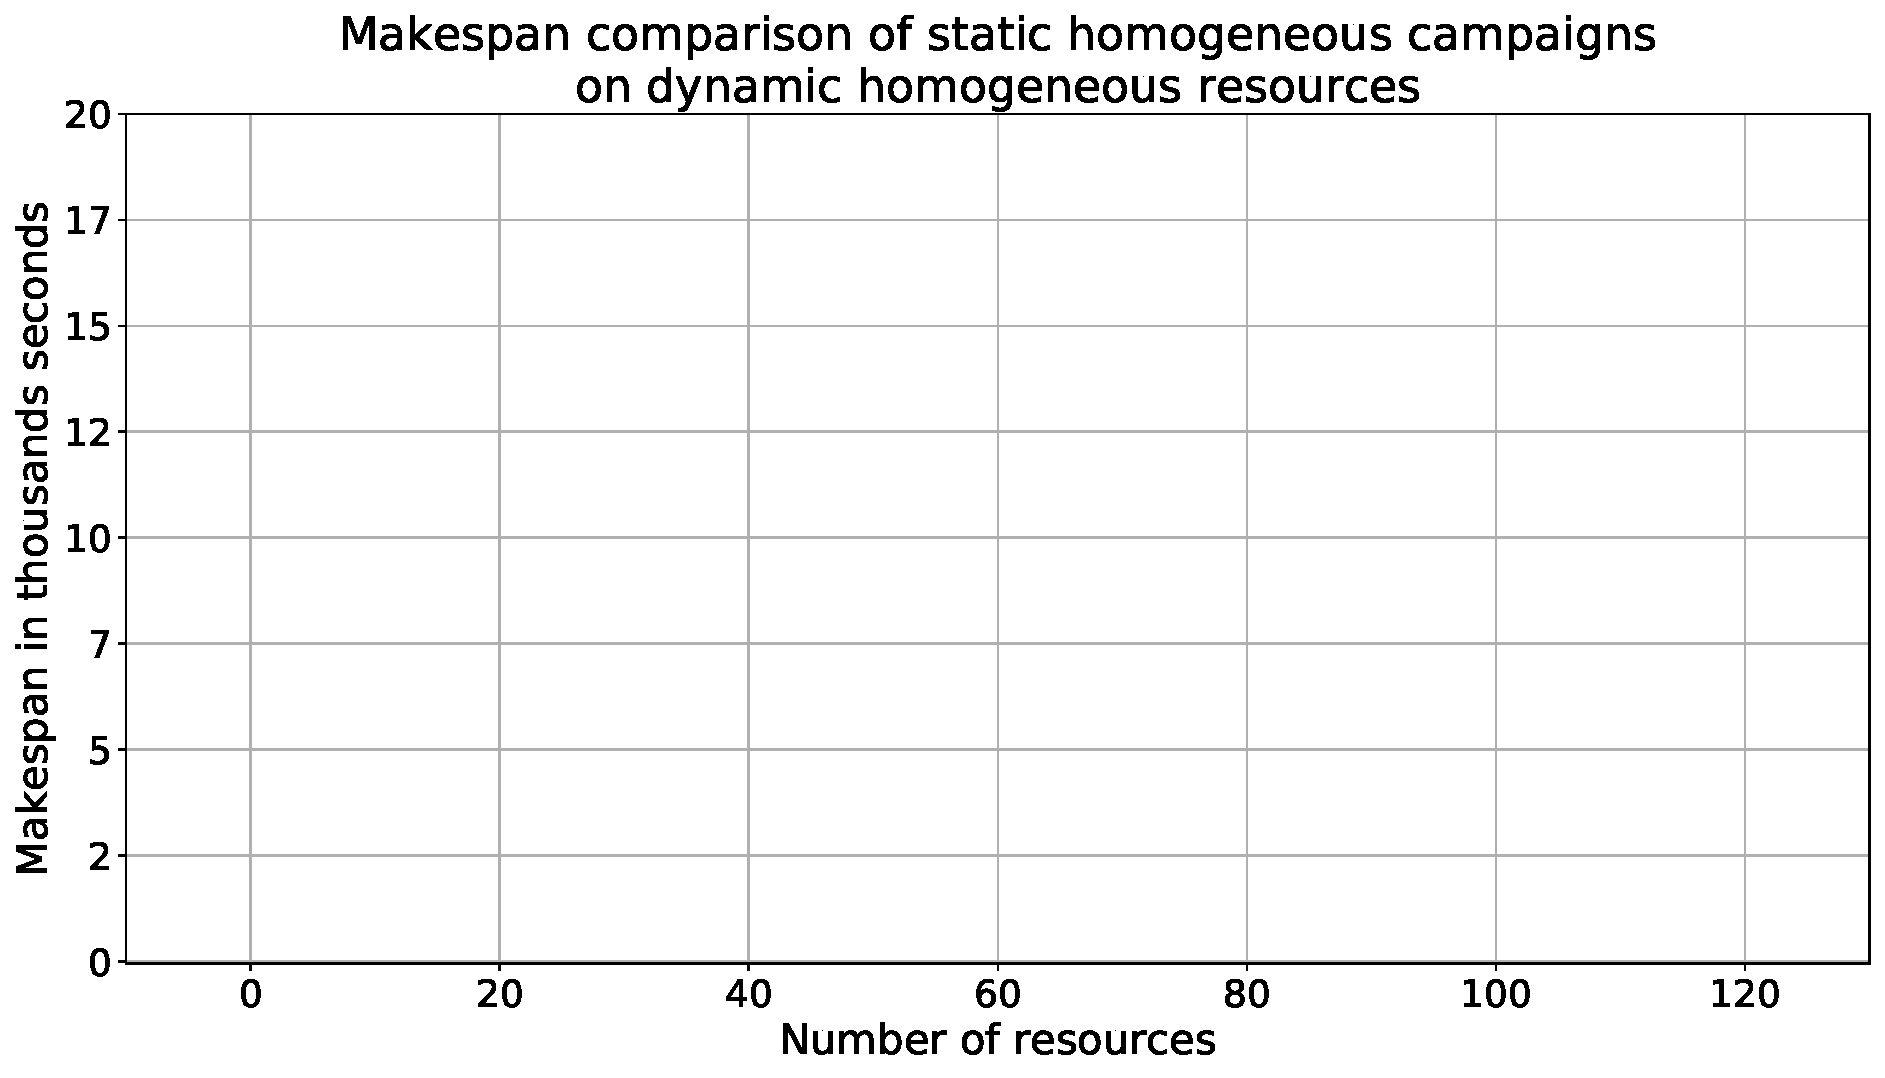
\includegraphics[width=\linewidth]{figures/campaign/DyHomoResources_StHomoCampaigns.pdf}
        \caption{}
        \label{fig:DyHomoResources_StHomoCampaigns}
    \end{subfigure}
    \caption{~\ref{fig:StHomoCampaigns_4DyHomoResources} Makespan of increasing number of homogeneous workflows on homogeneous resources;
        ~\ref{fig:DyHomoResources_StHomoCampaigns} Makespan of homogeneous campaign on different number of homogeneous resources.}
    \label{fig:no_replan_homog_analysis}
\end{figure*}


- Analysis of heterogeneous/heterogeneous cases:
I do not expect significant differences between planners.
I think that the final makespan will be similar for all planners and the will not be distinguishable within error bars.
\begin{figure*}[ht!]
    \centering
    \begin{subfigure}[b]{0.45\textwidth}
        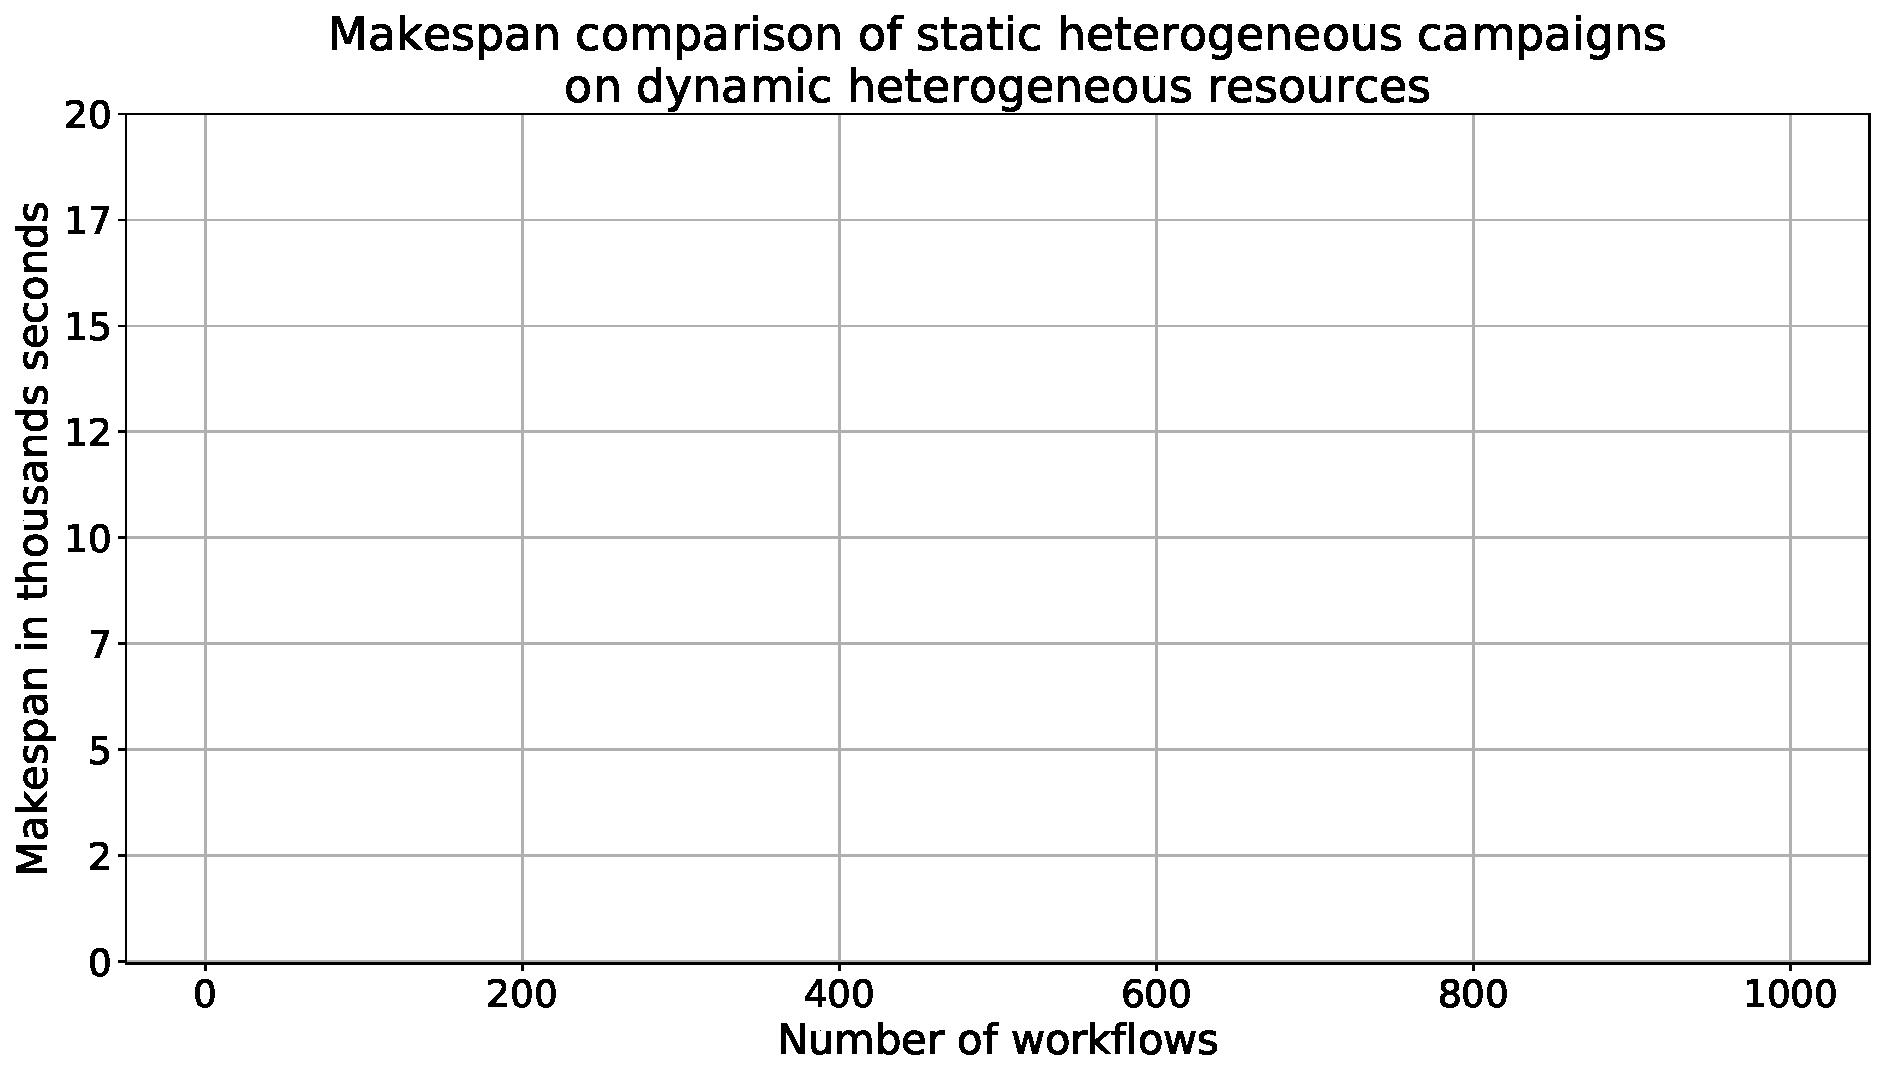
\includegraphics[width=.95\textwidth]{figures/campaign/StHeteroCampaigns_4DyHeteroResources.pdf}
        \caption{}
        \label{fig:StHeteroCampaigns_4DyHeteroResources}
    \end{subfigure}%
    ~ 
    \begin{subfigure}[b]{0.45\textwidth}
        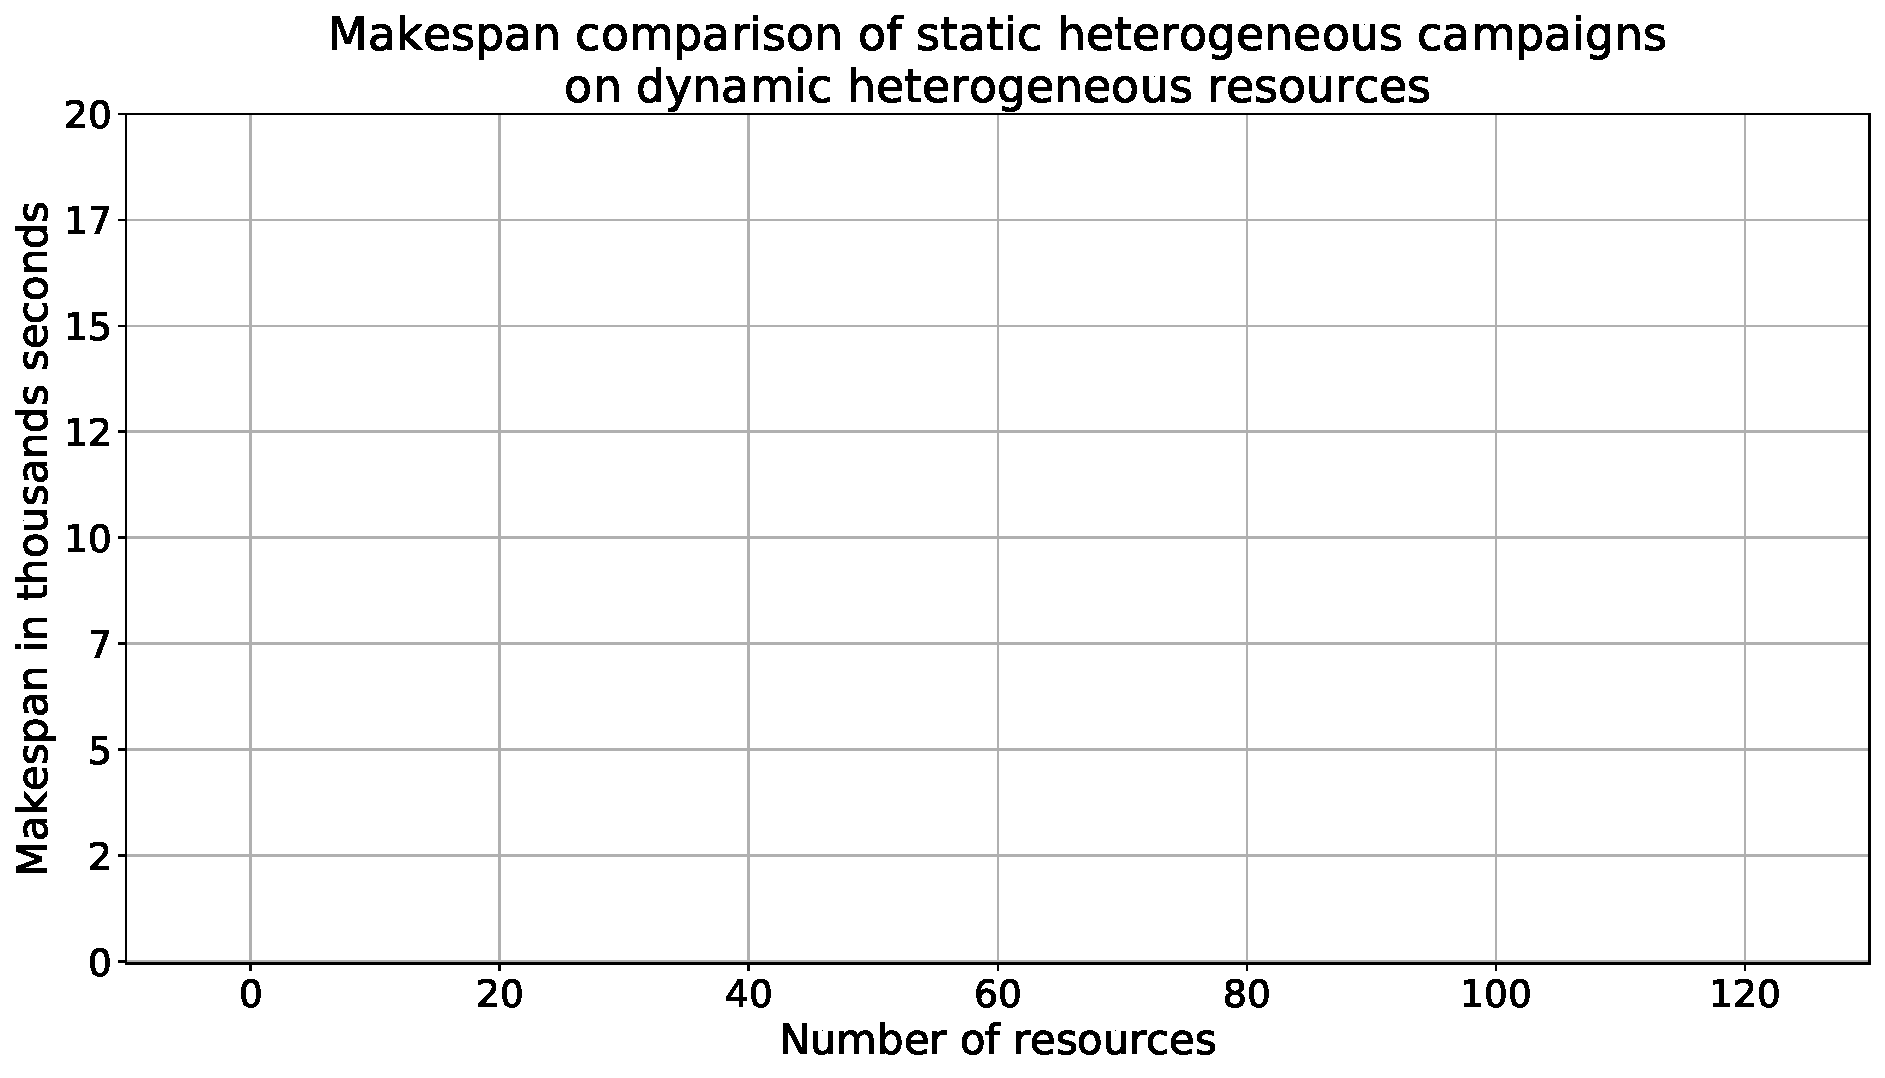
\includegraphics[width=\linewidth]{figures/campaign/DyHeteroResources_StHeteroCampaigns.pdf}
        \caption{}
        \label{fig:DyHeteroResources_StHeteroCampaigns}
    \end{subfigure}
    \caption{~\ref{fig:StHeteroCampaigns_4DyHeteroResources} Makespan of increasing number of homogeneous workflows on homogeneous resources;
    ~\ref{fig:DyHeteroResources_StHeteroCampaigns} Makespan of homogeneous campaign on different number of homogeneous resources.}
    \label{fig:no_replan_hetero_analysis}
\end{figure*}


\subsection{Experiment 3: Workflow Execution Time Accuracy}

Explore how HEFT and GA behave for different resource initial availability if there is time
\begin{figure*}[ht!]
    \centering
    \begin{subfigure}[b]{0.45\textwidth}
        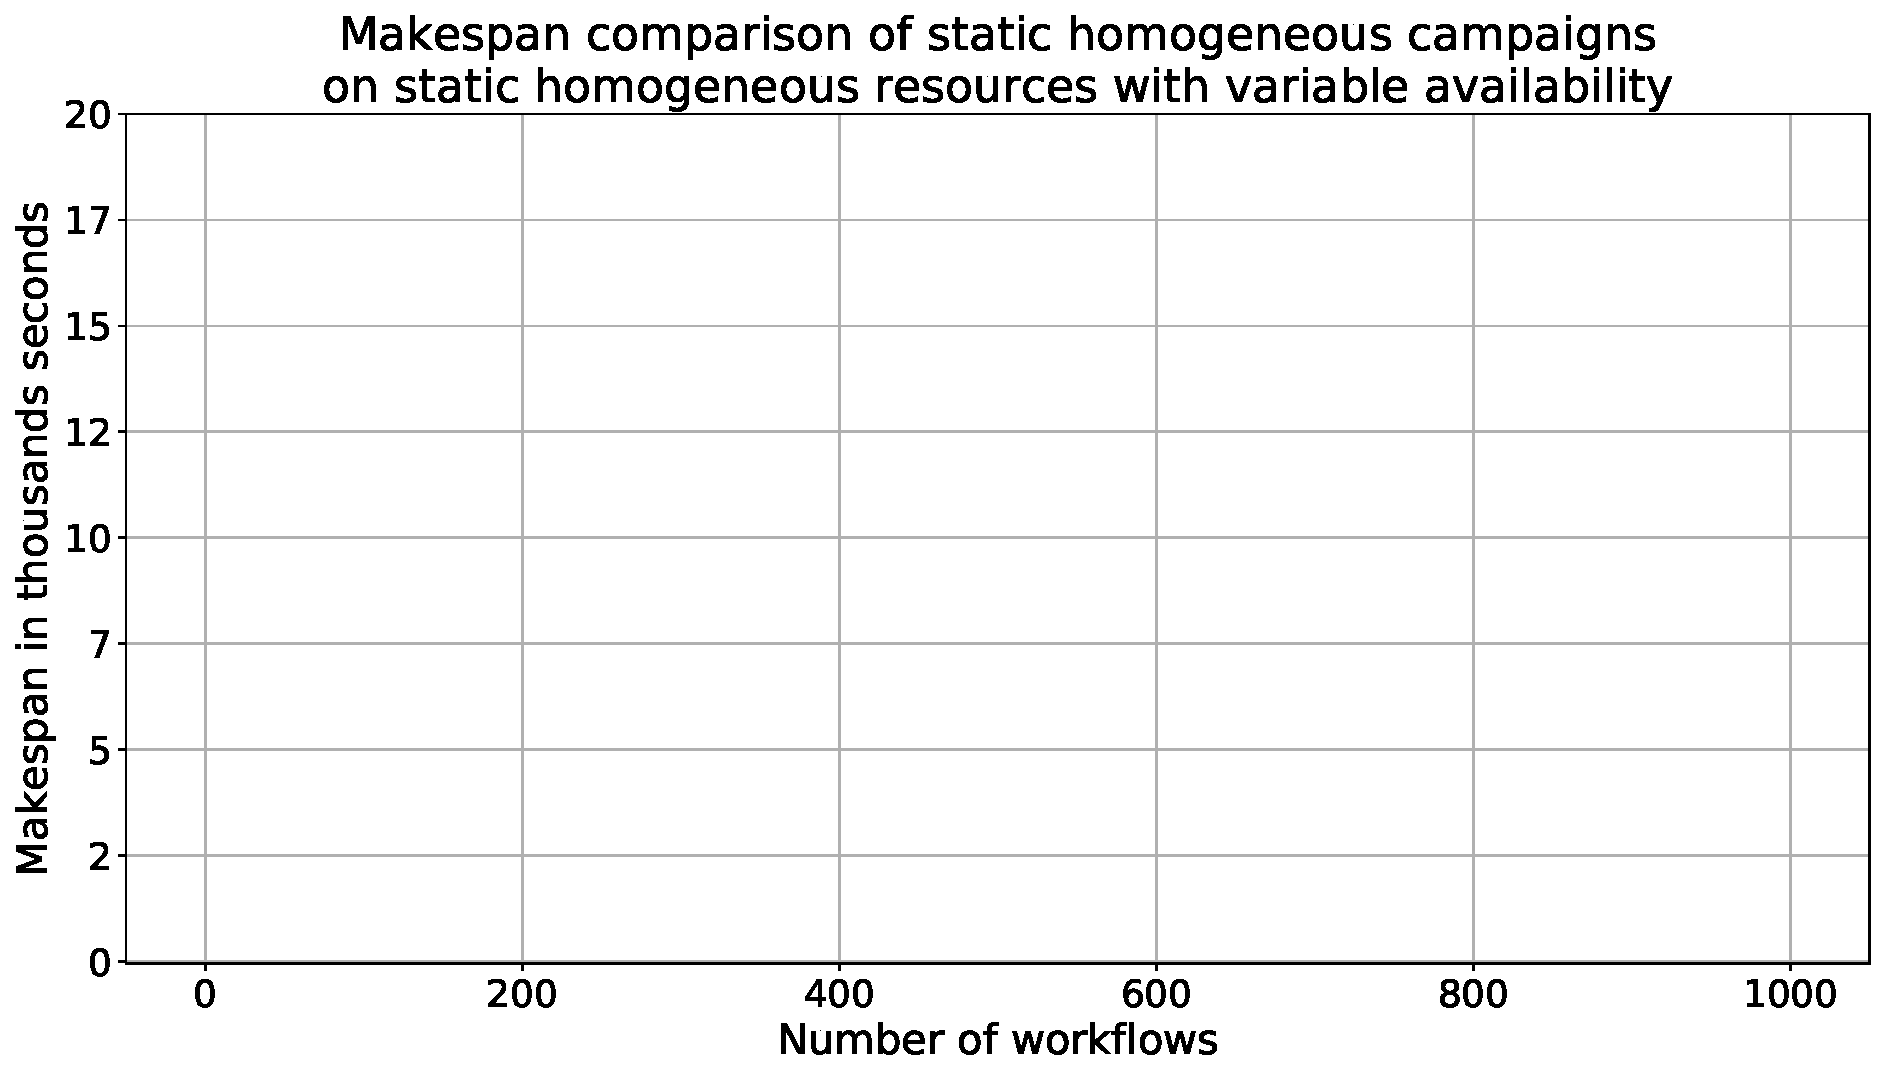
\includegraphics[width=.95\textwidth]{figures/campaign/StHomoCampaigns_4VarHomoResources.pdf}
        \caption{}
        \label{fig:StHomoCampaigns_4VarHomoResources}
    \end{subfigure}%
    ~ 
    \begin{subfigure}[b]{0.45\textwidth}
        \includegraphics[width=\linewidth]{figures/campaign/VarHomoResources_StHomoCampaigns.pdf}
        \caption{}
        \label{fig:VarHomoResources_StHomoCampaigns}
    \end{subfigure}
    \caption{~\ref{fig:StHomoCampaigns_4VarHomoResources} Makespan of increasing number of homogeneous workflows on homogeneous resources;
    ~\ref{fig:VarHomoResources_StHomoCampaigns} Makespan of homogeneous campaign on different number of homogeneous resources.}
    \label{fig:resource_avail}
\end{figure*}

%\subsubsection{Time to calculate a plan}
%
%Based on experiments HEFT and L2FF will have the smallest overhead for calculating the makespan.
%This is due to their deterministic behavior.
%GA on the other hand is a non-deterministic algorithm and its runtime depends on its convergence rate.

\section{Conceptual Framework for Selecting Planning Algorithms}
\label{sec:cf_algo_sel}
Based on our analysis, we conclude that selecting algorithm 1 over algorithm 2 provides the better makespan in most cases. 
But due to the time scales at which the execution of a campaign runs, the computation complexity of the algorithm, as long as, it remains in the order of minutes is not significant.
In addition, selecting an algorithm that can encode resource availability is beneficial, since resources can become unavailable either due to performance dynamism, or due to unforeseen events

% ---------------------------------------------------------
% CHAPTER 7
% ---------------------------------------------------------
\chapter{Conclusions}
\label{ch:conclusions}
\label{ch:conclusions}

\bibliography{general,intro,data_analytics_hpc,designs,campaigns}
\bibliographystyle{unsrt}
\end{document}